\documentclass[a4paper,twoside,spanish,12pt]{report}
\usepackage{pslatex} %utilizar fuentes postscript standard
\usepackage[T1]{fontenc} %codificacion de tipo
\usepackage[spanish]{babel}
\usepackage[latin1]{inputenc} %entrada usando ISO-Latin1
\usepackage{makeidx} %para los indices
\usepackage{amssymb}
\usepackage{amsmath}
\usepackage{euler}
\usepackage{a4wide}
%\oddsidemargin 2.5cm
\usepackage{subfigure}
\usepackage{graphicx}
  \graphicspath{{figures/}}
\usepackage{array}
\providecommand{\tabularnewline}{\\}


\usepackage[boxed,section]{algorithm}
\usepackage{algpseudocode}
\floatname{algorithm}{Algoritmo}
\renewcommand{\listalgorithmname}{Lista de algoritmos}
\usepackage{makeidx}
%\usepackage{hyperref}
%\hypersetup{colorlinks,%
%            pdftex,%
%            linkcolor=black,%
%            citecolor=black,%
%            filecolor=black,%
%            urlcolor=black,%
%						pdfpagemode={None}		}
\frenchspacing
\usepackage[amsmath,framed,thref,hyperref]{ntheorem}

\theoremstyle{break}
\theoremheaderfont{\normalfont\bfseries}
\theorembodyfont{\slshape}
\theoremseparator{:}
\newtheorem{teorema}{Teorema}[section]
\newtheorem{proposicion}{Proposici�}[section]
\newtheorem{lema}{Lema}[section]
\newtheorem{observacion}{Observaci�}[section]
\newtheorem{corolario}[teorema]{Corolario}
\theoremseparator{.}
%\theoremprework{\bigskip\hrule}
%\theorempostwork{\hrule\bigskip}
\newtheorem{definicion}{Definición}[section]

\theoremstyle{change}
\theorembodyfont{\upshape}
\theoremseparator{}
\newtheorem{ejemplo}{Ejemplo}

\theoremstyle{nonumberplain}
\theoremseparator{}
\theoremprework{\relax}
\theorempostwork{\relax}
\newtheorem{demostracion}{Demostración}

 \newenvironment{lyxcode}
   {\begin{list}{}{
     \setlength{\rightmargin}{\leftmargin}
     \setlength{\listparindent}{0pt}
     \raggedright
     \setlength{\itemsep}{0pt}
     \setlength{\parsep}{0pt}
     \normalfont\ttfamily}%
    \item[]}
   {\end{list}}

\usepackage{type1cm}

\makeindex

\pagestyle{headings}

%\renewcommand{\thefootnote}{\roman{footnote}}

\author{David García Quintas}
\title{La librería NumTh}
\date{\today}

\begin{document}

\renewcommand{\tablename}{Tabla}
\maketitle

%\newpage
%
%\vbox to 0.4\textheight{}
%\begin{flushright}
%  \begin{minipage}[t]{13cm}
%    \begin{flushright}
%      \begin{quote}
%        \emph{
%        No estudio más que lo que me place;
%        no ocupo mi espiritu sino en las ideas que me interesan.
%        Estas seran utiles o inutiles para mi o para los demas.
%        El tiempo propiciara o no las circunstancias que me permitiran
%        hacer de mis adquisiciones un empleo provechoso.
%        En todo caso, habre tenido la inestimable ventaja de no contrariarme
%        y de haber obedecido a mi pensamiento y mi carácter.
%        }
%        \begin{flushright}
%          \textbf{\textemdash S. R. N. Chamfort}
%        \end{flushright}
%      \end{quote}
%    \end{flushright}
%  \end{minipage}
%\end{flushright}
%\vfill
%



\newpage

\vbox to 0.4\textheight{}
\begin{flushright}
  \begin{minipage}[t]{8cm}
    \begin{flushright}
      \begin{quote}
        \emph{
        God does arithmetic.
        }
        \begin{flushright}
          \textbf{\textemdash Karl Friedrich Gauss}
        \end{flushright}
      \end{quote}
    \end{flushright}
  \end{minipage}
\end{flushright}
\vfill

\newpage


\tableofcontents
\listoffigures
\listofalgorithms

%%%%%%%%%%%%%%%%%%%%%%%%%%%%%%%%%%%%%%%%%%%%%%%%%%%%%
%d\chapter*{Pr�logo}

\section*{Peque�o apunte sem�ntico}
A lo largo de esta documentaci�n, se ha evitado utilizar el
\emph{relativamente} incorrecto, aunque desafortunadamente ampliamente extendido,
t�rmino �librer�a� para designar el t�rmino t�cnico ingl�s
�library�\footnote{la Real Academia de la Lengua considera ambos
t�rminos sin�nimos. Sin embargo solamente para las acepciones cl�sicas
del t�rmino �librer�a� como local en el cual se tienen libros}.
La definici�n de �library� en este contexto, seg�n el diccionario 
Webster's Revised Unabridged Dictionary (1913): 
\begin{quote}
Library: (...)
   1. A considerable collection of books kept for use, and not
      as merchandise; as, a private library; a public library.
\end{quote}
Es decir, lo que corresponder�a a la definici�n del t�rmino castellano 
�biblioteca�: lugar en el cual se almacena informaci�n lista para su
uso, a \textit{grosso modo} en nuestro caso, funciones; de forma
opuesta a un lugar donde se venden libros. El uso del t�rmino �librer�a�
tendr�a su correspondencia en �bookshop�, como lugar de \emph{venta} de
libros.

Est� claro que esta distinci�n es relativamente trivial por purista en
el uso del lenguaje. Sin embargo, no existe raz�n para no tratar de
tratar de minimizar la impureza en cualquier forma de comunicaci�n. A�n 
con m�s raz�n cuando se trata de llevar a cabo con rigor. No se podr�a
esperar menos de un trabajo que pretende ir de la mano de la estricta
disciplina Matem�tica.  


\section*{Anglicismos}
Es com�n en campos t�cnicos --dominados hoy d�a por la bibliograf�a en 
ingl�s-- el encontrarse con la disyuntiva de utilizar el t�rmino ingl�s,
m�s universal, u optar por una adaptaci�n (ya que en ocasiones siquiera
es posible hablar de �traducci�n�) al castellano. No son pocas las ocasiones
en las que esta segunda opci�n es aplicada, incluso a la fuerza, con resultados
horripilantes. Las razones podr�an argumentarse como de car�cter rom�ntico
hacia el lenguaje propio, por homogeneizar el idioma utilizado como base del
texto, etc. Y no habr�a nada de malo en ninguno de estos casos. Sin embargo
s� lo hay en cuanto la comunicaci�n de las ideas se ve perjudicada por t�rminolog�a
adaptada de forma, podr�a decirse, �creativa�. Ejemplos que ponen los pelos
de punta son el cl�sico �arreglo� para denominar a un ingl�s �array�. Del
mismo modo podr�a optarse por traducir �current� como �corriente� (el�ctica), en vez
de �actual� en contextos como �the current value is...�. En alg�n momento
a alguien se le olvid� que traducir un lenguaje natural implica trabajar con 
un contexto. Cuando el ritmo de cambio de la terminolog�a es mayor que la capacidad
de absorci�n de neologismos en otra lengua dada, se vuelve imprescindible
una unificaci�n de los mismos, si no se quiere caer en un \textit{maremagnum} de
conatos de adaptaciones terminol�gicas con calzador. Hasta que tal cosa ocurra,
es la opini�n del autor que es mejor no introducir a�n m�s ruido en la se�al
ci��ndose al t�rmino m�s extendido, y por tanto m�s claro.

Es por esto que, aun tratando de mantenerlos a un m�nimo, se ha optado por
recurrir al t�rmino en ingl�s cuando un equivalente en castellano universalmente
aceptado no exista.

% CAPITULO DE INTRODUCCI�N

\chapter{Introducci�n}

\begin{flushright}
  \begin{minipage}[t]{13cm}
    \begin{flushright}
      \begin{quote}
        \emph{
    
        BLBLALBLALA


        }
        \begin{flushright}
          \textbf{\textemdash xxxxxxxxxxxxxxxxxxxxx}
        \end{flushright}
      \end{quote}
    \end{flushright}
  \end{minipage}
\end{flushright}

\bigskip

\begin{center}{\line(1,0){325}}\end{center}

%--------------------------------------------------------%
  
\section{Motivaci�n}
  \subsection{�Para qu�?}
   Si el lector no est� familiarizado con el campo de aplicaci�n de
   este tipo de librer�as/herramientas, se�alar su principal campo de
   aplicaci�n, sin detrimento de cualquier otro m�s imaginativo:
   \paragraph{Criptograf�a de clave p�blica.} La propia naturaleza de esta
       familia de m�todos criptogr�ficos necesita manejar n�meros con
       una cantidad elevada de cifras (del orden de cientos o miles de
       cifras). Se da una visi�n m�s en profundidad de este campo en
       la secci�n
       \ref{clavePublica}.

  

\section{Objetivos}
En este proyecto se ha buscado desarrollar una librer�a para el
trabajo en Teor�a de N�meros con la criptograf�a en mente. 
Se ha tratado de dotarla de algunas caracter�sticas distintivas,
as� como las herramientas habituales de estos paquetes. 

Las funcionalidades contempladas han sido:
\begin{itemize}
  \item N�meros enteros, $\mathbb{Z}$
  \begin{itemize}
    \item Enteros de longitud arbitraria.
    \item Aritm�tica general.
    \item Generaci�n de n�meros aleatorios.
    \item Orientadas hacia la Teor�a de N�meros.
    \begin{itemize}
      \item S�mbolos para Residuos Cuadr�ticos
      (Legendre-Jacobi-Kronecker).
      \item Rutinas para el c�lculo del M�ximo Com�n Divisor (GCD).
      \item Rutinas para el c�lculo del M�nimo Com�n M�ltiplo (LCM).
      \item Pruebas de primalidad.
      \item Generaci�n de primos.
      \item Algoritmos de factorizaci�n.
      \item Algoritmos de potenciaci�n.
      \item Teorema Chino de los Restos (CRT).
    \end{itemize}
    \item Aritm�tica modular, $\mathbb{Z}_n$
    \begin{itemize}
      \item Potenciaci�n modular.
      \item M�todos especiales de reducci�n. 
      \item C�lculo de inversas.
      \item Cuerpos Finitos $\mathbb{F}_p$.
    \end{itemize}
  \end{itemize}
  
  \item Conjunto $\mathbb{R}$
  \begin{itemize}
      \item Operaciones aritm�ticas habituales sobre $\mathbb{R}$.
      \item Precisi�n (decimal) arbitraria.
      \item T�cnicas para un redondeo correcto.
      \item Soporte de notaci�n cient�fica.
      \item Algoritmos de potenciaci�n.
  \end{itemize}

  \item Mecanismo de excepciones para el tratamiento de errores.

  \item Arquitectura de "plug-ins" que posibilita que el usuario d� su
    propia implementaci�n de las funciones para ser �sta la utilizada en
    todos los dem�s algoritmos de forma transparente y sin
    recompilaci�n.

  \item Mecanismos de perfilado integrados en la propia librer�a.

\end{itemize}


Seg�n \cite{riesel}\footnote{p�g. 332}, los objetivos principales a la hora de
construir un paquete para c�lculo de precisi�n arbitraria son los
siguientes:
\begin{itemize}
  \item De f�cil uso.
  \item Realizaci�n de los c�lculos con un desempe�o �ptimo.
  \item Introducci�n y obtenci�n de valores sencilla.
  \item Requisitos de almacenamiento m�nimos.
  \item Adaptable a diferentes entornos y arquitecturas.
\end{itemize}
Ahora bien, como suele ser habitual, no es posible conjugar
simult�neamente todos estos aspectos. Pero a�n as�, merece la pena
tratar de acercarse. Las medidas tomadas en el presente proyecto
para conseguirlo han sido, en t�rminos generales, las siguientes:
\paragraph{Orientaci�n a objetos y sobrecarga de operadores.}
  Mediante la utilizaci�n de un lenguaje que ofrezca estos mecanismos
  se consigue por una parte una mejor organizaci�n del c�digo con una
  mayor ``coherencia jer�rquica'' entre los diferentes elementos. La
  sobrecarga de operadores es fundamental a la hora de prestar
  servicios de forma pr�cticamente transparente al usuario, quien por
  ejemplo podr� seguir sumando del mismo modo tipos b�sicos del
  sistema y los nuevos tipos num�ricos ofrecidos.
\paragraph{Buenos algoritmos.}
  Aunque pudiera parecer de perogrullo, la elecci�n de los
  algoritmos (dejando ya de lado su implementaci�n) para cada tarea
  no es una tarea trivial: la variedad de los mismos y sus
  diferentes ventajas y defectos hacen que se requiera un
  concienzudo estudio previo a la elecci�n.
\paragraph{Portabilidad.}
  Es deseable que el c�digo no se quede relegado a una sola plataforma
  o sistema. Y m�s a�n si estamos hablando de una librer�a. Es por
  esto que se ha tenido cuidado en escribir un c�digo portable de
  forma directa (sin m�s que recompilar el c�digo C++), controlando
  aquellas partes dependientes del sistema reduci�ndolas a un m�nimo y
  siempre justificando su car�cter no portable. A este respecto, ver
  la secci�n \ref{elProcesadorVirtual}.

  \subsection{Caracter�sticas a destacar}
    Anteriormente se cit� que una de las razones del desarrollo de
    esta librer�a es suplir, en la medida de lo posible, algunos
    aspectos de otros paquetes con la misma orientaci�n. As�, se puede
    considerar que el presente Proyecto brinda algunas caracter�sticas
    a destacar por no haberse encontrado, una u otra, en las dem�s
    librer�as afines que se han examinado (las citadas en
    \ref{libreriasSimilares}).
    \begin{itemize}
      \item El uso de la orientaci�n a objetos es mucho mayor y m�s
        adecuado. Esto es debido a que en los casos en los que la
        librer�a examinada utilizaba C++, en realidad era una
        adaptaci�n desde una implementaci�n previa en C, con lo cual
        en realidad no deja de ser una implementaci�n en C ``con
        clases''. Ejemplo de esto es que en la librer�a NTL, la
        representaci�n interna de los n�meros (algo que a todas luces
        ha de ser invisible para el usuario) tiene categor�a
        \texttt{public}.
      \item La librer�a est� preparada para soportar hilos\footnote{El
        t�rmino ingl�s y m�s extendido para esto es ``thread safe''}.
        Esto es muy importante desde el punto de vista de la posible
        paralelizaci�n de los algoritmos. Por lo general, otras
        librer�as no lo soportan debido al uso relativamente frecuente
        de variables globales con las consecuencias que ello tiene en
        este aspecto: problemas de interbloqueo, sincronizaci�n, etc.
      \item Soporte de perfilado integrado en la librer�a. La causa de
        que esto sea algo �nico de esta librer�a es bastante claro: las
        dem�s conf�an en herramientas externas y por otra parte suelen
        buscar el rendimiento m�ximo. La presente librer�a tambi�n
        busca el m�ximo rendimiento, claro est�, pero se ha
        considerado interesante la inclusi�n de esta caracter�stica,
        siendo adem�s opcional su activaci�n. V�ase \ref{perfilado} para m�s
        detalles.
      \item Soporte de excepciones para el manejo de errores. Las
        librer�as analizadas recurr�an a m�todos ``cl�sicos'' como los
        expuestos en \ref{controlDeErrores}. Por contra, y como se
        expone en dicha secci�n, esta librer�a hace uso del mecanismo
        de excepciones que C++ brinda, con las ventajas all�
        expuestas.
      \item Soporte de ``funciones enchufables''. Esta es una de las
        caracter�sticas m�s destacadas de la librer�a. A grandes
        rasgos, permite que el usuario, sin necesidad de tocar para
        nada el c�digo de la librer�a, proporcione su propia
        implementaci�n de los algoritmos para las funciones num�ricas
        soportadas, y que esta implementaci�n sea utilizada incluso
        internamente por la librer�a a partir del punto en el que el
        usuario la hace entrar en vigor. Para una descripci�n m�s en
        detalle, v�ase \ref{funcionesBasico}.
    \end{itemize}

\section{El sistema de desarrollo}\label{sistemaDeDesarrollo}
  En la elaboraci�n de este proyecto se han utilizado diversas
  herramientas y sistemas.sistemaDeDesarrollo} Aqu� se da un resumen de lo utilizado en
  parte a modo de curiosidad y en parte como configuraciones en las
  que se sabe que la librer�a funciona correctamente.
  \subsection{Sistemas hardware}
  \begin{description}
    \item[Plataforma compatible Intel.] 
      Sistema con microprocesador AMD Athlon K7 funcionando a una
      frecuencia de 900 MHz. Esta ha sido la plataforma hardware
      principal en el desarrollo.
  \end{description}

  \subsection{Sistemas software}
  En este grupo se distinguen distintos ``niveles''. Se citan los
  distintos elementos con una cierta jerarqu�a.
  \begin{description}
    \item[Sistema operativo Linux.]
      En sus versiones 2.4.x y 2.6.x. Ha sido el sistema operativo
      principal en el desarrollo. Los distintos programas y versiones
      de librer�as fundamentales del sistema han sido:
      \begin{description}
        \item[Librer�as del sistema.] 
          Implementaci�n GNU de la librer�a de C, versi�n 2.3.2.
        \item[Librer�as adicionales.]
          Librer�a Qt versi�n 3.3.0 para el desarrollo del interfaz gr�fico de la
          aplicaci�n de demostraci�n expuesta en \ref{laCalculadora}.
        \item[Compilador.]
          Compilador GNU Compiler Collection (GCC).
          Versi�n principal usada en el desarrollo 3.3.3. Realizadas
          pruebas en diferentes versiones hasta la 3.2 inclusive.
        \item[Documentaci�n.]
          Procesador de documentos \LaTeXe{} y \TeX{} versi�n 3.14159
          \footnote{Un inciso curioso: las versiones de \TeX{} se numeran de
          forma convergente al valor de $\pi$} para la presente
          documentaci�n.
          Procesador Doxygen versi�n 1.3.6 para el procesador de la
          documentaci�n del c�digo.
        \item[Edici�n.]
          Editor VIM versi�n 6.2 para la escritura del c�digo y la documentaci�n. 
          (Con la excepci�n del dise�o del interfaz de la aplicaci�n
          de demostraci�n expuesta en \ref{laCalculadora} donde se
          utiliz� Qt Designer versi�n 3.3.0).
          Editor de diagramas Dia versi�n 0.92.2 para la creaci�n de los
          diagramas presentes en la documentaci�n.
      \end{description}
      Parece adecuado destacar que todo el software anteriormente
      rese�ado es \emph{software libre}. Y es m�s, ha sido
      precisamente gracias a que mucho del mejor software cient�fico
      disponible tambi�n es software libre que a lo largo del
      desarrollo de esta librer�a se ha podido examinar y aprender
      much�simo de la forma en la que, personas con a�os de experiencia
      en la creaci�n de este tipo de software, resuelven e implementan
      los problemas que se van presentando. Mi deuda para con todos
      ellos, creadores de software libre, es grande.
      
    \item[Sistema operativo Windows.]
      En sus versiones 2000 y XP. Se ha restringido su uso al de
      simplemente banco de pruebas y como muestra de la portabilidad
      de la librer�a entre sistemas en una misma plataforma hardware
      ---Intel, en este caso.
      Los distintos programas y versiones
      de librer�as fundamentales del sistema han sido:
      \begin{description}
        \item[Librer�as adicionales.]
          Librer�a Qt versi�n 3.2.1 para el desarrollo del interfaz gr�fico de la
          aplicaci�n de demostraci�n expuesta en \ref{laCalculadora}.
        \item[Compilador.]
          Adaptaci�n del compilador GNU Compiler Collection (GCC) para
          entornos Windows MinGW.
          Versi�n principal usada en el desarrollo 3.3.1. 
      \end{description}
    \end{description}
      

% CAPITULO SOBRE LA IMPLEMENTACION DE XXX

\chapter{ XXX }\label{cap:XXX}

\begin{flushright}
  \begin{minipage}[t]{13cm}
    \begin{flushright}
      \begin{quote}
        \emph{

          xxxxxxxxxxxxxxxxxxxx

        }
        \begin{flushright}
          \textbf{\textemdash xxxxxxxxxxxxx}
        \end{flushright}
      \end{quote}
    \end{flushright}
  \end{minipage}
\end{flushright}

\bigskip

\begin{flushright}
  \begin{minipage}[t]{13cm}
    \begin{flushright}
      \begin{quote}
        \emph{

        xxxxxxxxxxxxxxxxxxxxxxxx

        }
        \begin{flushright}
          \textbf{\textemdash xxxxxxxxxxxxx}
        \end{flushright}
      \end{quote}
    \end{flushright}
  \end{minipage}
\end{flushright}

\bigskip

\begin{center}{\line(1,0){325}}\end{center}

%--------------------------------------------------------%

\section{Introducci�n}


\chapter{Paralelismo en la biblioteca}

\begin{flushright}
  \begin{minipage}[t]{13cm}
    \begin{flushright}
      \begin{quote}
        \emph{
          Right now I'm having amnesia and d�j� vu at the same time.
        }
        \begin{flushright}
          \textbf{\textemdash Stephen Wright (en paralelo).}
        \end{flushright}
      \end{quote}
    \end{flushright}
  \end{minipage}
\end{flushright}

\bigskip

\begin{center}{\line(1,0){325}}\end{center}

%--------------------------------------------------------%

\section{Introducci�n}

  Se ha hecho �nfasis en la paralelizaci�n de los m�todos b�sicos sobre los 
  que la mayor�a de las rutinas de m�s alto nivel se apoyan. Por varios motivos:
  \begin{description}
    \item[Por su propia naturaleza.] Como m�todos \emph{b�sicos}, son utilizados con 
    mucha mayor frecuencia, y por un abanico mayor de clientes. Cualquier optimizaci�n
    --en este caso la paralelizaci�n-- tendr� un efecto beneficioso directamente proporcional 
    dichos factores.
    \item[Facilidad.] La complejidad de los m�todos suele ser mayor en m�todos de m�s alto nivel.
    Por ejemplo, comp�rese la complejidad de los m�todos de factorizaci�n de enteros con la implementaci�n
    b�sica del producto de enteros. Es incluso probable que la adaptaci�n paralela de los actuales 
    m�todos secuenciales no sea posible sin una reescritura completa del m�todo. N�tese sin embargo como,
    en base al punto anterior, incluso los complejos m�todos no paralelizables s� se benefician de la paralelizaci�n
    de los b�sicos: siguiendo con el ejemplo de la factorizaci�n y el producto de enteros, el primer m�todo s� se valdr�
    del segundo y ser� \emph{parcialmente} paralelo de forma indirecta.
    \item[Modularidad.] Un m�todo b�sico es susceptible de ser reutilizado en alg�n otro lugar, haciendo gala de su
    modularidad. Consigo arrastrar� su condici�n de paralelo, haciendo extensiva esta caracter�stica incluso all� 
    donde no se ha hecho un esfuerzo expl�cito en este sentido. 
  \end{description}




  \subsubsection{Especificaci�n del paralelismo}
    Desgraciadamente, no existe una sintaxis universalmente aceptada para la especificaci�n
    de algoritmos paralelos. No ser� en esta memoria donde se contribuya a empeorar a�n m�s esta
    situaci�n, sino que nos ce�iremos a la sintaxis del la tecnolog�a utilizada para la obtenci�n
    de paralelismo en nuestros m�todos, OpenMP. Esto conlleva que el lector habr� de estar al menos
    parcialmente familiarizado con la sintaxis de este interfaz. Afortunadamente, no se trata de una
    familia de m�todos bastante reducida y de f�cil interpretaci�n. Para una introducci�n de apenas
    veinte p�ginas --pero ya suficiente para la comprensi�n del c�digo aqu� incluido--, v�ase 
    el ap�ndice A de \cite{parpatterns}. En cualquier caso, en la opini�n del autor, la mayor�a de 
    los ejemplos de c�digo son autoexplicativos aun utilizando las directivas de OpenMP.







\section{Potenciaci�n modular}
  \subsection{Dos hilos y $\mathbb{Z}M_n$}
  \cite{modexpmont}
  \subsection{Mi m�todo}

\section{Vectores}
  \subsection{Producto escalar}

\section{Matrices}
  \subsection{Producto}
  \subsection{Descomposici�n $LU$}
  \subsection{Inversi�n}
  \subsection{Transposici�n}
  \subsection{Determinante}
    \subsubsection{Algoritmo de Gauss-Bareiss}\label{para:bareiss}
    Descrito en la secci�n \ref{impl:bareiss}. Si se representa el patr�n de accesos derivado 
    de su algoritmo secuencial (algoritmo \ref{alg:bareiss}), no es dif�cil derivar una divisi�n
    en tareas basada en la secuencia de patrones de dise�o 
    (data decomposition/order tasks -> geom. decomposition -> loop paralelism)
    de \cite{parpatterns}. En la figura \ref{fig:accBar} 
    se muestra el patr�n de accesos para el algoritmo.  Los elementos de color verde
    indican accesos de \emph{lectura}, mientras que los de color rojo indican tambi�n \emph{escritura}.

   \begin{figure}[h]
    \centering
    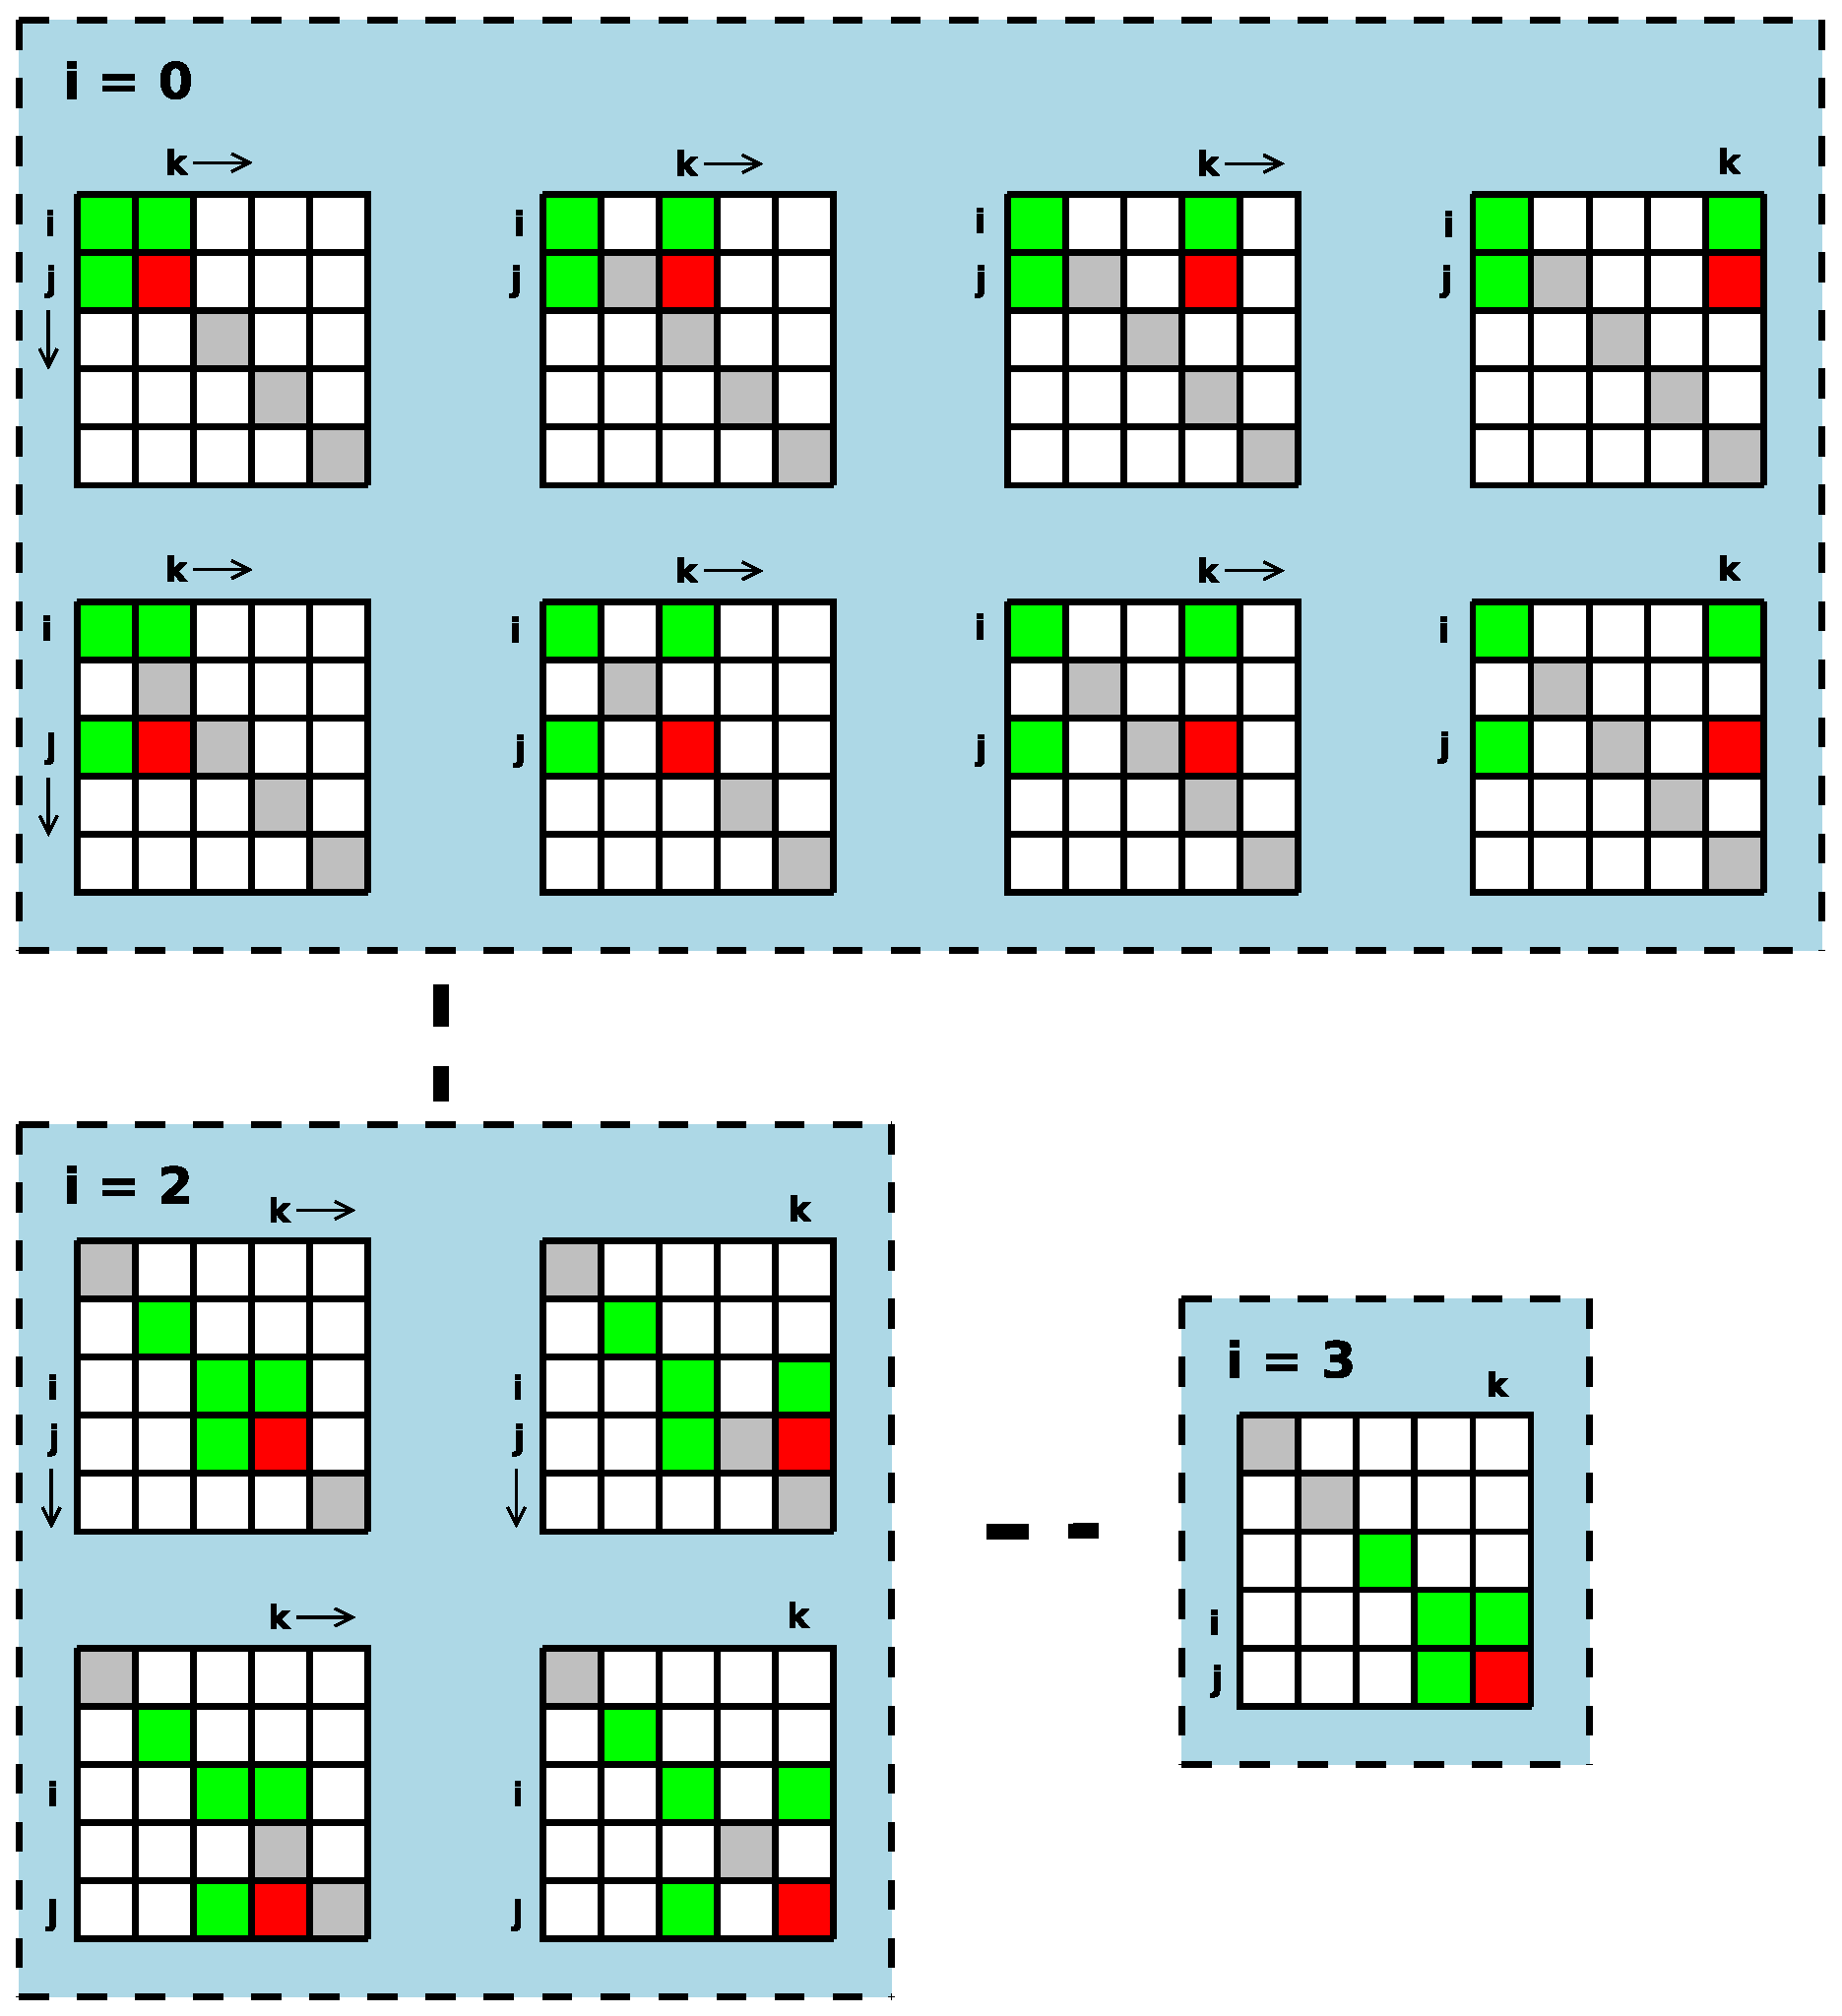
\includegraphics[width=0.95\textwidth,keepaspectratio]{patronAccesosBarreis} 
    \caption{Patr�n accesos Gauss-Bareiss}\label{fig:accBar}
  \end{figure}

  De este patr�n de acceso se deriva una paralelizaci�n organizada por el acceso a los datos y
  con una enumeraci�n lineal. Por tanto el patr�n estructural m�s indicado parece ser una descomposici�n
  geom�trica sobre las filas, siguiendo el recorrido de $k$. A nivel de estructura de soporte, el patr�n de 
  paralelismo de bucle se ajusta perfectamente: %FIXME

      \begin{algorithm}
        \caption{Algoritmo de Gauss-Bareiss}\label{alg:bareiss}
        \begin{algorithmic}[1]
          \Procedure{Gauss-Bareiss}{Matriz $M \in \mathcal{M}_{n \times n}$}
          \State $sign \gets 1$
          \For{$i \in \{0, \ldots, n-2\}$}
            \State $p \gets M_{i,i}$
            \If{$p = 0$}
              \If{$ \neg \mathrm{pivot(}$i$\mathrm{)} $} 
                \Statex \Comment{Si \textrm{pivot} es falso, no se ha podido pivotar}
                \State \textbf{Return} $0$ \Comment{Matriz singular}
              \EndIf
              \State $sign \gets -sign$ \Comment{Se ha permutado una fila}
              \State $p \gets M_{i,i}$ \Comment{$M_{i,i} \neq 0$}
            \EndIf
            \State \texttt{\#pragma omp parallel}
            \For{$j \in \{i+1,\ldots,n-1\}$}
              \State \texttt{\#pragma omp for}
              \For{$k \in \{i+1,\ldots,n-1\}$}
                \State $M_{j,k} \gets M_{j,k} * p - M_{j,i}*M_{i,k}$
                \If{ $i > 0$ }
                  \State $M_{j,k} \gets M_{j,k} / M_{i-1,i-1}$ \Comment{Esta divisi�n \emph{siempre} es exacta}
                \EndIf
              \EndFor %for k
            \EndFor %for j
          \EndFor %for i

          \State \textbf{Return } $sign * M_{n-1,n-1}$
          \EndProcedure
        \end{algorithmic}
      \end{algorithm}



  \subsection{Operaciones de car�cter vectorial}
    % sumas, restas, prod por escalares

\section{C�lculo de \textit{reducciones}}


\section{Polinomios}
  \subsection{Producto}
  \subsection{Operaciones de car�cter vectorial}
    % sumas, restas, prod por escalares
  \subsection{Evaluaci�n}\label{parallel:evalPoly}
    \cite{dorn}



%% CAPITULO SOBRE LOS FUNDAMENTOS MATEM�TICOS

\chapter{Fundamentos matem�ticos}

\begin{flushright}
  \begin{minipage}[t]{13cm}
    \begin{flushright}
      \begin{quote}
        \emph{
        \ldots both Gauss and lesser mathematicians may be justified
        in rejoicing that there is one science [number theory] at any
        rate, and that their own, whose very remoteness from ordinary
        human activities should keep it gentle and clean.
        }
        \begin{flushright}
          \textbf{\textemdash G. H. Hardy, ``A Mathematician's Apology''}
        \end{flushright}
      \end{quote}
    \end{flushright}
  \end{minipage}
\end{flushright}

\begin{flushright}
  \begin{minipage}[t]{13cm}
    \begin{flushright}
      \begin{quote}
        \emph{
        It seems strange that on one hand the most practical of disciplines, 
        namely, physics has connections with the most arcane of disciplines,
        namely, number theory. However, surprising connections have appeared
        betwen number theory and physics...The work of Ramanujan in particular
        has had surprising connections with string theory, conformal field
        theory and statistical physics.
        }
        \begin{flushright}
          \textbf{\textemdash R. Padma y H. Gopalkrishna Gadiyar, 
                             ``Renormalisation and the density of
                             prime pairs''}
        \end{flushright}
      \end{quote}
    \end{flushright}
  \end{minipage}
\end{flushright}




\begin{center}{\line(1,0){325}}\end{center}

%--------------------------------------------------------%

\section{Introducci�n}
En este cap�tulo se presentan conceptos y resultados dentro de la
Matem�tica, normalmente de la Teor�a de N�meros, que sientan los
pilares b�sicos sobre los que descansan muchos de los resultados que
ser presentan tanto en la presente librer�a como en la criptograf�a en
general.

\section{Teor�a de la complejidad}\label{teoriaDeLaComplejidad}
La teor�a de la complejidad sirve para proporcionar una referencia en
el marco de la eficiencia de los algoritmos. Su importancia a la hora
de servir de herramienta en el desarrollo de m�todos criptogr�ficos es
fundamental, ya que se ha de ser capaz de estimar la ``dureza'' de un
m�todo para asegurarse, por ejemplo, de que �ste no sea susceptible de
ser atacado por fuerza bruta (esto es, probando todo el n�mero de
claves posibles).

  \subsection{Clases de complejidad}\label{clasesDeComplejidad}
  La complejidad de un algoritmo va en relaci�n directa con la
  cantidad de esfuerzo computacional necesario para ejecutarlo, siendo
  este ``esfuerzo'' no necesariamente potencia de procesamiento, sino
  que tambi�n puede ser necesidades de almacenamiento. De nada nos
  servir�a tener un algoritmo rapid�simo si consume grandes cantidades
  de memoria y es requisito implementarlo en, por ejemplo, un
  microprocesador de se�ales como el que puede llevar un reproductor
  de m�sica portatil\footnote{si el lector se percata por el t�tulo, en \cite{barrett},
  donde se expone el m�todo de exponenciaci�n modular utilizado por la
  librer�a, se ten�a el objetivo de implementar el algoritmo RSA en
  uno de estos microprocesadores}.
  A�n as�, salvo que se diga lo contrario, en lo sucesivo se
  considerar� la complejidad \emph{temporal}, esto es, de potencia de
  procesamiento.
   
  \begin{figure}\label{fig:clasesComplejidad}
    \begin{center}
      \subfigure[Conjunto general]{\label{subfig:conjuntoGeneral}
      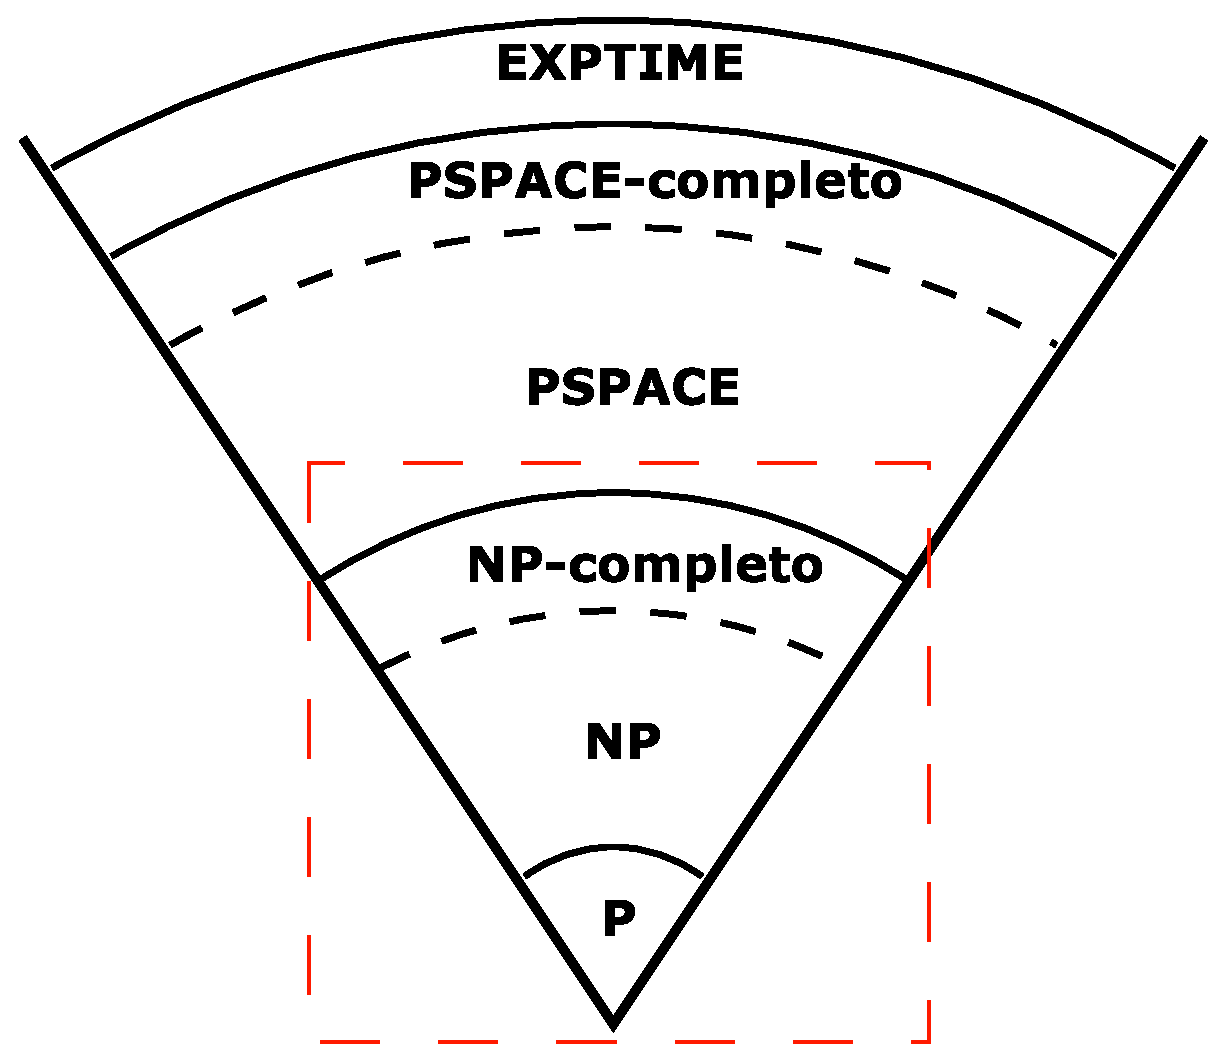
\includegraphics[width=0.45\textwidth,keepaspectratio]
      {clasesComplejidad1}
    }
    \subfigure[Detalle clases
    temporales]{\label{subfig:detalleClasesTemporales}
      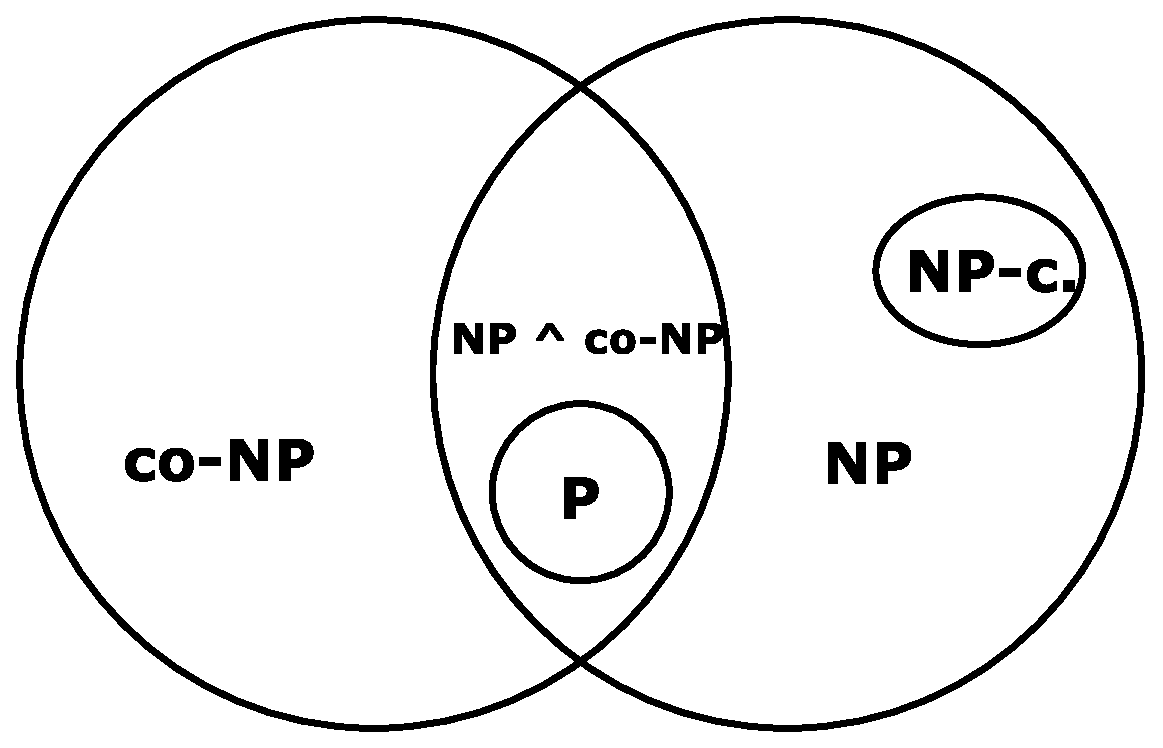
\includegraphics[width=0.45\textwidth,keepaspectratio]
      {clasesComplejidad2}
    }
    \end{center}
    \caption{Clases de complejidad}
  \end{figure}
 
  Se cuenta con distintas \index{clases!de complejidad}{\emph{clases
  de complejidad}} en funci�n de la forma de su cota ``O grande'',
  cuyo argumento $n$ suele ser el tama�o de la entrada del problema.
  En la figura \ref{subfig:conjuntoGeneral} se muestra un esquema de
  la familia de clases de complejidad, con la parte recuadrada en
  l�nea discont�nua ampliada en \ref{subfig:detalleClasesTemporales}.
  
  \begin{itemize}
    \item Un algoritmo cuyo tiempo de ejecuci�n est� en
      $O(1)$ se denomina \emph{constante}.
    \item Un algoritmo cuyo tiempo de ejecuci�n est� en
      $O(n)$ se denomina \emph{lineal}.
    \item Un algoritmo cuyo tiempo de ejecuci�n est� en
      $O(n^2)$ se denomina \emph{cuadr�tico}; si est� en $O(n^3)$
      \emph{c�bico}, etc.
  \end{itemize}
  Hasta aqu�, se estar�a en la clase de complejidad \textbf{P},
  representando la clase de algoritmos de \index{tiempo!polinomial}{\emph{tiempo polinomial}}, 
  que responden a la forma general $O(n^k)$ con $k$ constante.
  Siempre que nos refiramos a que una determinada computaci�n es
  \index{computaci�n!f�cil}{``f�cil''} o \index{computaci�n!eficiente}{``eficiente''} y 
  a que un problema es \index{problema!tratable}{``tratable''}, se entender� 
  que pertenece a esta clase de complejidad. Por otra parte, todo
  algoritmo fuera de esta clase se denominar� respectivamente 
  \index{computaci�n!dif�cil}{``dif�cil''}, \index{computaci�n!ineficiente}{``ineficiente''} e 
  \index{problema!intratable}{``intratable''}.
      
  Los algoritmos acotados por $O(k^{f(n)})$, con $k > 1$ una constante
  y $f(n)$ una funci�n polinomial de $n$, son denominados de 
  \index{tiempo!exponencial}{\emph{tiempo exponencial}}. Un ejemplo
  cl�sico de esta clase son los algoritmos con cota $O(2^n)$. La
  subclase en los que la funci�n $f(n)$ es menos que lineal pero m�s
  que constante (por ejemplo, $f(n) \equiv \log(n)$) son denominados 
  de \index{tiempo!superpolinomial}{\emph{tiempo superpolinomial}}.
  Estos algoritmos de tiempo exponencial conformar�an la clase de
  complejidad \textbf{EXPTIME}. Un algoritmo criptografico de esta
  complejidad es el regocijo de quien lo implementa y la pesadilla de
  quien intente romperlo por fuerza brutal, ya que en la pr�ctica
  resulta inabordable.

  En \cite{schneier}\footnote{p�g. 239, tabla 11.2} se da una tabla
  que resulta muy significativa e ilustra de lo que realmente se est�
  hablando con estas cotas. Se reproduce en la tabla \ref{tablaClases}
  \begin{table}
    \begin{center}\begin{tabular}{|c|c|c|c|} 
      \hline
      Clase & Complejidad & Operaciones para $n=10^6$ & Tiempo a
      $10^6$ op./seg.\tabularnewline
      \hline
      \hline 
      Constante & $O(1)$ & $1$ & $1$ $\mu$seg.\tabularnewline
      \hline 
      Lineal & $O(n)$ & $10^6$ & $1$ seg.\tabularnewline
      \hline 
      Cuadr�tica & $O(n^2)$ & $10^{12}$ & $11.6$ d�as\tabularnewline
      \hline 
      C�bica & $O(n^3)$ & $10^{18}$ & $32000$ a�os\tabularnewline
      \hline 
      Exponencial & $O(2^n)$ & $10^{301030}$ & $10^{301006}$ veces la edad del Universo\tabularnewline
      \hline 
    \end{tabular}\end{center}
    \caption{Ejemplos de tiempos para algunas cotas de complejidad}
    \label{tablaClases}
  \end{table}


  La clase \textbf{NP} es un poco m�s sutil. 
  Est� compuesta por aquellos problemas que ``pueden ser resueltos en
  tiempo polinomial �nicamente en una m�quina de Turing no
  determin�stica'' (\cite{schneier}\footnote{p�g. 240}). Esto
  simplemente quiere decir que un algoritmo en esta clase que intente
  dar respuesta a un problema determinado, intentar� ``adivinar'' la
  respuesta y comprobar� en tiempo polinomial (mediante un algoritmo
  en \textbf{P}) si �sta es correcta.
  Aunque a primera vista esta definici�n puede parecer extra�a, tras
  un momento de reflexi�n puede uno darse cuenta f�cilmente de que
  este esquema es precisamente el que sigue, por ejemplo, el problema
  de factorizaci�n de enteros (secci�n \ref{factoring}): comprobar si
  se ha encontrado un factor no trivial se puede hacer en tiempo
  polinomial (concretamente en $O(n^2)$), mientras que la b�squeda de
  este factor actualmente (primera mitad de 2004) se reduce, con
  m�todos m�s o menos sofisticados, a un proceso ``adivinatorio''.
  Es evidente que la clase \textbf{NP} incluye a la clase \textbf{P}.
  Lo que de verdad s� resulta sorprendente es el desconocimiento de si
  se verifica $\textbf{P} = \textbf{NP}$\footnote{si el lector es
  asiduo, como el autor, a la serie Los Simpsons (y adem�s es
  observador), quiz�s se haya dado cuenta de que en el cap�tulo en el
  que Homer se introduce en un v�rtice y acaba llegando a una especie
  de ``dimensi�n matem�tica'' donde hay f�rmulas flotando tales como
  $e^{i\pi} = -1$, tambi�n se encuentra $\textbf{P} = \textbf{NP}$}
  , aunque parece ser (\cite{schneier}\footnote{p�g. 241}) que los
  expertos opinan que esta igualdad \emph{no} se verifica.

  Existe tambi�n una clase de complejidad \textbf{NP-completo}, a la
  que pertenecen aquellos problemas de \textbf{NP} que se demuestra que son tan 
  complejos como cualquier otro de esta clase. Es interesante hacer
  notar que esto implica que si se demuestra que \emph{cualquier} problema
  perteneciente a \textbf{NP-completo} est� tambi�n en \textbf{P}, se
  demostrar�a que $\textbf{P} = \textbf{NP}$. Este es un tema amplio
  que no se tratar� aqu�, pero del que se puede encontrar informaci�n
  en \cite{brassard}\footnote{Todo su cap�tulo 12}.

  Respecto a la clase \textbf{co-NP} que aparece en la
  figura \ref{subfig:detalleClasesTemporales}, coincide con la
  clase \textbf{NP} salvo por el hecho de que da respuestas
  \emph{negativas}: representa los problemas para los cuales una
  respuesta negativa puede ser comprobada en tiempo polinomial.
  
  Las clases \textbf{PSPACE} y \textbf{PSPACE-completo} responden a
  problemas que pueden ser resueltos con unas necesidades de \emph{espacio}
  polinomiales, aunque no necesariamente en en tiempo polinomial. Lo
  dicho para \textbf{NP-completo} se aplica tambi�n a
  \textbf{PSPACE-completo}.


  \subsection{Problemas fundamentales}\label{problemasFundamentales}
  Bajo esta etiqueta de ``fundamentales'' se encuentran aquellos
  problemas utilizados habitualmente como referencia a la hora de, en
  criptograf�a, contar con una base que de ciertas garant�as de
  intratabilidad. Esta intratabilidad ser� de la que se valgan los
  esquemas de tipo ``puerta trasera'' (v�ase secci�n \ref{funcionesTrapdoor}) y, 
  m�s concretamente, los mecanismos de criptograf�a de clave p�blica
  (v�ase secci�n \ref{clavePublica}).

  Estos problemas, al calificarlos como ``intratables'', se quiere dar
  a entender que \emph{no} pertenecen a la clase de complejidad
  \textbf{P}, tal y como se expuso en \ref{teoriaDeLaComplejidad}.
  Ahora bien, no est� demostrado, en general, que sean intratables
  (\cite{handbook}\footnote{p�g. 87}); es m�s, en el modelo de
  computaci�n basado en la mec�nica cu�ntica\footnote{Esto est� fuera
  del alcance de esta memoria, pero en \cite{feynman} se puede
  encontrar una introducci�n \emph{asequible} a la computaci�n cu�ntica} 
  , es posible el c�lculo en \textbf{P} de logaritmos discretos y la
  factorizaci�n de enteros, mediante el algoritmo debido a Peter Shor.
  Se exponen estos m�todos en \cite{shor}. Y no s�lo esto, sino que en
  \cite{handbook}\footnote{p�g. 130, �ltimo p�rrafo} se expone c�mo,
  mediante t�cnicas de biolog�a molecular utilizando DNA, se puede
  resolver el conocido problema de los caminos Hamiltonianos en un
  tiempo mucho menor que con los tradicionales ordenadores
  electr�nicos.
  
  Hasta podr�a darse el (improbable) caso de que efectivamente $\textbf{P} = \textbf{NP}$.
  Sea como fuere, parece bastante probable que este campo depare a�n
  muchas sorpresas. Que as� sea.
  

  A la hora de establecer relaciones entre estos problemas
  fundamentales, ha de contemplarse lo siguiente
  (\cite{handbook}\footnote{pp. 88,89}):
  
  \begin{definicion}[Reductible polinomial]
    Sean $A$ y $B$ dos problemas. Se dice que $A$ es \emph{reductible
    polinomial} a $B$ si existe un algoritmo que resuelve $A$
    utilizando como una subrutina un hipot�tico algoritmo que resuelve
    $B$. Este algoritmo que resuelve $A$ estar� en \textbf{P} si el
    que resuelve $B$ tambi�n lo est�. En s�mbolos, esto se
    representar� como $A \leq_P B$.
  \end{definicion}
  Esto es, si $A \leq_P B$, $B$ es \emph{al menos} tan dif�cil de resolver
  como $A$. As�, si $A$ es un problema bien estudiado y cuya
  intratabilidad tiene s�lidas garantias, $A \leq_P B$ nos dice que
  $B$ ser� tanto o m�s s�lido que $A$ en cuanto a intratabilidad.
  Es f�cil ver que si $A \leq_P B$ y $B \leq_P A$, ambos problemas
  ser�n computacionalmente equivalentes. En s�mbolos, $A \equiv_P B$.
    
  En la figura \ref{fig:problemasFundamentales} se muestran los problemas
  fundamentales que se tratar�n y su interrelaci�n entre ellos. Las
  flechas indican qu� problemas se reducen polinomialmente en otros,
  apuntando de $A$ a $B$ si $A \leq_P B$. Una flecha con doble punta
  indica equivalencia entre problemas. La confusa nomenclatura a base
  de siglas deber�a aclararse con la descripci�n de las mismas en los
  apartados siguientes.
  \begin{figure}\label{fig:problemasFundamentales}
    \begin{center}
      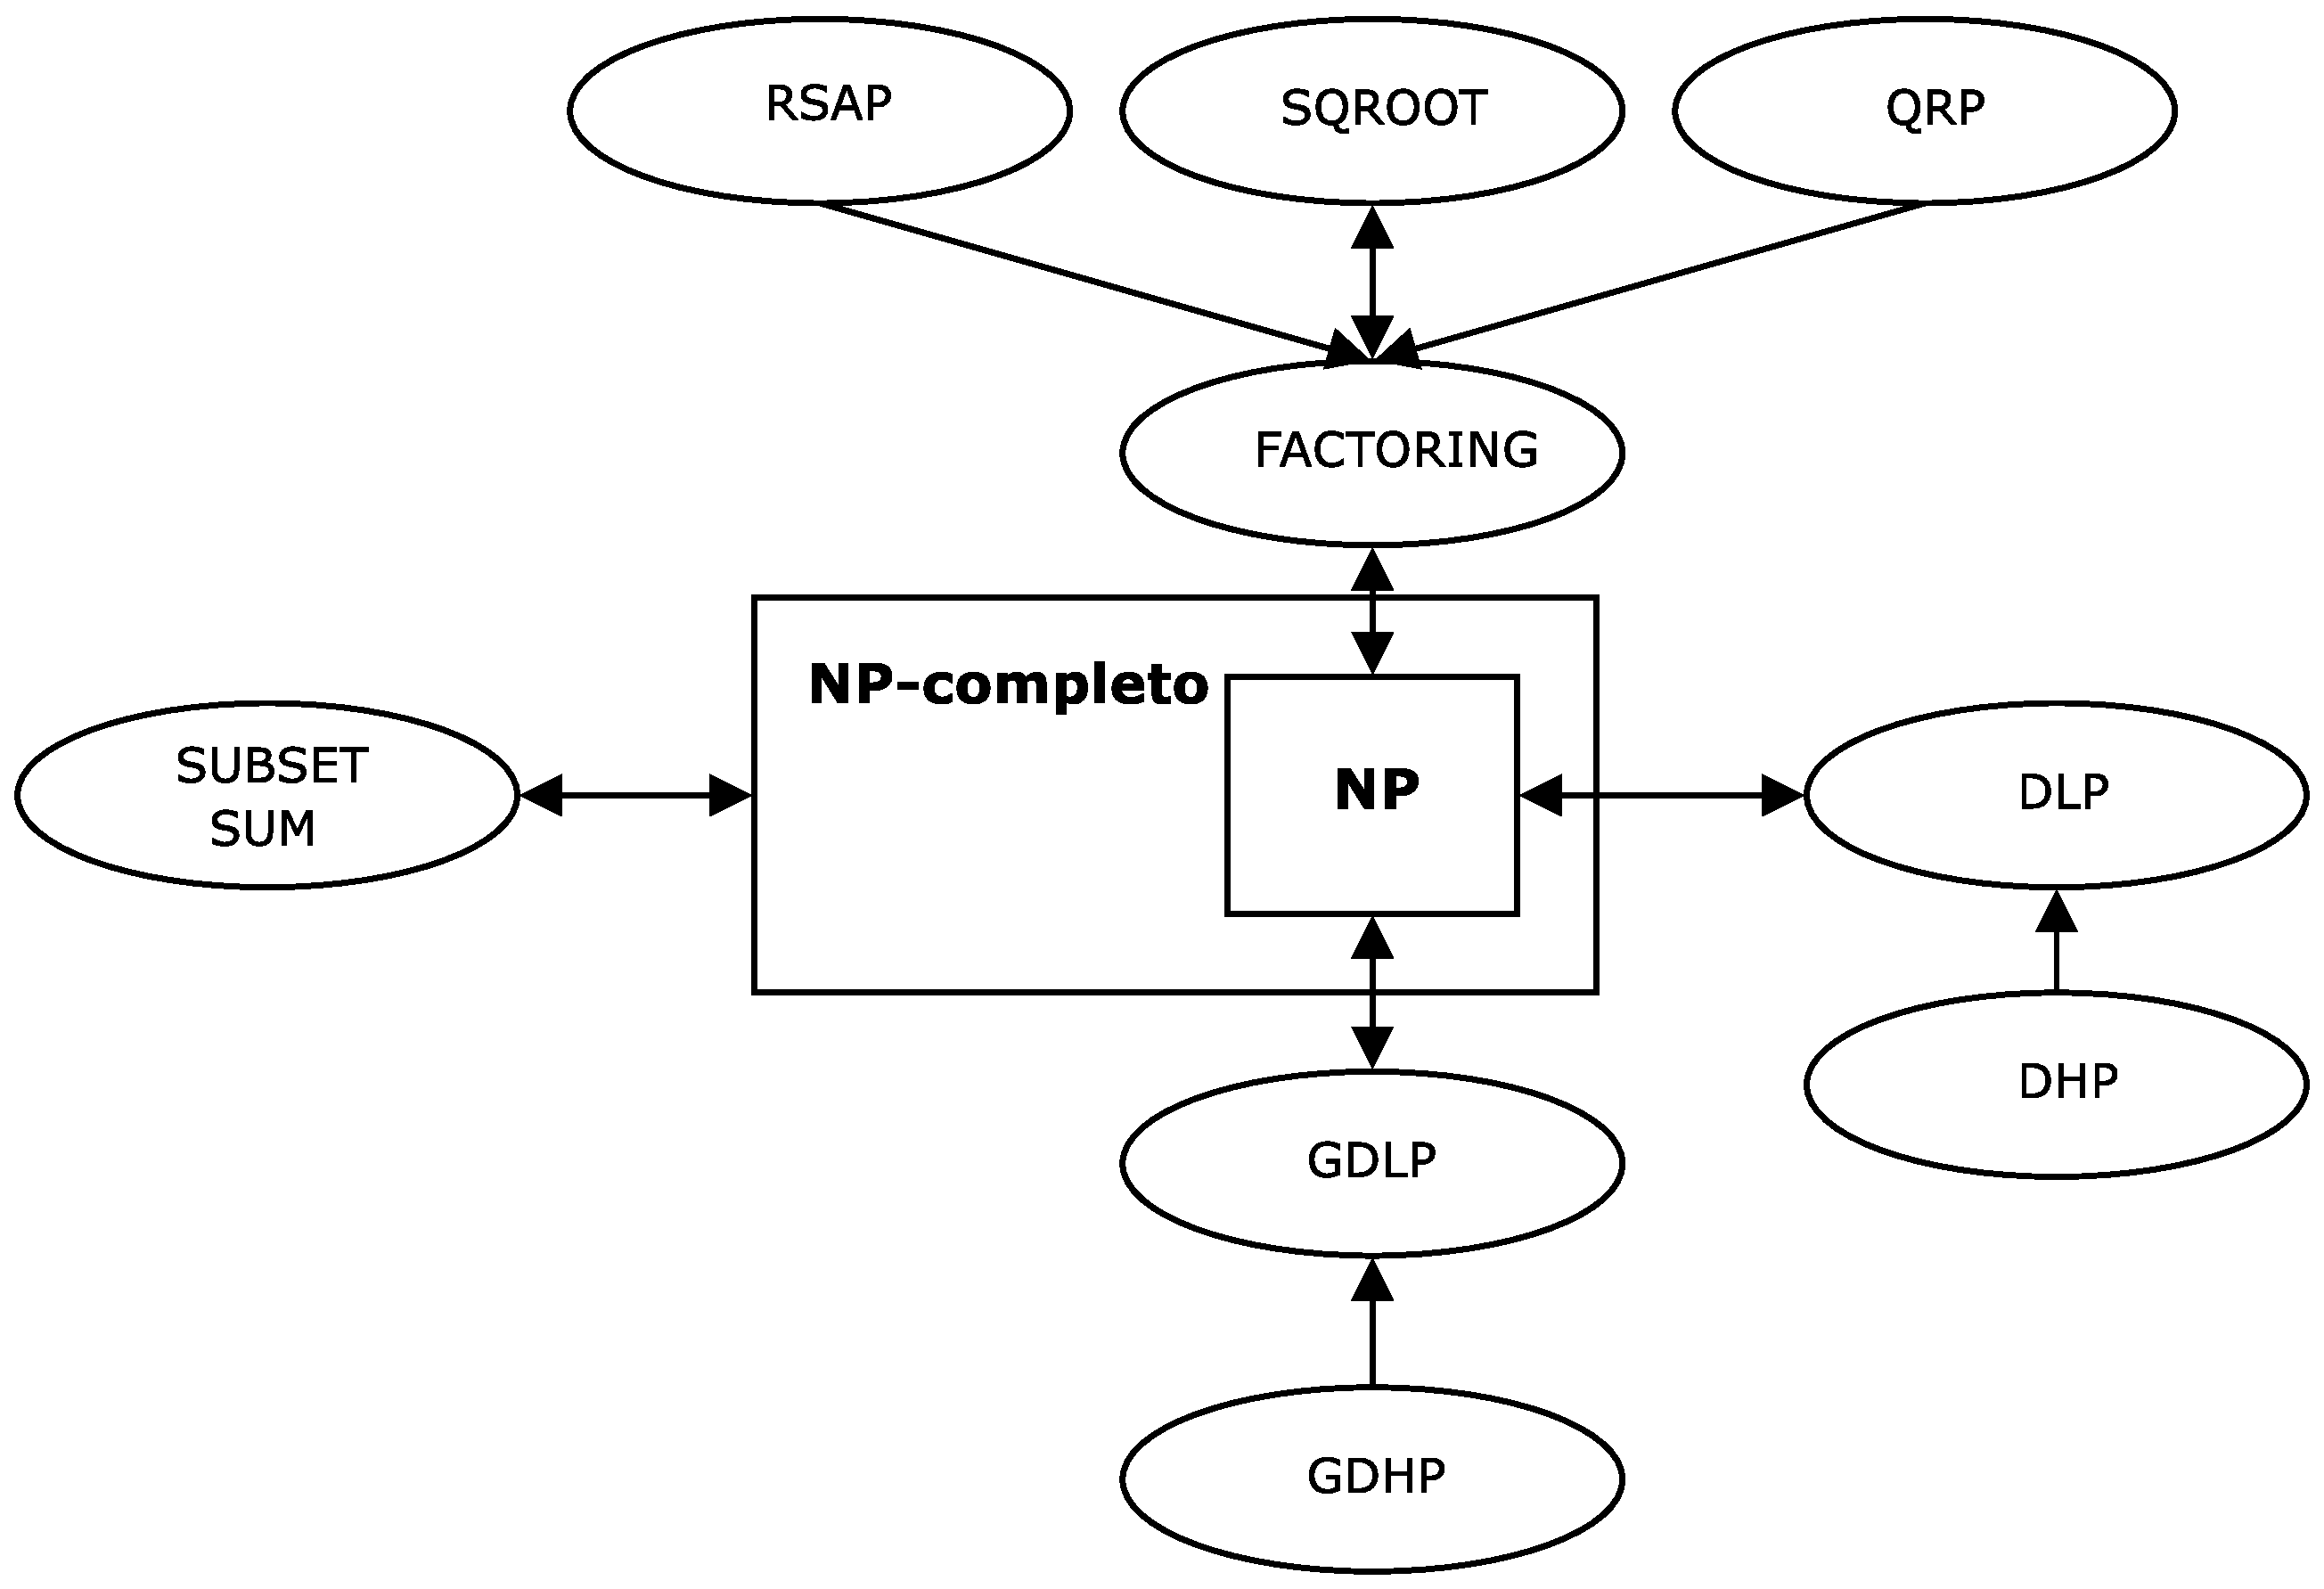
\includegraphics[width=0.9\textwidth,keepaspectratio]
      {problemasFundamentales}
    \end{center}
    \caption{Los problemas fundamentales y sus interrelaciones}
  \end{figure}

  \subsubsection{FACTORING}\label{factoring}
  Uno de los problema fundamentales centrales. A �l se reducen otros
  tres problemas y es por si mismo la base de la gran mayor�a de
  esquemas que utilizan de alg�n modo un problema intratable como base
  de su seguridad. 
  Su formulaci�n rigurosa es la siguiente:
  \begin{definicion}[Problema FACTORING]
    Dado un entero $n$, encontrar su descomposici�n prima. Esto es,
    encontrar los primos de la forma $p_i^{e_i}$ tales que
    $n = \prod_{i=1}^k p_i^{e_i}$.
  \end{definicion}

  El ejemplo cl�sico de algoritmo que se apoya en
  este problema es el m�todo de clave p�blica RSA, en el cual este problema FACTORING
  tiene su representaci�n en el c�lculo de $\phi(n)$ para un entero
  $n$, siendo $\phi$ la funci�n ``totient'' o ``$\phi$ de Euler'',
  cuya definici�n es ``el n�mero de enteros positivos que son coprimos con $n$, 
  considerando que $1$ es coprimo de todo n�mero''. Es evidente que
  $\phi(p) = p - 1$ para $p$ un primo. En base a esto y a la
  descomposici�n prima de $n$ se realiza el c�lculo de $\phi(n)$ para
  un $n$ arbitrario.
  Es m�s, precisamente en el algoritmo RSA se basa el siguiente
  problema fundamental.
  
  \subsubsection{RSAP}\label{rsap}
  Correspondiente al paso fundamental de encriptaci�n del algoritmo
  RSA, pero ``a la inversa'': no
  se trata de conseguir la clave $e$ de un mensaje $m$ determinado,
  sino m�s bien el mensaje $m$ que se corresponder�a con la
  el texto cifrado $c$, habiendo utilizado la clave $e$.
  \begin{definicion}[Inversi�n RSA]
    Dado un entero $n$ producto de dos primos $p$ y $q$, un entero
    positivo $e$ tal que $\gcd(e, (p-1)(q-1)) = 1$ y un entero $c$,
    encontrar un $m$ tal que $m^e \equiv c \pmod{n}$.
  \end{definicion}
  Como se muestra en la figura \ref{fig:problemasFundamentales}, este
  problema se reduce al problema FACTORING.
  
  \subsubsection{SQROOT}\label{sqroot}
    La operaci�n de extraer raices cuadradas m�dulo $p$ con $p$ primo
    es una operaci�n sencilla, como se ve en
    \cite{handbook}\footnote{p�g. 100, algoritmo 3.34}. No lo es, sin
    embargo, cuando el m�dulo reductor es un n�mero compuesto $n$ cuya
    descomposici�n en factores primos se desconoce (y aqu� se intuye
    lo que efectivamente sucede: que este problema se reduce al
    problema FACTORING).

    \begin{definicion}[Ra�ces cuadradas en $\mathbb{Z}_n$]
      Dado un entero $n$ y $a$ un elemento del conjunto de residuos
      cuadr�ticos m�dulo $n$ (v�ase \ref{residuosCuadraticos}),
      encontrar una ra�z cuadrada de $a$
      m�dulo $n$. En s�mbolos, un entero $x$ tal que $x^2 \equiv a
      \pmod{n}$.
    \end{definicion}
  
  \subsubsection{QRP}\label{qrp}
  Con relaci�n a lo que se expone en la secci�n
  \ref{residuosCuadraticos}, es posible formular el siguiente
  problema:
  \begin{definicion}[Problema de los residuos cuadr�ticos]
    Dado un entero impar compuesto,$n$, y un entero $a$ con s�mbolo de
    Jacobi $\left( \frac{a}{n} \right) = 1$, decidir si $a$ es un
    residuo cuadr�tico m�dulo $n$. 
  \end{definicion}
  Si $n$ fuese primo, esto no representar�a un problema, ya que por la
  equaci�n (\ref{calculoLegendre}) de la secci�n
  \ref{simboloLegendre}, el c�lculo ser�a muy sencillo.
  Pero si por contra, $n$ es compuesto, se hace necesaria la
  descomposici�n de $n$ en sus factores primos para realizar el
  c�lculo de los s�mbolos de Legendre correspondientes de la
  definici�n de s�mbolo de Jacobi. Es por esto que se verifica que
  este problema se reduce al problema FACTORING.
  
  \subsubsection{DLP}\label{dlp}
  Este problema es, junto con el problema FACTORING, otro de los
  pilares b�sicos de muchos esquemas de clave p�blica, como por
  ejemplo el sistema de cifrado denominado ElGamal (descrito en
  \cite{handbook}\footnote{pp. 294-298}). Para su definici�n se
  utilizan algunos conceptos de la Teor�a de Cuerpos Finitos que no se
  tratan en esta memoria. En cualquier texto b�sico de Teor�a de N�meros puede 
  encontrarse una definici�n de los mismos, tal como \cite{lidl}.
  \begin{definicion}[Problema de los logaritmos discretos]
    Dado un primo $p$, un generador $\alpha$ de $\mathbb{Z}_p^*$ y un
    elemento $\beta \in \mathbb{Z}_p^*$, encontrar el entero $0 \leq x \leq p-2$ tal
    que $\alpha^x \equiv \beta \pmod{p}$.
  \end{definicion}

  Existe una generalizaci�n de este problema, que responde como se
  pod�a esperar, a las siglas GDLP.
  \begin{definicion}[Problema de los logaritmos discretos generalizado]
    Dado un primo grupo c�clico finito $G$ de orden $n$, un generador $\alpha$ de 
    $G$ y un elemento $\beta \in G$, encontrar el entero $0 \leq x \leq n-1$ tal
    que $\alpha^x = \beta$.
  \end{definicion}

  M�todos y m�s informaci�n al respecto de estos problemas pueden
  encontrarse en \cite{handbook}\footnote{pp. 103-113}.

  \subsubsection{DHP}\label{dhp}
  Un problema �ntimamente relacionado con el problema de los
  logaritmos discretos es el denominado problema de Diffie-Hellman
  \footnote{Quienes, como se expone en la secci�n \ref{clavePublica}, 
  son dos de los padres de la criptograf�a de clave p�blica.}.
  
  N�tense las grandes similitudes en la definici�n:
  \begin{definicion}[Problema de Diffie-Hellman]
    Dado un primo $p$, un generador $\alpha$ de $\mathbb{Z}_p^*$ y 
    elementos $\alpha^a \bmod p$ y $\alpha^b \bmod p$, encontrar 
    $\alpha^{ab} \bmod p$.
  \end{definicion}

  Siguiendo con las similitudes, de este problema tambi�n existe una
  generalizaci�n:
  \begin{definicion}[Problema de Diffie-Hellman generalizado]
    Dado grupo c�clico finito $G$, un generador $\alpha$ de $G$ y
    elementos $\alpha^a \bmod p$ y $\alpha^b \bmod p$ de dicho grupo, encontrar 
    $\alpha^{ab}$. 
  \end{definicion}

  El parentesco entre el problema de los logaritmos discretos y el
  presente problema de Diffie-Hellman se remata con sendas reducciones
  entrelazadas: el problema de Diffie-Hellman (DHP) se reduce al problema de 
  los logaritmos discretos (DLP) y el problema de Diffie-Hellman
  generalizado se reduce al problema de los logaritmos discretos
  generalizado, como se recoge en la figura
  \ref{fig:problemasFundamentales}.

  \subsubsection{SUBSET SUM}\label{subsetSum}
  Este problema tiene una caracter�stica particular, y es que se trata
  de un problema perteneciente a la clase de complejidad
  \textbf{NP-completo} (v�ase \ref{clasesDeComplejidad}). 
  
  \begin{definicion}[Problema de la suma del subconjunto]
    Dado un conjunto de enteros positivos $A={a_1,a_2,\cdots,a_n}$ y un
    entero positivo $s$, determinar si existe un subconjunto de $A$
    tal que sume $s$.
  \end{definicion}

  N�tese que esto \emph{no} es lo mismo que el conocido
  \index{problema!de la mochila}{``problema de
  la mochila''}. Tal problema s�lo es un caso particular del problema
  SUBSET SUM.
 
  M�todos y m�s informaci�n al respecto de este problema puede
  encontrarse en \cite{handbook}\footnote{pp. 117-122}.
  
\section{Teor�a de N�meros}
    En esta secci�n se recogen algunos viejos conocidos de nuestras
    etapas escolares y otras construcciones quiz�s no tan usuales. En
    cualquier caso, forman el \textit{sine qua non} de cualquier
    trabajo en criptograf�a.
    
    \subsection{Euclides y el teorema fundamental de la Aritm�tica}
    \label{teoremaFundamentalAritmetica}
    El c�lebre ge�metra griego Euclides (nacido alrededor del 330
    a.C.) recogi� en su obra \textit{Los Elementos} 465
    proposiciones, que divididas en trece
    ``libros''\footnote{t�rmino arcaico para ``cap�tulos''} han
    constituido el libro de texto de mayor �xito de la historia,
    habiendo sido hasta el siglo XX ``la obra m�s importante del
    mundo despu�s de la Biblia'' (\cite{fermat}\footnote{p�g. 63}).
    Una de estas proposiciones se enuncia a continuaci�n, con un
    \emph{important�simo} corolario que de ella se desprende.
  
    \begin{teorema}[Principio de Euclides]
      Sean $a$ y $b$ enteros y sea $p$ un primo tal que $p | ab$.
      Entonces, $p | a$ � $p | b$.
    \end{teorema}
    \begin{corolario}[Teorema fundamental de la Aritm�tica]
      Cualquier $n \in \mathbb{Z}_0$ puede ser escrito \emph{de forma
      �nica} como un producto de primos.
    \end{corolario}
    
    As�, se podr�a entender todo elemento $n \in \mathbb{Z}_0$ como 
    $2^{e_1} \times 3^{e_3} \times 5^{e_5} \times \cdots \times
    p_k^{e_{p_k}} \times \cdots$, donde los exponentes $e$ ser�an $0$ salvo para un
    n�mero finito de casos.
   
    Parece adecuado apuntar aqu� una anecdota al respecto de
    Euclides, y m�s en unos tiempos tan pragm�ticos ---por llamarlos
    de alguna manera--- como los que corren. En una ocasi�n, uno de
    los alumnos de Euclides le pregunt� acerca de la utilidad de
    aquello que estaba aprendiendo; Euclides se volvi� hacia �l y
    dijo: ``Dad una moneda al muchacho si lo que quiere es sacar
    provecho de todo lo que aprende''. 
    
    \subsection{\index{M�ximo com�n divisor}{M�ximo com�n divisor}}
    \label{maximoComunDivisor}
      Un concepto omnipresente, tratado desde la escuela y
      representado tras la definici�n que muchos aprendimos bajo la
      forma de la letan�a \begin{quotation}``El m�ximo com�n divisor es el mayor de los
      divisores comunes''\end{quotation} que por evidente resultaba in�til. Tambi�n
      se grababa a fuego c�mo calcular dicho m�ximo, 
      \begin{quotation}``multiplicando la menor 
      potencia de cada factor com�n''.\end{quotation} As� es que parece
      que para calcular esta funci�n se hace necesario conocer la
      descomposici�n prima de los n�meros en cuesti�n, o eso parec�a
      cuando las cosas se aprend�an mediante retah�las.
      Muy posiblemente el lector ya sabe que esto no es as�, desde
      hace cientos ($22.5$ ``cientos'' aproximadamente) 
      de a�os se sabe: Euclides recog�a tamb�en en \textit{Los Elementos}
      una manera de calcular el m�ximo com�n divisor de dos enteros sin necesidad de
      disponer de su descomposici�n en factores primos. Se muestra
      esta manera, casi con toda seguridad el algoritmo m�s citado de la
      Historia, en el algoritmo \ref{alg:euclides}. En
      \cite{knuth2}\footnote{p�g. 318} puede leerse incluso una
      reproducci�n cuasi-textual del texto original de Euclides.
      \begin{algorithm}
        \caption{Algoritmo de Euclides del m�ximo com�n divisor}\label{alg:euclides}
        \begin{algorithmic}[1]
          \Procedure{Euclides}{entero $a$, entero $b$}
          \Require $(a \geq 0) \wedge (b \geq 0) \wedge ((a \neq 0)
          \vee (b \neq 0))$
            \Comment Si $a$ � $b$ son negativos, apliquese el
            algoritmo al valor absoluto del n�mero que corresponda,
            por lo recogido en las observaciones \ref{observacionesGCD}.
          
          \While{$b \neq 0$}
            \State $resto \gets (a \bmod b)$
            \State $a \gets b$
            \State $b \gets resto$
          \EndWhile
          \State \Comment Aqu�, $b = 0$.
          \State \textbf{devolver} $a$
         
          \EndProcedure
        \end{algorithmic}
      \end{algorithm}

      Finalmente, resta dar una definici�n formal:
      \begin{definicion}[M�ximo com�n divisor]
        Sean $a$ y $b$ enteros con al menos uno de ellos distinto de
        $0$. Se dice que su \emph{m�ximo com�n divisor}, $d$, es el mayor
        entero que divide simult�neamente a $a$ y $b$.
      \end{definicion}
      
      V�anse algunas de las propiedades que se desprenden de esta
      definici�n.
      \begin{observacion}\label{observacionesGCD}
        Sean $a$ y $b$ enteros y $d$ su m�ximo com�n divisor. Esto se
        representar� como $d = \gcd(a,b)$, respetando las siglas
        inglesas ``Greater Common Divisor'', m�s extendidas en la
        bibliograf�a.
        \begin{itemize}
          \item $d$ es el �nico entero
            divisible a su vez entre cualquier otro n�mero que divida
            simult�neamente a $a$ y $b$.
          \item Por lo expuesto en la secci�n
            \ref{teoremaFundamentalAritmetica}, 
            $d = \prod_{p\; \textrm{primo}} p^{\min(a_p, b_p)}$.
          \item $\gcd(0,0) = 0$ por convenio.\\*
                $\gcd(a,b) = \gcd(b,a)$ \\*
                $\gcd(a,b) = \gcd(-a,b)$ \\*
                $\gcd(a,0) = |a|$
        \end{itemize}
      \end{observacion}

      \subsubsection{El c�lculo ``extendido''}\label{gcdExtendido}
        El t�rmino ``extendido'' se refiere a la obtenci�n no solo de
        $d$, el valor del m�ximo com�n divisor, sino tambi�n de los
        factores que acompa�ar�an, en combinaci�n lineal, a $a$ y $b$. 
        En s�mbolos (\cite{koblitz}\footnote{p�g. 14, I.2.2}):
        \begin{teorema}
          Sean $a$ y $b$ enteros y $d$ su m�ximo com�n divisor. Sin
          p�rdida de generalidad, sea $a > b$. Entonces, existe dos
          enteros $C$ y $D$ tales que $d = Ca + Db$.
        \end{teorema}
        
        Esto es de enorme utilidad, siendo la obtenci�n
        de $C$ y $D$ fundamental para, por ejemplo, el c�lculo de
        inversas (cuando sea posible) en anillos como $\mathbb{Z}_n$. 
        Tambi�n, claro est�, para cuerpos $\mathbb{Z}_p$ con $p$
        primo.

       
        Por �ltimo, como suele ser habitual, \cite{knuth2} es una
        referencia b�sica tambi�n para esta funci�n. Toda su secci�n
        4.5.2 (21 p�ginas) la dedica an�lisis exhaustivo del m�ximo
        com�n divisor.
        
    \subsection{M�nimo com�n m�ltiplo}\label{minimoComunMultiplo}
    Un concepto muy emparentado al de m�ximo com�n divisor es el de
    m�nimo com�n m�ltiplo. Pr�cticamente todas las an�cdotas que
    anteriormente se aplicaron al m�ximo com�n divisor se pueden
    trasladar tambi�n a este caso. 
 
    \begin{definicion}[M�nimo com�n m�ltiplo]
      Sean $a$ y $b$ enteros. Se dice que su 
      \emph{m�nimo com�n m�ltiplo},$l$, es el menor
      entero que $a$ y $b$ dividen.
    \end{definicion}

    Y tambi�n se comparte una formulaci�n muy similar:
    $l = \prod_{p\; \textrm{primo}} p^{\max(a_p, b_p)}$.

    Es f�cil ver las fuertes relaciones entre estos dos conceptos de
    m�ximo com�n divisor y m�nimo com�n m�ltiplo, y extrayendo
    las siguientes relaciones (``m�ximo com�n divisor'' se representar�,
    al igual que anteriormente, como $\gcd(a,b)$, mientras que el m�nimo 
    com�n multiplo ser� representado como $\textrm{lcm}(a,b)$, respetando las 
    siglas inglesas ``Least Common Multiple'', m�s extendidas en la
    bibliograf�a):

    \begin{eqnarray}
      \textrm{lcm}(a,b) & =  &\frac{|ab|}{\gcd(a,b)} \label{lcm-gcd}\\
      \gcd(\textrm{lcm}(a,b),\textrm{lcm}(a,c)) & = & \textrm{lcm}(a, \gcd(b,c)) \\
      \textrm{lcm}(\gcd(a,b),\gcd(a,c)) & =  & \gcd(a, \textrm{lcm}(b,c)) 
    \end{eqnarray}

    Mediante la relaci�n (\ref{lcm-gcd}) el c�lculo del m�nimo com�n
    m�ltiplo se reduce a la del m�ximo com�n divisor m�s un producto y
    una divisi�n.
      
    \subsection{Congruencias}\label{congruencias}
  A modo de referencia, se recoge aqu� la definici�n y un peque�o resumen de las
  propiedades del concepto de ``congruencia''.

  \begin{definicion}
    Dados tres enteros $a$, $b$ y $m$, se dice que ``$a$ es congruente
    con $b$ m�dulo $m$'' y se escribe $a \equiv b \pmod{m}$, si
    $(a-b)$ es divisible entre $m$.
  \end{definicion}
  Otra forma de verlo es comprobar si el resto de las divisiones enteras 
  $\lfloor (a/m) \rfloor$ y  $\lfloor (b/m) \rfloor$ coinciden.

  Se satisfacen las siguientes propiedades:
  \begin{eqnarray}
    a \equiv a \pmod{m} & & \label{cong1} \\ 
    a \equiv b \pmod{m} & \Leftrightarrow & b \equiv a \pmod{m}  \label{cong2} \\
    a \equiv a \pmod{m} \wedge b \equiv c \pmod{m} & \Rightarrow & a \equiv c \pmod{m}  \label{cong3} \\
    a \equiv b \pmod{m} \wedge c \equiv d \pmod{m} & \Rightarrow & a \pm c \equiv b \pm d \pmod{m}  \label{cong4} \\
    a \equiv b \pmod{m} \wedge c \equiv d \pmod{m} & \Rightarrow & ac \equiv bd \pmod{m}  \label{cong5}\\
    a \equiv b \pmod{m} & \Rightarrow & a \equiv b \pmod{d}
    \textrm{ si $d | m$}   \label{cong6}\\
    a \equiv b \pmod{m} \wedge a \equiv b \pmod{n}  &
    \Rightarrow & a \equiv b \pmod{mn} \textrm{ si $\gcd(m,n)=1$}  \label{cong7}
  \end{eqnarray}
  
  Las propiedades (\ref{cong1}), (\ref{cong2}) y (\ref{cong3}) indican
  que la congruencia es una \emph{relaci�n de equivalencia}.
  Las propiedades (\ref{cong4}) y (\ref{cong5}) por su parte indican
  que $\mathbb{Z}_m$ tiene estructura de \emph{anillo conmutativo}.
  
  \subsection{Residuos cuadr�ticos}\label{residuosCuadraticos}
  Concepto que aparece con frecuencia en el trabajo con Teor�a de
  N�meros, en conceptos como tests de composici�n y factorizaci�n, por
  poner dos ejemplos.
  \begin{definicion}[Residuo cuadr�tico]
  Sea $p$ un primo y $0 < a < p$. Entonces $a$ es un \emph{residuo
  cuadr�tico} m�dulo $p$ si se verifica $x^2 \equiv a \pmod{p}$ para
  alg�n $x$.
  \end{definicion}
  Para un m�dulo $n$ arbitrario, no necesariamente primo, tendr�a que
  verificarse que $a$ cumple la anterior definici�n para todo factor
  de la descomposici�n prima de $n$.

  En las siguientes secciones se presentan tres conceptos relacionados
  con los residuos cuadr�ticos. Se presentan tan s�lo las definiciones
  b�sicas y algunas propiedades interesantes de las muchas que estos
  s�mbolos tienen, por lo que se remite al lector interesado a
  \cite{cohen}\footnote{pp. 27-31}, \cite{riesel}\footnote{pp.
  278-288}.
    \subsubsection{S�mbolo de Legendre}\label{simboloLegendre}
    Para la constataci�n del car�cter de residuo cuadr�tico o no de un
    n�mero respecto a un m�dulo primo, se cuenta con el denominado
    \index{s�mbolo!de Legendre}{s�mbolo de Legendre}.
    \begin{definicion}[S�mbolo de Legendre]
      El s�mbolo de Legendre $\left( \frac{a}{p} \right)$, con $p > 2$ un
      primo, se define como:
      \[
        \left( \frac{a}{p} \right) = \left\{ 
        \begin{array}{ll}
          0 & \textrm{si $p|a$} \\
          1 & \textrm{si $a$ es un residuo cuadr�tico m�dulo $p$} \\
          -1 & \textrm{si $a$ es un residuo no cuadr�tico m�dulo $p$}
        \end{array}
        \right.
      \]
    \end{definicion}
    Dos propiedades muy importantes de este s�mbolo son las
    siguientes:
    \begin{observacion}[Multiplicabilidad]
    Se verifica
      \[    
          \left( \frac{a}{p} \right) \times \left( \frac{b}{p} \right) =
          \left( \frac{ab}{p} \right)
      \]
    \end{observacion}

    Y como ayuda a la hora del c�lculo del s�mbolo, se cuenta con la
    siguiente congruencia:
    \begin{equation}\label{calculoLegendre}
      a^{(p-1)/2} \equiv \left( \frac{a}{p} \right) \pmod{p}
    \end{equation}
    
    \subsubsection{S�mbolo de Jacobi}\label{simboloJacobi}
    Como generalizaci�n del s�mbolo de Legendre para los impares
    positivos (no necesariamente primos), se tiene el denominado
    \index{s�mbolo!de Jacobi}{s�mbolo de Jacobi}:
    \begin{definicion}[S�mbolo de Jacobi]
      El s�mbolo de Jacobi $\left( \frac{a}{n} \right)$, con $n > 0$ impar,
      se define como:
      \[
      \left( \frac{a}{n} \right) = 
         \left(\frac{a}{n_1}\right)^{e_1} \left(\frac{a}{n_2}\right)^{e_2} 
         \cdots \left(\frac{a}{n_k}\right)^{e_k}
      \]
      para 
      $n = n_1^{e_1} n_2^{e_2} \cdots n_k^{e_k}$ la descomposici�n en
      factores primos de $n$, siendo por tanto $\left(\frac{a}{n_i}\right)$ 
      un s�mbolo de Legendre.
    \end{definicion}
    \subsubsection{S�mbolo de Kronecker}\label{simboloKronecker}
    El \index{s�mbolo!de Kronecker}{s�mbolo de Kronecker} es una
    extensi�n del s�mbolo de Jacobi a todos los enteros. La simbolog�a
    sigue siendo la misma.

    \begin{definicion}[S�mbolo de Kronecker]
      Sean $a$, $b$, $c$ y $d$ enteros. Mediante el uso del s�mbolo de
      Jacobi, se define en general el s�mbolo de Kronecker $\left( \frac{ab}{cd} \right)$ como:
      \[
        \left( \frac{ab}{cd} \right) =  \left( \frac{a}{cd} \right) \left( \frac{b}{cd} \right) =
        \left( \frac{ab}{c} \right) \left( \frac{ab}{d} \right) = 
\left( \frac{a}{c} \right) \left( \frac{b}{c} \right) \left( \frac{a}{d} \right) \left( \frac{b}{d} \right)
      \]
      Para el caso en el que el m�dulo es $-1$ � $2$, se tiene
      respectivamente:
      \[
        \left( \frac{a}{-1} \right) = \left\{ 
        \begin{array}{ll}
          -1 & \textrm{para $a < 0$} \\
          1 &  \textrm{para $a > 0$}
        \end{array}
        \right.
      \]
      
      \bigskip

      \[
        \left( \frac{a}{2} \right) = \left\{ 
        \begin{array}{ll}
          0 & \textrm{para $a$ par} \\
          1 & \textrm{para $a$ impar y $a \equiv \pm1 \pmod{8}$} \\
          -1 & \textrm{para $a$ impar y $a \equiv \pm3 \pmod{8}$} \\
        \end{array}
        \right.
      \]

      En los que el m�dulo es primo
      impar, el s�mbolo de Kronecker se reduce a un \index{s�mbolo!de
      Legendre}{s�mbolo de Legendre}.

    \end{definicion}

  


%% CAPITULO SOBRE LOS FUNDAMENTOS CRIPTOGR�FICOS

\chapter{Fundamentos
criptogr�ficos}\label{cap:fundamentosCriptograficos}

\begin{flushright}
  \begin{minipage}[t]{13cm}
    \begin{flushright}
      \begin{quote}
        \emph{
        Why should you care if you have nothing to hide? 
        }
        \begin{flushright}
          \textbf{\textemdash J. Edgar Hoover}
        \end{flushright}
      \end{quote}
    \end{flushright}
  \end{minipage}
\end{flushright}

\bigskip

\begin{flushright}
  \begin{minipage}[t]{13cm}
    \begin{flushright}
      \begin{quote}
        \emph{
        Quis Custodiet Ipsos Custodes.
        }
        \begin{flushright}
          \textbf{\textemdash Juvenal, circa 128 a.C.}
        \end{flushright}
      \end{quote}
    \end{flushright}
  \end{minipage}
\end{flushright}

\bigskip

\begin{center}{\line(1,0){325}}\end{center}

%--------------------------------------------------------%

\section{Introducci�n}
Ya que la utilidad fundamental de esta librer�a es de ofrecer m�todos
de la Teor�a de N�meros, con la aplicaci�n directa que tienen estos en
criptograf�a, parece adecuado presentar aqu� una peque�a introducci�n
de los conceptos fundamentales de esta disciplina. Por otra parte, se
hace necesario definir algunos conceptos a los que, a lo largo de esta
memoria, se har� referencia.

\section{Los criptosistemas y su clasificaci�n}
Un \index{criptosistema}{\emph{criptosistema}} se define
(\cite{schneier}\footnote{p�g. 4}) como el conjunto de los algoritmos,
las claves posibles y los pares (texto claro)-(texto cifrado)
posibles. En la figura \ref{fig:esquemaCripto} se muestra
esquem�ticamente el proceso de funcionamiento de un determinado
criptosistema, siendo los algoritmos las cajas ``Cifrado'' y
``Descrifrado''; las claves $K$ � las claves p�blicas y privadas de
las partes participantes en la comunicaci�n, $A$ y $B$; y $M$ y $C$ el
par (texto claro)-(texto cifrado). En los apartados siguientes se dar�
una descripci�n m�s precisa, atendiendo al tipo de criptosistema
considerado. Los tipos de criptosistemas considerados han sido los
\index{criptosistema!sim�trico}{\emph{sim�tricos}} y los de 
\index{criptosistema!de clave p�blica}{\emph{clave p�blica}}.

  \begin{figure}\label{fig:esquemaCripto}
    \begin{center}
      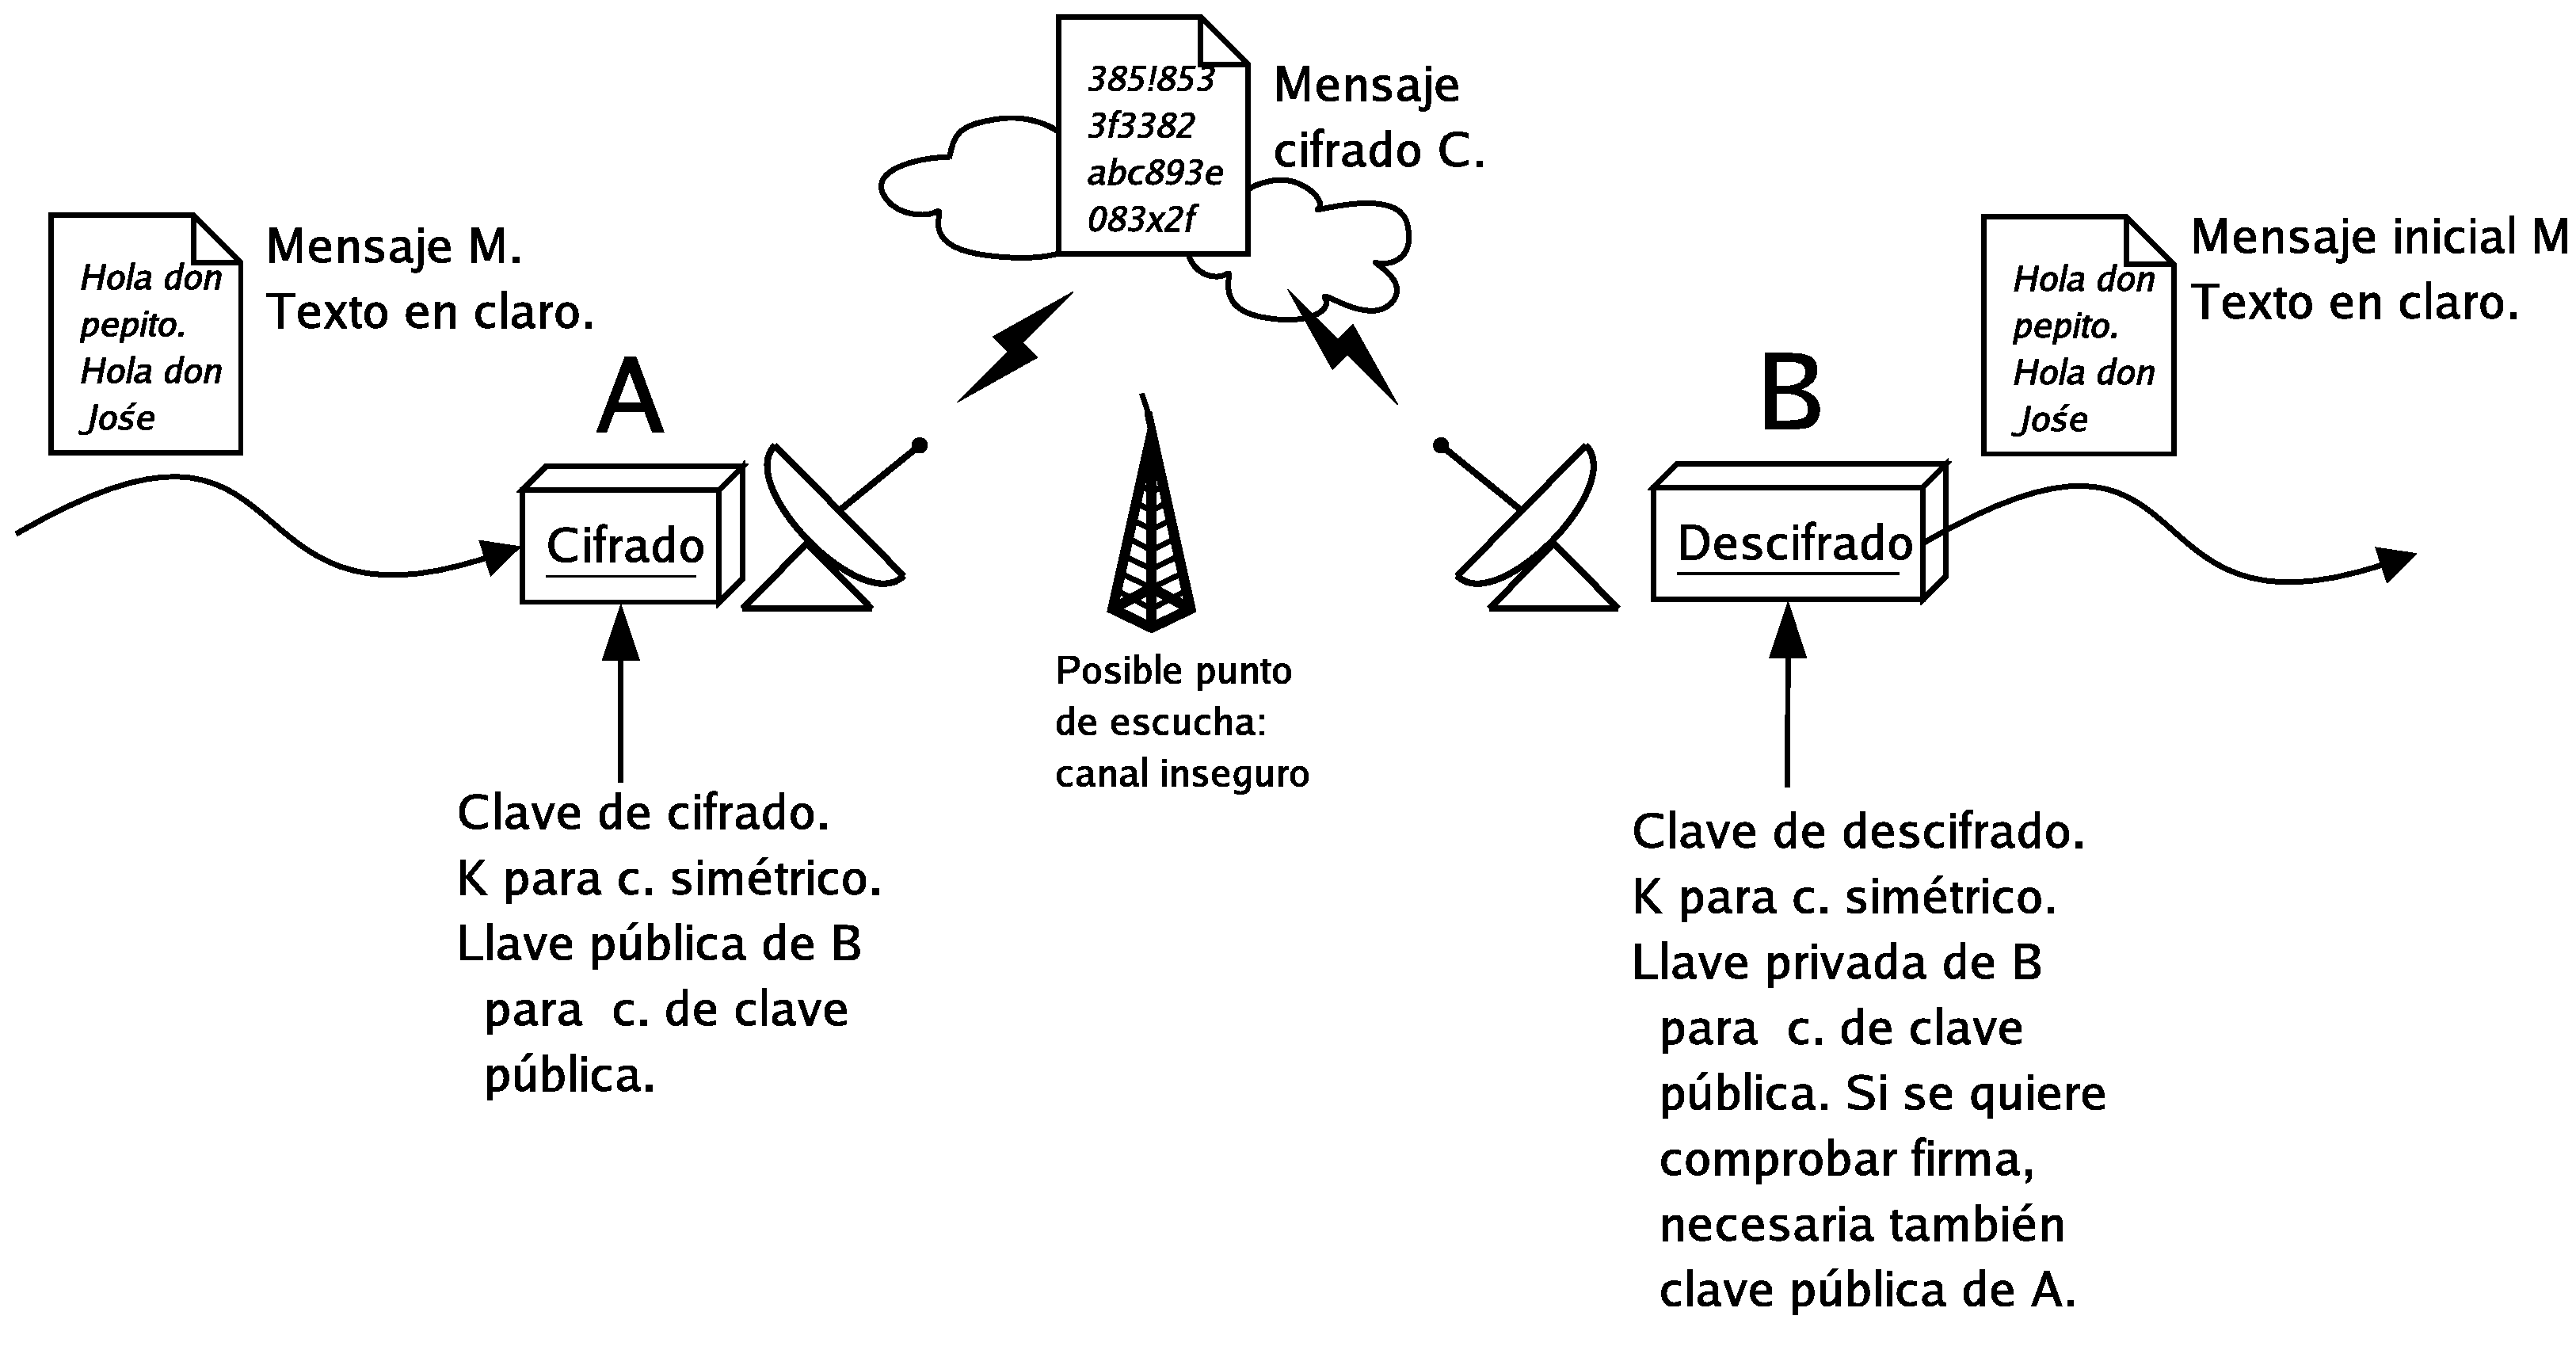
\includegraphics[width=1\textwidth,keepaspectratio]
      {esquemaCripto}
    \end{center}
    \caption{Esquema general de un criptosistema.}
  \end{figure}

  \subsection{Cifrado sim�trico}\label{cifradoSimetrico}
  El esquema ``cl�sico''. Ha sido la forma de utilizar la criptograf�a
  desde la antiguedad\footnote{Cualquiera que haya indagado un poco en
  la historia de la criptograf�a habr� oido hablar del algoritmo de
  cifrado ``Cesar'', el cual se dice que era utilizado por el
  emperador romano Julio Cesar en sus campa�as militares. Los cartaginenses
  deber�an haberse dado
  cuenta de que este m�todo lo �nico que hac�a era desplazar cada
  letra tres posiciones a la derecha en el alfabeto (de forma ``modular'').
  Esto es, de ``a''se pasa a ``d'', de ``y'' a ``b'', etc.}. Su
  caracter�stica distintiva es el utilizar una misma clave\footnote{
  U otra distinta que puede calcularse f�cilmente a partir de �sta.}
  $K$ tanto
  para el proceso de cifrado como para el de descifrado.
  En s�mbolos, siendo $E$ la funcion de cifrado (del ingl�s
  ``Encryption''), $D$ la funci�n de descrifrado, $K$ la clave (del ingl�s ``Key''), $f(k)$ 
  la funci�n de obtenci�n de la clave de descifrado a partir de $K$
  (normalmente suele ser la funci�n identidad),
  $M$ del mensaje en texto claro y $C$ del mensaje cifrado:
  \begin{eqnarray}
    E_k(M) & = & C \\
    D_{f(k)} (C) & = & M 
  \end{eqnarray}
  
  \paragraph{}
    A continuaci�n se da una descripci�n de los
    \index{criptosistemas!modos}{modos} de trabajo posibles de un
    m�todo de cifrado sim�trico. En \cite{schneier} se dedida todo un
    cap�tulo, el noveno, a la descripci�n y comparaci�n entre estos
    modos, y all� se remite al lector interesado en m�s detalles que
    los que aqu� se dan.
    \paragraph{Cifrado de bloques.}\label{cifradoDeBloques}
    El t�rmino ``bloques'' viene de c�mo, esta modalidad de cifrado sim�trico,
    procesa los datos a cifrar. En efecto, los datos son procesados en
    bloques de un tama�o fijo. Habitualmente, se utilizan tama�o del
    orden de 64 bits, lo suficientemente largo para evitar
    vulnerabilidades y lo suficientemente corto para ser manejable
    (\cite{schneier}\footnote{p�g. 4}). Este es el modo de trabajo de,
    por ejemplo, el c�lebre algoritmo DES.
    
    \paragraph{Cifrado de flujo.}\label{cifradoDeFlujo}
    En los m�todos de cifrado sim�trico de flujo, la informaci�n a
    cifrar se va procesando bit a bit, de forma que es posible ir
    arrojando resultados (datos cifrados) de forma pr�cticamente
    simult�nea a su recepci�n, al no tener que esperar a completar
    ning�n tama�o de bloque concreto. Y es precisamente de este hecho
    del que se toma el t�rmino de ``flujo'' (del ingl�s, ``stream'').
    
    Claro, puede pensarse que un cifrado de flujo no es m�s que un
    caso particular de un cifrado de bloques. Efectivamente es as�, y
    es posible transformar algoritmos basados en cada uno de estos
    modos en el otro (sin entrar en si esto tiene alguna utilidad).
    Respecto a esta diferenciaci�n, \cite{schneier}\footnote{p�g. 210}
    cita lo siguiente: 
    \begin{quotation}
      Block ciphers operate on data with a fixed transformation on
      large blocks of plaintext data; stream ciphers operate with a
      time-varying transformation on individual plaintext digits.
    \end{quotation}
    
    Los esquemas de cifrado sim�tricos tienen el problema de la
    distribuci�n de la clave. Si entre los participantes en la
    comunicaci�n, $A$ y $B$ en la figura \ref{fig:esquemaCripto}, no
    existe en alg�n momento una v�a de comunicaci�n segura, no podr�n
    tener la certeza de que sus datos no son capturados y descifrados
    con la clave $K$, la cual un observador malicioso pudo obtener al
    observar la hipot�tica v�a de comunicaci�n insegura que $A$ y $B$
    utilizaron para ponerse de acuerdo en el valor de $K$.
    
    \subsubsection{``One-time pad''}\label{oneTimePad}
     Menci�n aparte merece el m�todo de cifrado denominado ``One-time
     pad'' (quiz�s podr�a traducirse como ``de desplazamiento �nico'',
     pero el t�rmino ingl�s est� lo suficientemente extendido como
     para justificar el no traducirlo). Pese a ser un m�todo de
     cifrado de flujo, se le dedica su propia secci�n por tener el
     car�cter de ``ideal'' respaldado por la teor�a (por la Teor�a de
     la Informaci�n de Claude Shannon en este caso) que, como suele
     ser habitual en estos casos, no es abordable en la pr�ctica. 
     Se describe primero la idea y posteriormente se desvela lo
     especial del m�todo:
     \begin{proposicion}[``One-time pad'']
       La combinaci�n, bit a bit, de una secuencia realmente aleatoria y un
       texto en claro no aleatorio, produce un texto cifrado
       totalmente aleatorio. 
      \end{proposicion}
      \begin{corolario}[Inviolabilidad del ``One-time pad'']
        Un texto cifrado mediante un esquema ``One-time pad'' es
        absoluta y totalmente seguro. 
      \end{corolario}
      La funci�n de combinaci�n puede ser, por ejemplo, una funci�n O
      exclusivo, XOR. De esta forma, es posible, \emph{si se cuenta con la
      secuencia aleatoria utilizada para cifrar}, descifrar el mensaje combinando 
      cada bit del texto cifrado con dicha secuencia.

      Problema: evidentemente, al final estamos igual que al
      principio\ldots la longitud de la clave (la secuencia aleatoria)
      ha de ser la misma que la del texto a cifrar. Entonces, �c�mo
      transmitimos la clave? Si contamos con un canal seguro para
      transmitirla, �por qu� no lo usamos para transmitir directamente
      el mensaje en claro? En cualquier caso, la no utilidad pr�ctica
      de este esquema si sirve, sin embargo, como referente. Los
      esquemas criptogr�ficos reales sacrifican la seguridad total por
      la utilidad: todo lo anterior sirve como un recordatorio de que
      \emph{siempre} existe una posibilidad de que un esquema
      criptogr�fico sea violado. No hay posibilidad de que un esquema
      \emph{�til} sea absolutamente seguro.
      
  \subsection{Cifrado de clave p�blica}\label{clavePublica}
    Esta forma de cifrado es de reciente aparici�n, si se compara con
    el cifrado sim�trico. Whitfield Diffie y Martin Hellman
  fueron quienes, junto a otro de los grandes ---Ralph Merkle---, 
  sentaron en 1976 las bases de la criptograf�a de clave p�blica.
  Ir�nicamente, Malcolm Williamson del Cuartel General de
  Comunicaciones del gobierno brit�nico, ya hab�a descrito tal esquema
  con anterioridad, pero dicho organismo gubernamental brit�nico no
  permiti� su publicaci�n hasta 1997.

  Su caracter�stica fundamental estriba en que las claves utilizadas
  para el cifrado y el descifrado son diferentes. Pero, al contrario que
  en el caso del cifrado sim�trico, una \emph{no} se deriva f�cilmente de
  la otra. Esta ``asimetr�a'' (este tipo de cifrado se denomina
  tambi�n \index{cifrado!asimetrico}{cifrado asim�trico}) se apoya en
  problemas como los expuestos en \ref{problemasFundamentales}.
  La principal ventaja es que, siempre que una de las claves se
  mantenga en secreto, es posible distribuir libremente la otra,
  solucionando as� el problema de distribuci�n de la clave que se
  presenta en los esquemas de cifrado sim�tricos anteriormente
  tratados.
  A la clave que se distribuye se la denomina
  \index{clave!p�blica}{clave p�blica}, y es utilizada para cifrar los
  mensajes. A la que permanece en secreto se la denomina 
  \index{clave!privada}{clave privada}, y es utilizada para descifrar los
  mensajes (tambi�n para firmarlos. Ve�se
  \cite{schneier}\footnote{Cap�tulo 20.} para un an�lisis de m�todos
  de firma digital con esquemas de clave p�blica).

  El esquema de funcionamiento en s�mbolos, con $E$ la funcion de cifrado (del ingl�s
  ``Encryption''), $D$ la funci�n de descrifrado, $K_p$ la clave 
  p�blica (del ingl�s ``Public Key''), $K_s$ la clave privada (del
  ingl�s ``Secret Key''),
  $M$ del mensaje en texto claro y $C$ del mensaje cifrado:

  \begin{eqnarray}
    E_{K_p}(M) & = & C \\
    D_{K_s}(C) & = & M
  \end{eqnarray}

  Para un proceso de firma, el esquema es el mismo pero utilizando
  $E_{K_s}$ para el cifrado y $D_{K_p}$ para el descifrado.
  
\section{Funciones}
\subsection{\index{funciones!unidireccionales}
{Funciones unidireccionales (``One-way'')}}
  \label{funcionesUnidireccionales}
  Fundamentales en criptograf�a, este tipo de funciones satisfacen el
  ser muy f�ciles de calcular pero muy dif�ciles de invertir.
  \begin{definicion}[Funci�n unidireccional]
    Una funci�n $f:X \longrightarrow Y$ se denomina \emph{funci�n
    unidireccional} si $f(x)$ es ``f�cil'' de computar $\forall{x} \in
    X$ pero para un $y \in Im(f)$ elegido al azar es
    ``computacionalmente inabordable'' el encontrar un $x \in X$ tal
    que $f(x) = y$. (\cite{handbook}\footnote{p�g. 8})
  \end{definicion}
  El difuso t�rmino ``f�cil'' se puede entender como perteneciente a
  la clase de complejidad $\mathbf{P}$ (v�ase
  \ref{teoriaDeLaComplejidad}), mientras que por contra
  ``computacionalmente inabordable'' se corresponder�a a las clases
  distintas a $\mathbf{P}$. Pero aqu� uno se encuentra con que
  precisamente no est� demostrado que $\mathbf{P} \neq \mathbf{NP}$,
  con lo cual estos t�rminos se vuelven a�n m�s difusos.
  
  Ejemplos de estas funciones son la factorizaci�n de enteros. Es muy
  sencillo multiplicar $n = p \times q$ pero extremadamente dif�cil
  obtener $p$ y $q$ del conocimiento de $n$. V�ase \ref{factoring} y el
  c�lculo de logaritmos en cuerpos finitos en \ref{dlp}.
    

  \subsection{\index{funciones!con puerta trasera}{Funciones
  con puerta trasera (``trapdoor'')}}\label{funcionesTrapdoor}
  Tambi�n de gran importancia, son un tipo especial de funciones
  unidireccionales con la caracter�stica extra de que si se conoce un
  determinado dato (si se sabe ``d�nde est� la trampilla''), es
  ``f�cil'' calcular la inversa de la funci�n en cuesti�n.

  El ejemplo m�s famoso se encuentra en el algoritmo RSA: el
  conocimiento de la factorizaci�n de $n$ en los dos primos $p$ y $q$
  proporciona una forma en $\mathbf{P}$ de resolver la expresi�n
  $C^{d} \pmod{n}$, con $d = e^{-1} \pmod{\phi(n)}$ siendo $e$ la
  clave de cifrado, cuyo valor ahora no es relevante. Es claro
  que si tenemos en cuenta que $\phi(n) = (p-1)(q-1)$, todo se reduce
  a una potenciaci�n modular, operaci�n que claramente entra dentro
  de la clase de complejidad $\mathbf{P}$. Se considera indispensable
  el conocimiento de la factorizaci�n de $n$ para el c�lculo en
  $\mathbf{P}$ de $\phi(n)$.
  
  \subsection{\index{funciones!hash}{Funciones
  hash}}\label{funcionesHash}
  Estas funciones, tambi�n denominadas \index{funciones!resumen}
  {\emph{funciones resumen}} (del ingl�s, ``digest''), encuentran
  multitud de aplicaciones en criptograf�a, as� como en muchos 
  otros campos. Esto se explica a la vista de sus propiedades:
  \begin{itemize}
    \item Son funciones unidireccionales.
    \item Su codominio es de tama�o constante y conocido (longitud del
      resumen).
    \item Determinar dos elementos con la misma imagen es
      \emph{dif�cil}\footnote{Inabordable computacionalmente
      con los m�todos del momento. V�ase \ref{teoriaDeLaComplejidad}} (resistencia a colisiones).
    \item La imagen no parece mantener ninguna relaci�n con su
      preimagen: con tan s�lo el cambio de un bit en la preimagen, en
      promedio, la mitad de los bits de la imagen cambian
      (\cite{schneier}\footnote{p�g. 30}).
  \end{itemize}
  En s�mbolos:
  \begin{definicion}[Funci�n Hash]
    Sea $H:\{0,1\}^{n} \longrightarrow \{0,1\}^{m}$ para un $m \in
    \mathbb{N}$ constante, verificando:
    \begin{eqnarray}
      H(M)  \stackrel{\mathbf{P}}{=}  h \quad \textrm{dado } M \label{eq:def1Hash} \\
      H^{-1}(h)  \stackrel{\mathbf{NP}}{=}  M \quad \textrm{dado } h \label{eq:def2Hash} \\
      \textrm{Dado M, obtener }M' / H(M) = H(M') \textrm{ es \textbf{NP}} \label{eq:def3Hash}
    \end{eqnarray}
  \end{definicion}
  
  As� pues, entre las aplicaciones m�s importantes est� la
  verificaci�n de integridad de datos, firma electr�nica,
  criptosistemas de clave p�blica, generaci�n de bits
  pseudo-aleatorios, etc.
  
  \subsubsection{Seguridad de las funciones hash}
  En rigor, no existen pruebas matem�ticas de la existencia de
  funciones unidireccionales (\cite{schneier}\footnote{p�g. 29}):
  se conf�a en el estado actual del
  conocimiento en lo relativo a problemas \emph{dif�ciles} para
  obtener este car�cter de funci�n ``de una sola direcci�n''. Se hace
  necesario por tanto realizar un an�lisis de hasta qu� punto estas
  funciones garantizan la seguridad, o dicho de otro modo, hasta qu�
  punto cumplen con su definici�n.
  \paragraph{El ataque del cumplea�os}\label{ataqueCumple}
  �Cu�ntas personas tenemos que estar en una habitaci�n para que
  compartamos fecha de nacimiento con alguno de los presentes con una
  probabilidad mayor que $\frac{1}{2}$?
  \[
    p(coincidencia) = 1 - \left( \frac{364}{365} \right)^n 
  \]
  Por tanto, 
  \[
    p(coincidencia) \geq (1/2) \Rightarrow n \geq 253
  \]
  �Y cu�ntas para que al menos una pareja comparta esta fecha de
  cumplea�os tambi�n con una probabilidad $\geq \frac{1}{2}$?
  \[
    p(coincidencia) = 1 - \left( \frac{364}{365} \times \frac{363}{365}
    \times \cdots \times \frac{365-n+1}{365} \right) = 1 - \left( \frac{365!}{365^n(365-n)!} \right)
  \]
  As� que, 
  \[
    p(coincidencia) \geq (1/2) \Rightarrow n \geq 23 
  \]

  Realizando una analog�a con las funciones hash, el primer supuesto
  se corresponder�a con probar hasta un total de $2^m$ valores diferentes para
  encontrar una colisi�n (ecuaci�n \ref{eq:def3Hash}). Sin embargo,
  en \cite{handbook}\footnote{p�g. 53} se afirma que cuando $m
  \longrightarrow \infty$, el n�mero esperado de pruebas antes de una colisi�n
  es $\sqrt{\frac{\pi m}{2}}$. Por tanto podemos considerar que si nos
  ce�imos simplemente a encontrar dos mensajes cualesquiera $M$ y $M'$ tales que 
  $H(M) = H(M')$, s�lo se habr� de invocar a la funci�n hash $H$ un n�mero
  $O(\sqrt{m})$ de veces. 
  
  �Con tan s�lo $2^{m/2}$ pruebas se
  encontrar�an $M$ y $M'$, una colisi�n para $H$! As�, se reduce a la
  mitad el espacio de b�squeda. Esto no es m�s que la aplicaci�n del
  segundo caso del cumplea�os.

  Conclusi�n: la longitud $m$ de la cadena resumen ha de ser \emph{el
  doble} 
  de lo que el estado de la tecnolog�a del momento permita explorar
  por fuerza bruta.
  
  Ejemplos de c�mo se puede explotar una colisi�n como esta se
  encuentran en \cite{schneier}\footnote{p�g. 430} y
  \cite{handbook}\footnote{pp. 369-371}.

  \subsubsection{MD5}\label{md5}
  Por omisi�n, esta es la funci�n hash que implementa la librer�a. 
  Sus detalles escapan al �mbito de esta memoria, pudiendo encontrarse
  en \cite{rfc1321} su referencia fundamental, de mano de su autor R.
  Rivest (la ``R'' del algoritmo RSA).

  La implementaci�n sigue el c�digo de referencia de dicho documento.

%% EXPOSICION DE CONCEPTOS BASICOS
\chapter{Conceptos b�sicos}

\begin{flushright}
  \begin{minipage}[t]{13cm}
    \begin{flushright}
      \begin{quote}
        \emph{
          Basic research is what I am doing when I don't know what I am doing.
        }
        \begin{flushright}
          \textbf{\textemdash Wernher von Braun}
        \end{flushright}
      \end{quote}
    \end{flushright}
  \end{minipage}
\end{flushright}

\bigskip

\begin{center}{\line(1,0){325}}\end{center}

%--------------------------------------------------------%

  
\section{Estructura general de la biblioteca}
  
  \subsection{Los procesadores virtuales}

    \paragraph{Perfilado}
      

    \subsubsection{La CPU escalar}

    \subsubsection{La CPU SIMD}\label{basico:cpusimd}
    Existe un tipo de paralelismo que ha estado disponible en procesadores de consumo
    desde hace m�s de una d�cada, cuando en $1997$ Intel introdujo el juego de instrucciones 
    MMX en su familia de procesadores Pentium\footnote{\url{ http://www.intel.com/design/intarch/mmx/mmx.htm }}.
    Este tipo de paralelismo, denominado por las siglas SIMD\footnote{instrucci�n �nica m�ltiples datos, por sus siglas en ingl�s}, 
    se expone en la secci�n \ref{flynn}. Resumiendo, se trata de aplicar una �nica instrucci�n a un conjunto de datos �en bloque�.
    Comp�rese la figura \ref{fig:sinSIMD} con la figura \ref{fig:conSIMD}. En la primera, los datos son tratados secuencialmente de
    una manera que podr�a denominarse �horizontal�. Por contra, en la segunda, se aplica la operaci�n en cuesti�n simult�neamente
    a todos los datos, �verticalmente�.

    \begin{figure}[h]
      \centering
      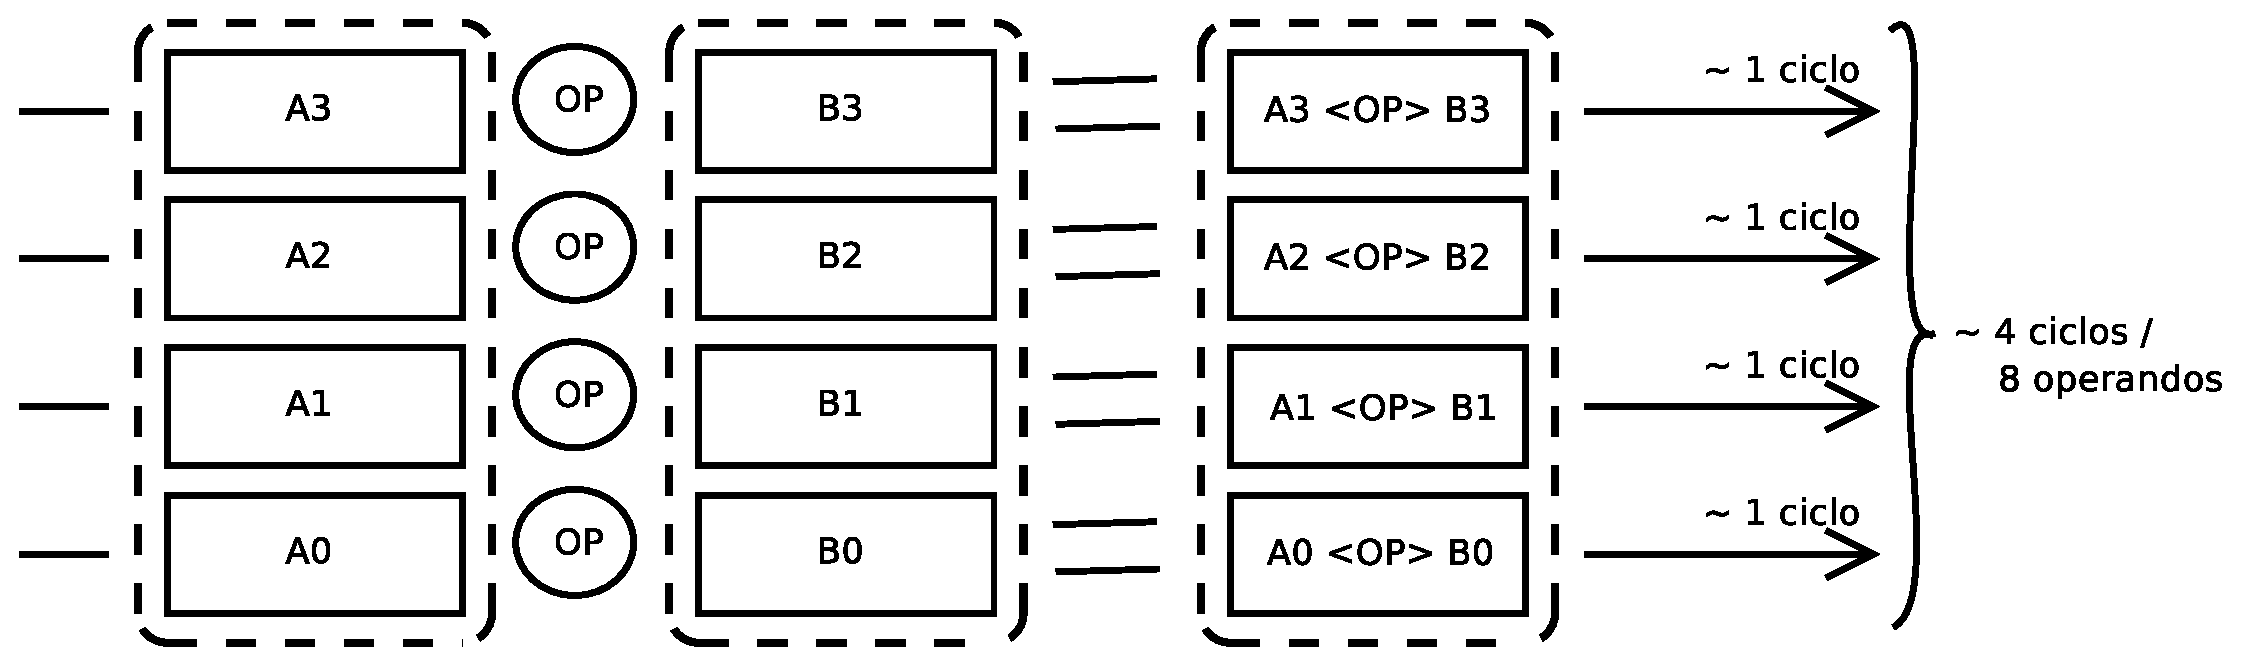
\includegraphics[width=0.85\textwidth,keepaspectratio]{sinSIMD} 
      \caption{Sin utilizar SIMD}\label{fig:sinSIMD}
    \end{figure}

    \begin{figure}[h]
      \centering
      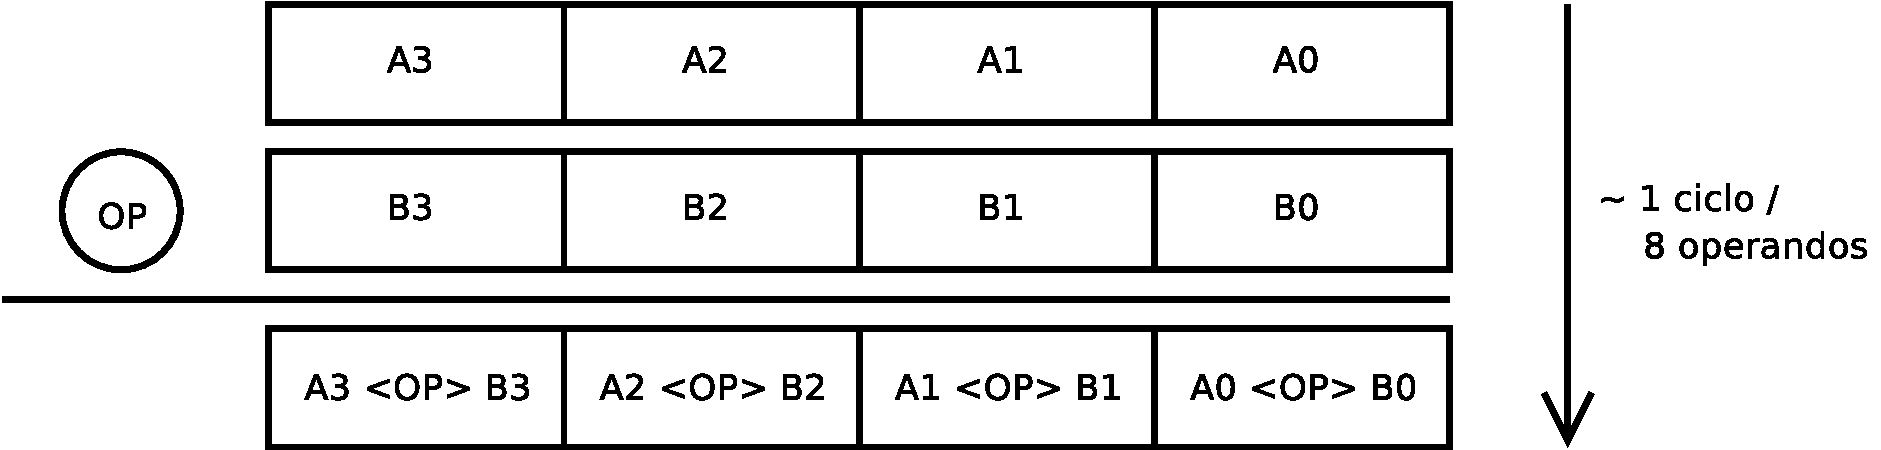
\includegraphics[width=0.85\textwidth,keepaspectratio]{conSIMD} 
      \caption{Utilizando SIMD}\label{fig:conSIMD}
    \end{figure}

    Este paralelismo intr�nseco al procesador requiere el uso de instrucciones espec�ficas del mismo, y es por ello
    dif�cilmente portable a otros sistemas. Asimismo, su utilizaci�n suele requerir el trabajo en lenguaje ensamblador, 
    con todo lo que ello supone (dificultad de mantenimiento, complejidad, etc.).

   La pr�ctica ubicuidad y potencia de estos m�todos los hacen muy atractivos. Con el fin de evitar el obst�culo
   de lo poco amigable de su uso, se ha desarrollado esta �CPU SIMD�. Sus objetivos son:
   \begin{itemize}
      \item Aislar a las rutinas de la biblioteca que deseen hacer uso de instrucciones SIMD de la implementaci�n
      real particular del procesador en cuesti�n sobre el que se est� operando. Incluso si no existe implementaci�n
      alguna, la biblioteca provee una implementaci�n gen�rica que simula su comportamiento.
      \item Homogeneizar la familia de operaciones disponibles, del mismo modo que se ha hecho con la CPU escalar.
      \item Proporcionar una abstracci�n adecuada que evite lidiar con los entresijos del lenguaje ensamblador. 
   \end{itemize} 

   \bigskip 

   Los �paquetes� SIMD tendr�n siempre una longitud de $128$ bits. En base a esto, se han definido
   tres variedades diferentes de �paquetes� de datos SIMD:
   \begin{itemize}
   \item Pares de n�meros en coma flotante de $64$ bits.
   \item Cuatro n�meros en coma flotante de $32$ bits.
   \item Ocho enteros con signo de $16$ bits.
   \end{itemize}
   Los detalles de la implementaci�n y una descripci�n m�s pormenorizada se dan en la secci�n \ref{simddigit}.



  \subsection{Repositorio de funciones}\label{basico:nuevoRepdeFuncs}
Ya en LibNumth exploramos la utilizaci�n de lo que se denomin� �repositorio de funciones�
(v�ase \cite{miproyecto}\footnote{secciones 5.6 y 4.2.3}). La idea era y sigue siendo
�hacer extensible la colecci�n de funciones \emph{sin necesidad de recompilaci�n} por parte del usuario,
y adem�s de forma sencilla�. La implementaci�n de este mecanismo en dicha versi�n de la biblioteca
era un tanto b�sica: depend�a de convenciones en el nombrado, haciendo recaer sobre el usuario
programador la carga de recordar el nombre concreto del tipo de funci�n que desease obtener. Por ejemplo:

\begin{lstlisting}[captionpos=b,basicstyle=\footnotesize,frame=shadowbox,rulesepcolor=\color{black},language=C++,numbers=left,caption=Utilizando el \textbf{antiguo} repositorio de funciones, label=lst:antiguoRepFuncs]
(...)
numth::Funciones funcs;

numth::congruentGen *LCG = new numth::congruentGen();
funcs.ponerRandom(LCG);

funcs.random()->ponerSemilla(numth::Z::convertir("323658476")); 
n = funcs.genPrimos()->leerPrimoProb(600);
(...)
\end{lstlisting}
En el anterior listado \ref{lst:antiguoRepFuncs} se aprecian los siguientes puntos:

\begin{itemize}
\item Tanto para establecer una nueva implementaci�n 
para una clase de m�todo, como para obtener la implementaci�n actual, era necesario estar al tanto del
nombre de la clase de m�todo que las instancias implementaban: \texttt{congruentGen} era un tipo de generador
de n�meros pseudo-aleatorios, y por ello deb�a utilizarse el m�todo \texttt{ponerRandom} de la clase \texttt{Funciones}, 
que representaba el repositorio. 
\item Para obtener un n�mero primo, el programador deb�a recordar que el m�todo
\texttt{genPrimos} era el indicado para obtener un puntero a una instancia generadora de primos. 
\item Incluso aunque se pretend�a seguir un patr�n de nombrado, �ste resultaba deficiente.
\item El repositorio, instancia de la clase \texttt{Funciones}, pod�a instanciarse de forma arbitraria, pese a que
conceptualmente el repositorio ha de ser �nico durante toda la ejecuci�n del programa. Este escollo se salvaba
haciendo que las instancias de las funciones contenidas en �l fueran \texttt{static}. Este simple hecho choca frontalmente
con el concepto de \textit{thread-safety}, tal como se expone en la secci�n \ref{par:datosStatic}.
\end{itemize}

Esta forma de operar no s�lo resulta tediosa y 
propensa a errores, sino tambi�n \emph{poco elegante}. La idea
es siempre que la m�quina trabaje por nosotros, no al contrario. Por si esto fuera poco, la presencia de datos
est�ticos da al traste con las aspiraciones de ejecuci�n concurrente de la biblioteca mediante hilos. 

Comparese el c�digo mostrado en el listado \ref{lst:antiguoRepFuncs} con el mostrado en el siguiente listado \ref{lst:nuevoRepFuncs}:
\begin{lstlisting}[captionpos=b,basicstyle=\footnotesize,frame=shadowbox,rulesepcolor=\color{black},language=C++,numbers=left,caption=Utilizando el \textbf{nuevo} repositorio de funciones, label=lst:nuevoRepFuncs]
(...)
mpplas::MethodsFactory& funcs(MethodsFactory::getReference());
mpplas::RandomFast* rnd;
mpplas::PrimeGen* primes;

mpplas::RandomFast* newRnd = new mpplas::CongruentGen();
funcs.setFunc(newRnd);

funcs.getFunc(rnd);
rnd->setSeed(mpplas::Z("323658476"));

funcs.getFunc(primes);
n = primes->getInteger(600);
(...)
\end{lstlisting}
Ambas porciones de c�digo son sem�nticamente equivalentes. Sin embargo:
\begin{itemize}
\item El repositorio, denominado ahora \texttt{MethodsFactory}, es ahora un \texttt{Singleton} (v�ase secci�n \ref{sec:singleton}). 
\item Se trabaja con punteros a los tipos que representan el concepto \emph{abstracto} a realizar: generar primos, obtener n�meros
pseudo-aleatorios, etc. en vez de con los tipos que en �ltima instancia implementan dichos conceptos.
\item El repositorio consiste \emph{�nicamente} de dos m�todos: \texttt{getFunc} y \texttt{setFunc}. El mecanismo
de funcionamiento, denominado \textit{autowiring}, se expone en \ref{sec:autowiring}. En este contexto, ambos
m�todos inspeccionan el tipo de las instancias que les son pasadas como par�metros a la hora de asignar
o establecer las instancias pertinentes, de forma totalmente transparente para el usuario, y garantizando \emph{en tiempo
de compilaci�n} la coherencia de dichas operaciones.
\end{itemize}

    
  \subsection{Control de errores}\label{controlDeErrores}


\section{Compilando la biblioteca}\label{estructuraGeneralDeLaLiberia}

%% CAPITULO IMPLEMENTACION 

\chapter{Detalles de implementaci�n}\label{chap:detallesImpl}

\begin{flushright}
  \begin{minipage}[t]{13cm}
    \begin{flushright}
      \begin{quote}
        \emph{
          Se deben absorber los colores de la vida, pero nunca deben de
          recordarse sus detalles. Los detalles son siempre vulgares.
        }
        \begin{flushright}
          \textbf{\textemdash Oscar Wilde, El retrato de Dorian Gray}
        \end{flushright}
      \end{quote}
    \end{flushright}
  \end{minipage}
\end{flushright}

\bigskip

\begin{flushright}
  \begin{minipage}[t]{13cm}
    \begin{flushright}
      \begin{quote}
        \emph{
          Cu�date de aquel que no se molesta en los detalles.
        }
        \begin{flushright}
          \textbf{\textemdash William Feather}
        \end{flushright}
      \end{quote}
    \end{flushright}
  \end{minipage}
\end{flushright}

\bigskip

\begin{center}{\line(1,0){325}}\end{center}

%--------------------------------------------------------%
\section{Introducci�n}
 

\section{Elementos generados din�micamente}
 
  - system info
    - cpu info
    - compilation config
  - preprocesador en python
  - el cliente en python
  - el mecanismo de perfilado basado en aop


\section{Asegurando la coherencia algebraica}
- comprobaciones estataticas de caracter algebraico de parametros de templates
en la particularizaci�n de estructuras genericas


\section{El nuevo repositorio de funciones}

\section{Una nueva cpu}
- cpu vectorial


\section{La utilidad de fingir}
- mock openmp


\section{El mundo de los $64$ bits}

\section{El maestro compilador}
- scons

\section{Implementaci�n de tipos}
  \subsection{El tipo \emph{\texttt{MPPDataType}}\index{tipos!MPPDataType} }

  \subsection{Categorizaci�n algebraica}
  En la figura \ref{fig:categoriasAlgebraicas} se muestra la jerarqu�a de clases que
  modelan las categor�as algebraicas consideradas, junto con sus m�todos (est�ticos) asociados.  
  \begin{figure}[h]
    \centering
    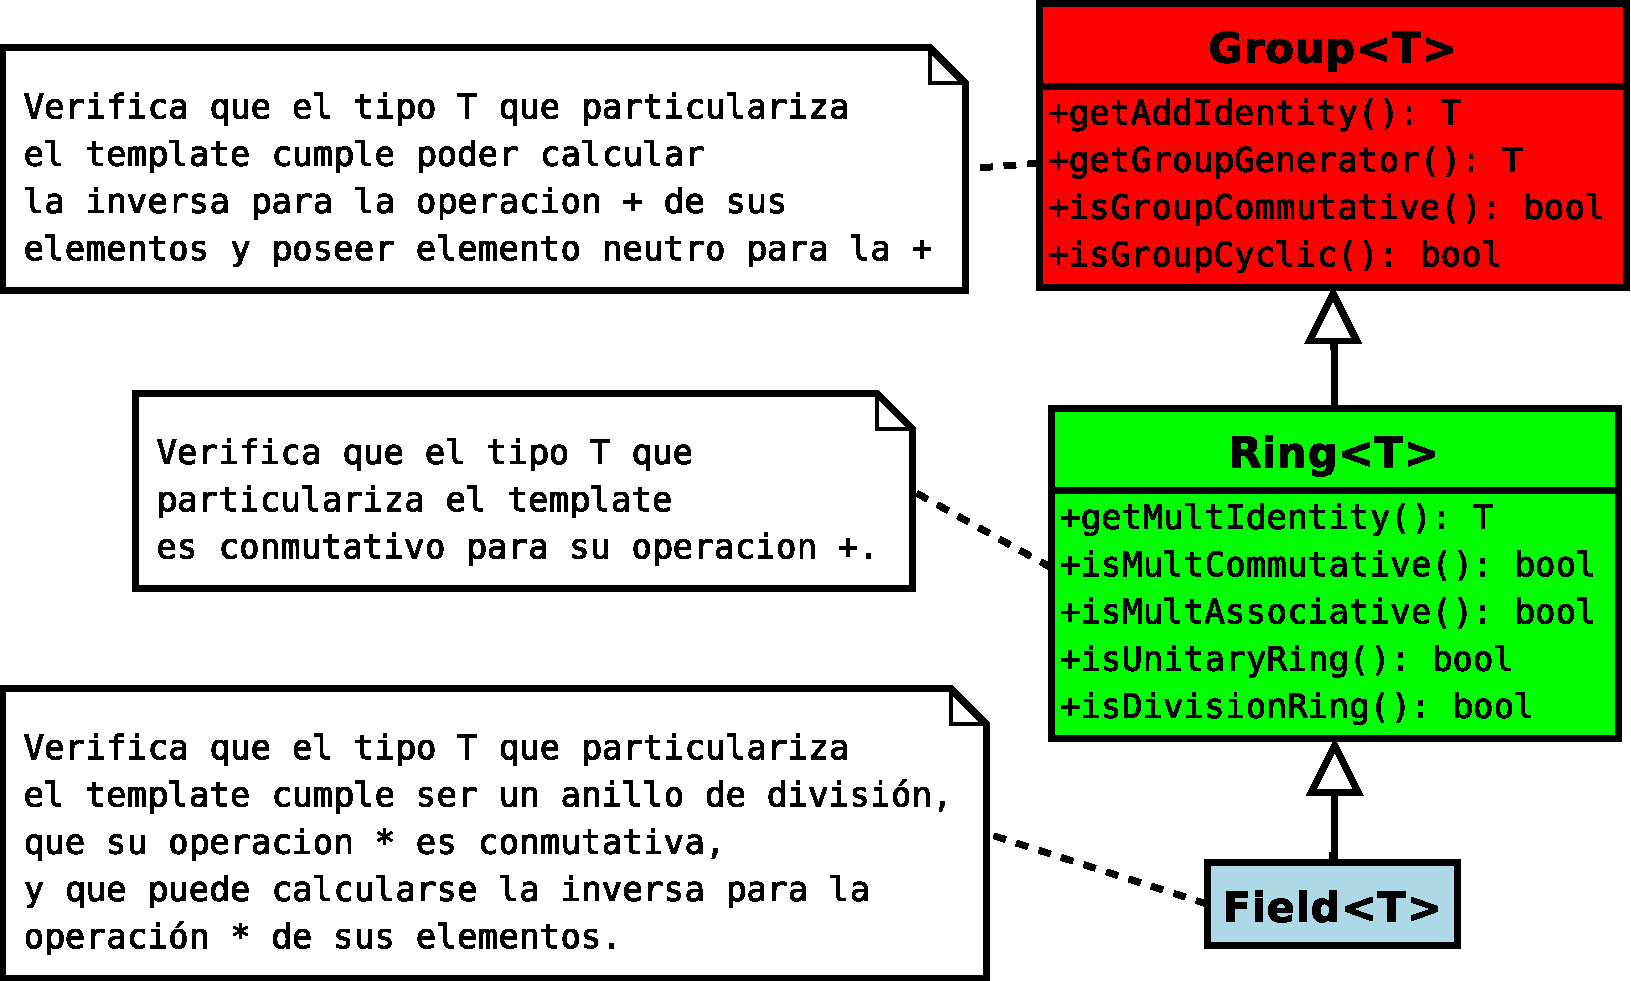
\includegraphics[width=0.95\textwidth,keepaspectratio]{categoriasAlgebraicas} 
    \caption{Categorias algebraicas}\label{fig:categoriasAlgebraicas}
  \end{figure}
  Cuando un tipo de dato de la librar�a (es decir, un hijo de \texttt{MPPDataType}) se
  encasilla dentro de esta jerarqu�a, sobre dicho tipo (representado mediante el par�metro 
  de plantilla \texttt{T}) se realizan una serie de comprobaciones, dise�adas para verificar
  que efectivamente dicho tipo cumple las condiciones impuestas por la categor�a 
  algebraica a la que aspira pertenecer. Esta serie de comprobaciones se realizan por medio
  de \emph{asertos}.



\begin{lstlisting}[captionpos=b,basicstyle=\footnotesize,frame=shadowbox,rulesepcolor=\color{black},language=C++,numbers=left,caption=STATIC\_ASSERT, label=lst:staticassert]
~Group() {
  STATIC_ASSERT( ValidateRequirements() );
}
(...)
static bool ValidateRequirements() {
  T (T::*getAddInverse)() const __attribute__ ((__unused__))  = &(T::getAddInverse) ;
  const T& (*getAddIdentity)() __attribute__ ((__unused__))  = &(T::getAddIdentity) ;
  const T& (*getGroupGenerator)() __attribute__ ((__unused__)) = &(T::getGroupGenerator) ;

  return true;
}
\end{lstlisting}


  \begin{figure}[h]
    \centering
    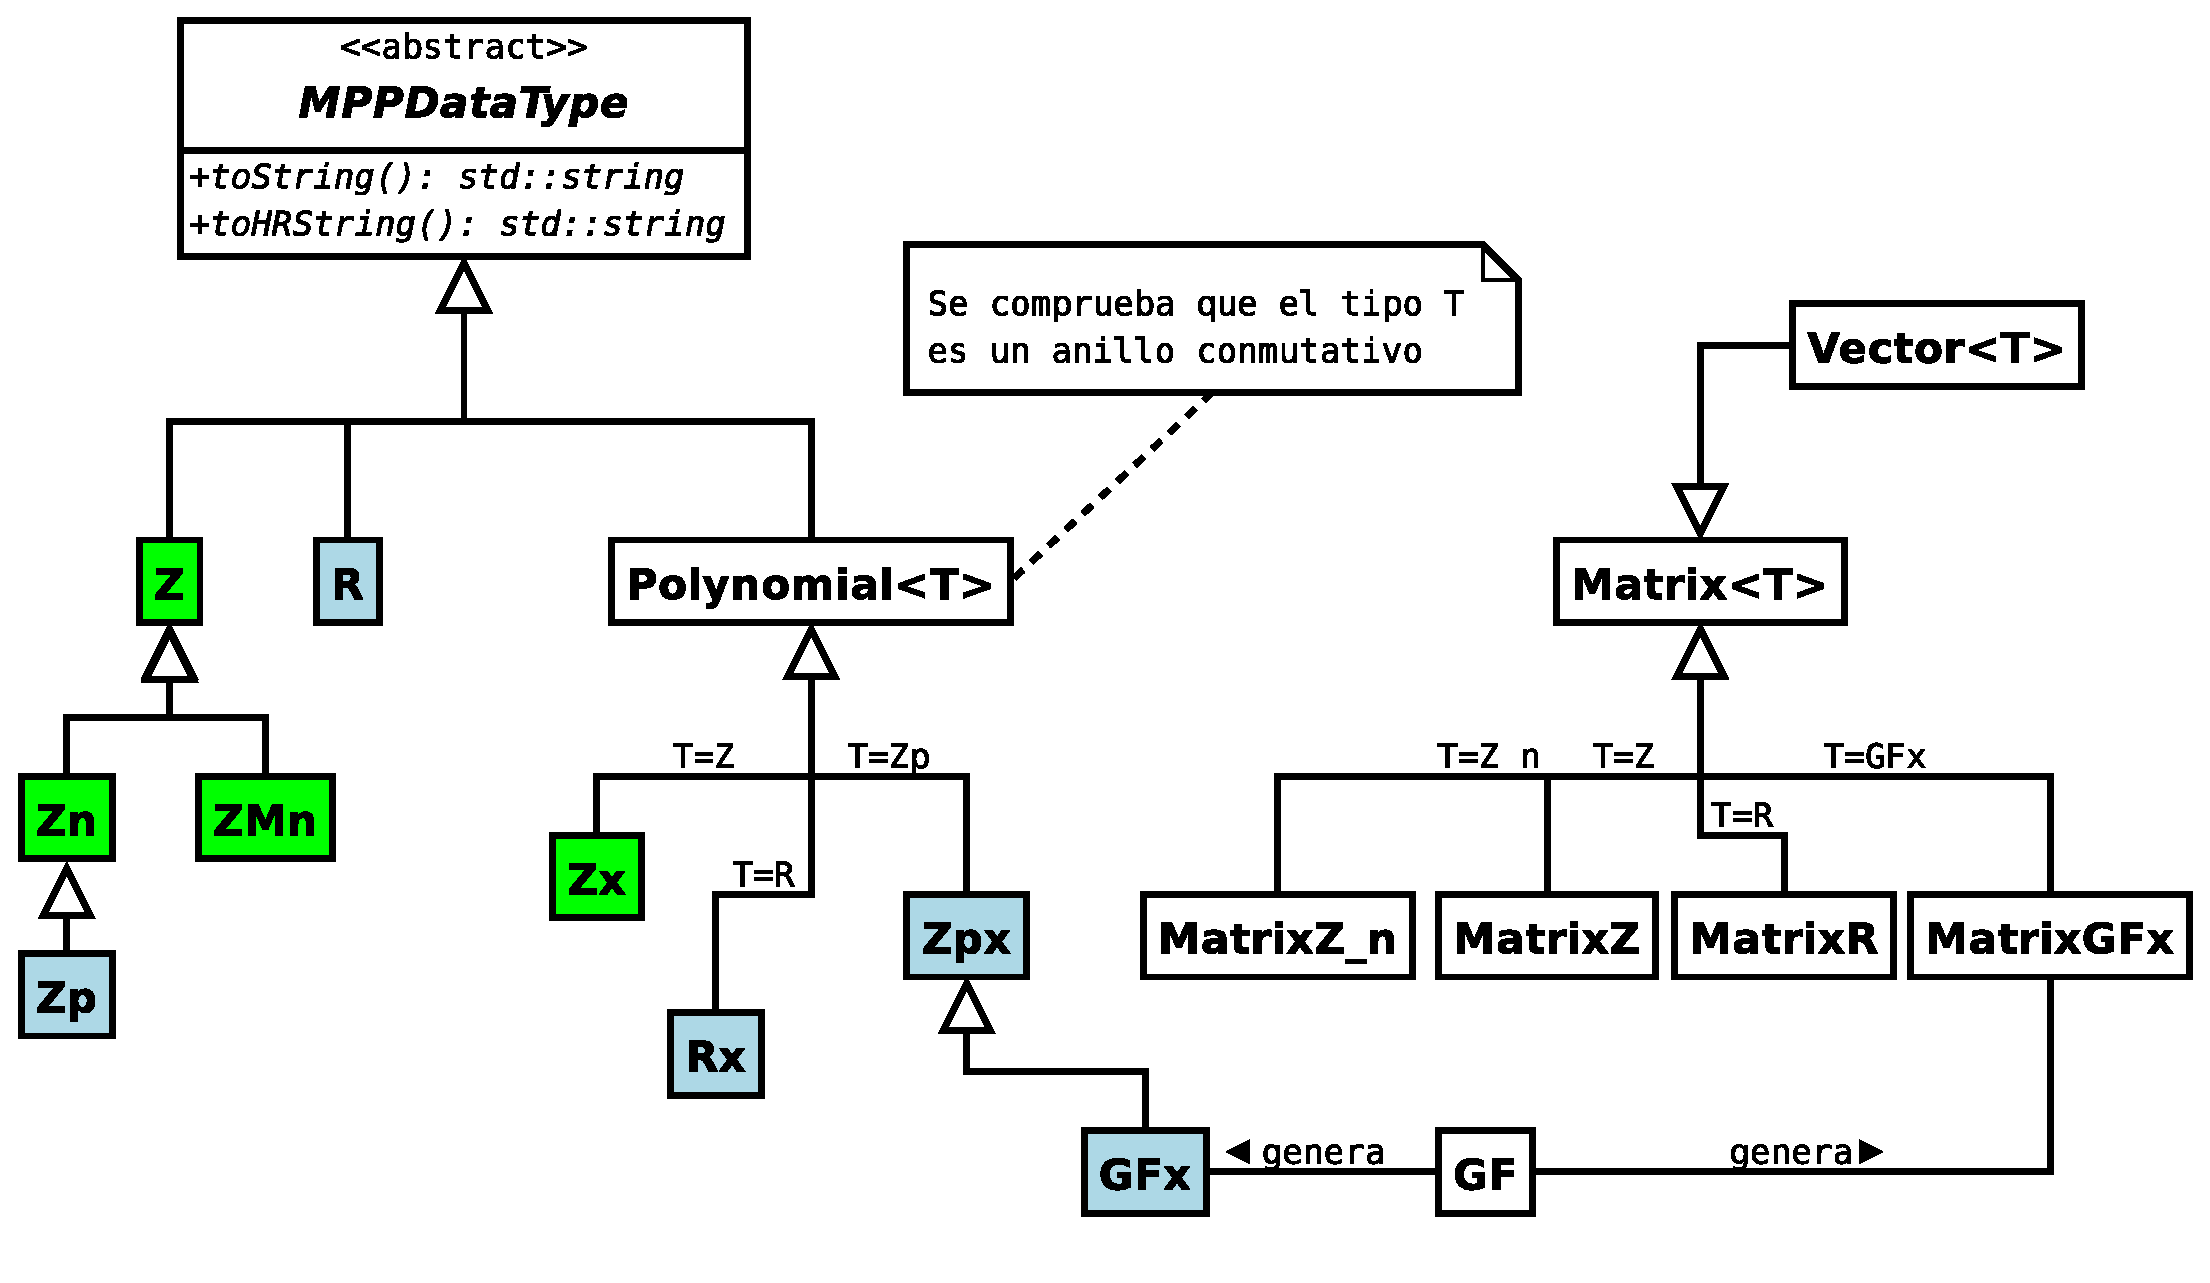
\includegraphics[width=0.95\textwidth,keepaspectratio]{categorizacionAlgebraica} 
    \caption{Categorizaci�n algebraica}\label{fig:categorizacionAlgebraica}
  \end{figure}




  \subsection{Enteros $\mathbb{Z}M_n$}\label{implZM_n}

  \subsection{Polinomios}\index{implementaci�n!polinomios}\label{impl:polinomios}
    totalmente genericos
  \subsubsection{Verificando el car�cter de $S$}
    tiene que ser como ser como minimo anillo conmutativo con unidad. Verificaciones estaticas
  \subsubsection{Operaciones dependientes de $S$}
    p ej, div en udf o  no, idem pa gcd  


  \subsection{Matrices}\index{tipos!Matrices}

%% CAPITULO SOBRE LOS N�MEROS PRIMOS

\chapter{N�meros primos}\label{cap:primos}\index{n�meros!primos}

\begin{flushright}
  \begin{minipage}[t]{13cm}
    \begin{flushright}
      \begin{quote}
        \emph{
        \ldots there is no apparent reason why one number is prime and another not.
        To the contrary, upon looking at these numbers one has the feeling of
        being in the presence of one of the inexplicable secrets of creation.
        }
        \begin{flushright}
          \textbf{\textemdash D. Zagier}
        \end{flushright}
      \end{quote}
    \end{flushright}
  \end{minipage}
\end{flushright}

\bigskip

\begin{flushright}
  \begin{minipage}[t]{13cm}
    \begin{flushright}
      \begin{quote}
        \emph{
        So if you could be the Devil and offer a mathematician to sell his soul
        for the proof of one theorem - what theorem would most mathematicians
        ask for? I think it would be the Riemann Hypothesis.
        }
        \begin{flushright}
          \textbf{\textemdash H. Montgomery}
        \end{flushright}
      \end{quote}
    \end{flushright}
  \end{minipage}
\end{flushright}

\bigskip

\begin{center}{\line(1,0){325}}\end{center}

%--------------------------------------------------------%

\section{Introducci�n}
Los n�meros primos juegan un papel important�simo en criptograf�a.
Por ejemplo, v�ase el papel que juegan en el problema FACTORING
(secci�n \ref{factoring}) y por ende en muchos de los dem�s problemas
de la secci�n \ref{problemasFundamentales} que se reducen a �ste. No
es menos importante su presencia en la Teor�a de N�meros.

En esta secci�n se presentan los mecanismos que la librer�a ofrece
para el trabajo con primos.


\section{Resultados importantes}
Se recogen aqu� algunos resultados que ser�n citados a lo largo de
este cap�tulo.

\subsection{El teorema de los n�meros primos}
Uno de los grandes hallazgos de la Teor�a de N�meros del siglo XIX,
demostrado de forma independiente por Hadamard y Poussin en 1896
(\cite{countingPrimes}). Su formulaci�n original es:

  \begin{teorema}[Teorema de los n�meros primos]\label{teoremaPrimos}
      El n�mero de primos menores o iguales que $x$ es asint�ticamente igual a
      $\frac{x}{\ln{x}}$.
  \end{teorema}

  El concepto de ``n�mero de primos menores o iguales que $x$'' cuenta con su
  propia funci�n, y nada menos que representada por la letra griega
  posiblemente m�s famosa: $\pi$. Suele denominarse a esta funci�n
  como de \index{primos!recuento}{\emph{recuento de primos}}\label{funcionPi}.
  Mucho se ha escrito acerca de esta funci�n, por ejemplo v�ase
  \cite{riesel}\footnote{p�g. 44 y siguientes}. 

  Una formulaci�n m�s rigurosa de $\pi(x)$ ser�a:
  \[
    \pi(x) = \textrm{Li} + O(x \cdot e^{-a\sqrt{\log(x)})}
  \] 
  con $a$ una constante positiva y
  \[
    \textrm{Li} = \int_{2}^{x} \frac{dt}{\log(t)}
  \]
  denominada la \emph{integral logar�tmica}.

  La Hip�tesis de Riemann citada al comienzo del cap�tulo hace su
  aparici�n aqu�, por tanto que el error de la $\pi(x)$ anterior puede
  reducirse a $O(\sqrt{x} \log(x))$ si �sta es cierta, resultando por
  tanto $\textrm{Li}$ una muy buena aproximaci�n a $\pi(x)$.

  \subsection{Teorema de Mertens}
  Importante resultado a la hora de realizar estimaciones en las
  cribas.

  \begin{teorema}[Teorema de Mertens]\label{mertens}
  Siendo $\gamma$ la constante de Euler-Mascheroni\footnote{
  $\gamma = \lim_{n \rightarrow \infty} \left(\sum_{k=1}^n \frac{1}{k}
  - \ln n \right) \approx 0.57721566490153286060\cdots$},
  \[
   \prod_{2\leq p \leq x} \left( 1 - \frac{1}{p} \right) \sim
   \frac{e^{-\gamma}}{\ln x} = \frac{0.5615}{\ln x}, \qquad
   x\rightarrow \infty
  \]
  \end{teorema}
  
  

\section{Tests de composici�n}\label{testsDeComposicion}
  Los as� denominados son los tests que, cuando se les presenta un 
  n�mero, determinan con un cierto grado de probabilidad la primalidad
    del mismo. Si el n�mero es primo, siempre responden 
    correctamente. Si por contra es compuesto, se
    devuelve la respuesta correcta con probabilidad
    $p$, valor que puede hacerse tan cercano a $1$ como se
    desee, pero sin llegar a serlo. 
    
\subsection{Test de Fermat}
  El test de composici�n m�s simple se basa en el siguiente conocido
  teorema debido a Pierre de Fermat, quien en el siglo XVII fue hombre
  de leyes, dedic�ndose a las matem�ticas a modo de ``afici�n'' (y
  tal y como a Gauss se le llam� el ``principe de los matem�ticos'', a
  Fermat se le ha llegado a llamar el ``principe de los
  aficionados''). Parece que tambi�n ten�a afici�n a plantear
  conjeturas de una considerable longevidad cuyas ``maravillosas
  pruebas'' no cab�an en los m�rgenes.
  \begin{teorema}[Peque�o teorema de Fermat]
  Dado $p$ un primo y $a \in \mathbb{N}$, 
  \[
    a^p \equiv a \pmod{p}
  \]
  Si adem�s $p$ y $a$ son coprimos, entonces 
  \begin{eqnarray*}
    a^p - a & \equiv & 0 \pmod{p} \\
    a(a^{p-1} - 1) & \equiv & 0 \pmod{p} \\
    a^{p-1} & \equiv & 1 \pmod{p} 
  \end{eqnarray*}
  \end{teorema}
  
  As� que d�ndole la vuelta, se tiene que si $a^{n-1} \not\equiv 1 \pmod{n}$
  para $a$ y $n$ coprimos, $n$ \emph{no} puede ser primo, siendo por
  tanto compuesto. Es a esto a lo que se denomina el
  \index{test!Fermat}{\emph{test de Fermat}}.
  
    \subsubsection{Pseudoprimos}
    Por desgracia, esto es una condici�n necesaria pero \emph{no
    suficiente} para demostrar la primalidad de $n$. El n�mero
    \emph{compuesto} que para un determinado $a$ satisface la
    congruencia del test de Fermat se dice
    \index{pseudoprimo}{\emph{pseudoprimo}} para la base $a$.
    Existen incluso pseudoprimos para \emph{todas} las posibles bases $a$, 
    denomin�ndose estos \index{n�meros!de Carmichael}{\emph{n�meros de
    Carmichael}} (por ejemplo, el $561$). Estos n�meros presentan
    propiedades muy interesantes, siendo muy extensa la bibliograf�a al
    respecto. Consultar por ejemplo \cite{riesel}\footnote{p�g. 95}.
    Importante rese�ar que en 1994 Alford, Granville, y Pomerance demuestran la existencia
    de infinitos de estos n�meros de Carmichael.

    La conclusi�n que se saca es que aunque el test de Fermat pueda ser
    �til en algunas ocasiones, no es viable su utilizaci�n en general.
    

  \subsection{El criterio de Euler}\label{criterioEuler}
  Con el siguiente teorema debido a Leonhard Euler\footnote{Marquis de
  Condorcet dir�a de �l a su muerte: ``Euler ces� de vivir y de
  calcular'', ya que sol�a decirse que ``Euler calculaba en apariencia
  sin ning�n esfuerzo, igual que los hombres respiran o que las
  �guilas se sostienen en el aire''}
  se presenta un panorama mejor:
  \begin{teorema}[Criterio de Euler]\label{tma:criterioEuler}
  Sean $a \in \mathbb{N}$ y $p > 2$ primo coprimos. Entonces
  \[ 
    \left( \frac{a}{p} \right) \equiv a^{(p-1)/2} \pmod{p}
  \]
  ($\left( \frac{a}{p} \right)$ representa el s�mbolo de Legendre, v�ase 
  \ref{simboloLegendre})
  \end{teorema}
  Entonces, para $a$ y $n > 2$ coprimos siendo $n$ primo, se cumple
  $a^{(n-1)/2} \equiv \pm{1} \pmod{n}$.
  Como para el caso anterior, si a esto se le da la vuelta, se tiene
  que si $a^{(n-1)/2} \not\equiv \pm{1} \pmod{n}$, $n$ \emph{no} puede 
  ser primo y ser� por tanto compuesto. Y a�n as�, aunque la
  equivalencia se cumpliera, restar�a comparar el valor de $a^{(n-1)/2}$ 
  con el del s�mbolo de Jacobi $\left(
  \frac{a}{n} \right)$. Si ambos difieren m�dulo $n$, $n$ ser�
  compuesto. Si coinciden, no es posible concluir nada, ya que esto
  precisamente es el \index{QRP}{QRP} (v�ase \ref{qrp}).

  Hasta ahora, tenemos fundamentalmente lo mismo que se ten�a con el
  test de Fermat: una condici�n necesaria pero \emph{no} suficiente. Y aqu�
  tambi�n hay mentirosos.
  \subsubsection{Pseudoprimos de Euler}\label{pseudoprimosDeEuler}
  \begin{definicion}[Pseudoprimo de
      Euler]\label{def:pseudoprimoDeEuler}
    Si un n�mero compuesto $n$ satisface 
    \[ 
      \left( \frac{a}{n} \right) \equiv a^{(n-1)/2} \pmod{n}
    \]
    para $a$ coprimo con �l, se tiene un \index{pseudoprimo!de
    Euler}{\emph{pseudoprimo de Euler}} para la base $a$.
  \end{definicion}
    Sin embargo, lo interesante viene ahora:
    \begin{teorema}\label{noExitenciaCarmichael}
      No existe un concepto an�logo a los \index{n�meros!de Carmichael}
      {n�meros de Carmichael} para los pseudoprimos de Euler. Esto es, 
      si se prueba con las suficientes bases $a$, se revelar� la
      composici�n (o primalidad) del n�mero a prueba.
    \end{teorema}
    
    \subsection{Pseudoprimos fuertes}\label{pseudoprimosFuertes}
    El teorema \ref{noExitenciaCarmichael} se hace extensivo a otro 
    concepto �ntimamente relacionado:
    \begin{definicion}[Pseudoprimos
      fuertes]\label{def:pseudoprimosFuertes}
      Un n�mero compuesto $n$ con $n-1 = d \times 2^s$ tal que $d$
      impar, se denomina \index{pseudoprimo!fuerte}{\emph{pseudoprimo
      fuerte}} para la base $a$ si
      \[
        a^d \equiv 1 \pmod{n} 
      \]
      o bien
      \[
        a^{d\times2^r} \equiv -1 \pmod{n} 
      \]
      para alg�n $r \in [0,1,\cdots, s-1]$.
    \end{definicion}
    Este concepto es �til ya que se demuestra que es una condici�n m�s
    restrictiva que las impuestas por el criterio de Euler. De hecho,
    engloba los conceptos del test de Fermat, del criterio de Euler y
    de los n�meros de Carmichael ---en el sentido ya expuesto de no
    tener algo an�logo---; una base $a$ para la que $n$ es un
    pseudoprimo fuerte, tambi�n lo es bajo el criterio de Euler. A su
    vez, si $a$ es base de un pseudoprimo de Euler $n$, tambi�n lo ser� en
    el test de Fermat (\cite{handbook}\footnote{p�g. 140, punto
    4.30}).
    

  \subsection{Test de Rabin-Miller}\label{testRabinMiller}
  El test de composici�n m�s utilizado dada su facilidad de
  implementaci�n y su potencia. Virtualmente todo paquete que
  permita comprobar el car�cter primo de un n�mero, desde el tit�n 
  Mathematica hasta la m�s modesta librer�a para el trabajo con Teor�a
  de N�meros, incluye este m�todo en alg�n punto.
  Para justificar su validez se necesitan dos resultados previos:

  \begin{teorema}
    Para $n \in \mathbb{Z}$ compuesto, como m�ximo $\frac{1}{4}$ de
    los n�meros menores que $n$ son bases para las que el test de
    pseudoprimo fuerte se satisface, arroj�ndose un falso positivo. 
    (\cite{handbook}\footnote{p�g. 139. Punto 4.23})
  \end{teorema}
  \begin{teorema} 
    Sean $x$, $y$, $n$ enteros. Si $x^2 \equiv y^2 \pmod{n}$ pero 
    $x \not\equiv \pm{y} \pmod{n}$, entonces el m�ximo com�n divisor
    de $(x-y)$ y $n$ ser� un divisor no trivial de $n$.
    (\cite{handbook}\footnote{p�g. 94. Punto 3.18})
  \end{teorema}
  
  La formulaci�n b�sica de este algoritmo se muestra por ejemplo en
  \cite{schneier}\footnote{p�g. 260}. Sin embargo, en la pr�ctica hay
  varios aspectos a considerar para conseguir resultados en un menor
  tiempo. El primero es el realizar una comprobaci�n de divisibilidad
  entre los primos menores a una determinada cota. En
  \cite{schneier} se discute el valor de esta cota y se da como �ptimo
  el valor $2000$. Ya que $\pi(2000) = 303$, se ha de almacenar una
  tabla con esos $303$ primos menores que $2000$. En la librer�a, esta
  tabla se encuentra bajo el nombre \texttt{Constantes::TABLA\_PRIMOS\_2000}.
  Es m�s, la proporci�n de enteros impares no eliminados por este
  proceso de cribado es: 
  \[
    \prod_{3 \leq p \leq B}{(1-\frac{1}{p})} 
  \]
  que por el Teorema de Mertens (\ref{mertens}),
  es aproximadamente igual a: 
  \[
    \frac{1.12}{\ln{B}} = \frac{1.123}{\ln{2000}} \approx 0.1474
  \]
  (n�tese que $1.123 = 2\times 0.5615$, ya que se consideran s�lo los
  impares)
  con lo que m�s del $85\%$ de los impares a probar se eliminar�n en
  este proceso de criba.
  Estas comprobaciones de divisibilidad se han realizado
  mediante la aplicaci�n de la funci�n del m�ximo com�n divisor.
  Est� claro que para todo $n \leq 2000^2$ esto constituye una
  \emph{prueba de primalidad}; la respuesta dada determina con
  \emph{toda seguridad} el car�cter de $n$.

  La segunda estrategia consiste en aprovechar el conocimiento del
  menor n�mero compuesto que pasa el test de Rabin-Miller para las $k$
  primeras bases primas para concluir de nuevo con \emph{total seguridad} el
  car�cter del n�mero. Es decir, si se sabe que el
  menor n�mero compuesto que pasa el test para las $k$ primeras bases primas es $x$,
  para todo $y < x$ se podr� dar una respuesta \emph{segura} acerca de
  su primalidad sin m�s que ejecutar el test con como m�ximo dichas $k$ bases. 
  Por desgracia, esta t�cnica s�lo vale a d�a de hoy (primera mitad de
  2004) para n�meros menores que $3.4 \times 10^{14}$, ya que esta
  secuencia, referenciada en \cite{sloane} como la A014233, s�lo se
  ha desarrollado hasta el valor $341550071728321$, por Jaeschke en 1993. La
  secuencia en cuesti�n es:
  \begin{eqnarray*}
    \psi_1 & = & 2047 \\
    \psi_2 & = & 1373653 \\
    \psi_3 & = & 25326001 \\
    \psi_4 & = & 3215031751 \\
    \psi_5 & = & 2152302898747 \\
    \psi_6 & = & 3474749660383 \\ 
    \psi_7 & = & 341550071728321 \\
    \psi_8 & = & 341550071728321 
  \end{eqnarray*}
  siendo el sub�ndice de $\psi$ el citado $k$. El valor para $k=8$ no
  es una errata, efectivamente no aporta nada, por lo cual en la
  implementaci�n se considerar� como m�ximo $k=7$.
  
  La tercera y �ltima cuesti�n a considerar es que, seg�n
  \cite{handbook}\footnote{p�g. 140, punto 4.28}, el producto 
  de dos bases que satisfacen la definici�n \ref{def:pseudoprimosFuertes}
  de \index{pseudoprimo!fuerte}{pseudoprimo fuerte}
  es, muy posiblemente, tambi�n una base que produce un pseudoprimo fuerte,
  as� que parece razonable utilizar como bases primos sucesivos, lo
  cual facilita adem�s la implementaci�n de la estrategia anterior, ya que
  el probar bases primas ser� la norma general.

  Teniendo todo esto en consideraci�n, la formulaci�n queda de la
  manera expuesta en el algoritmo \ref{alg:rabinMiller}. La
  complejidad computacional de este algoritmo es fundamentalmente
  ---obviamente las variables ocultas ser�n mayores--- la del algoritmo de
  potenciaci�n modular utilizado.
  \begin{algorithm}
    \caption{Test de Rabin-Miller modificado (Parte 1 de 2)}\label{alg:rabinMiller}
    \begin{algorithmic}[1]
      \Procedure{RabinMillerModificado}{entero $n$, iteraciones $k$}
        \State $n \gets |n|$
        \If{$(n = 1) \vee (n \equiv 0 \pmod{2}) $}
          \State \textbf{devolver} ``Compuesto''
        \EndIf
        \If{$n \leq B^2$}
          \State $cota \gets \lfloor\sqrt{n}\rfloor$
          \State $i \gets 2$
          \While{$i \leq cota$}
            \If{$\gcd(i,n) \neq 1$}
              \State \textbf{devolver} ``Compuesto'' 
            \EndIf
            \State $i \gets siguientePrimo(i)$ 
          \EndWhile
          \State \textbf{devolver} ``Primo'' 
            \Comment{Con total certeza}
        \Else
          \State $cota \gets \pi(B)$ 
            \Comment{$\pi$ representa la funci�n de recuento de primos
            (v�ase \ref{funcionPi})}.
          \State $i \gets 2$
          \While{$i \leq cota$}
            \If{$\gcd(i,n) \neq 1$}
              \State \textbf{devolver} ``Compuesto'' 
            \EndIf
            \State $i \gets siguientePrimo(i)$ 
          \EndWhile

          \State \Comment{Optimizar si es posible el n�mero de
          iteraciones por medio de la secuencia de Sloane.}
          \If{$n < \psi_7$}
           \If{$n < \psi_6$}
            \If{$n < \psi_5$}
             \If{$n < \psi_4$}
              \If{$n < \psi_3$}
               \State $k = 3$ \EndIf
              \Else $k = 4$ \EndIf
             \Else $k = 5$ \EndIf
            \Else $k = 6$ \EndIf
           \Else $k = 7$ \EndIf
        
           \State \Comment{Aqu� ya s� empieza el m�todo ``cl�sico'' de
           Rabin-Miller, con la salvedad de que se consideran las
           bases como los primos sucesivos, en vez de ser n�meros
           aleatorios. V�ase esto en la segunda parte del algoritmo.}
           \EndIf
           \EndProcedure
         \end{algorithmic}
       \end{algorithm}

       \begin{algorithm}
         \caption{Test de Rabin-Miller modificado (Parte 2 de 2)}\label{alg:rabinMiller2}
         \begin{algorithmic}[1]
           \State Determinar $r$ y $s$ tales que $n-1 = 2^s \times r$
           \State $a \gets 1$
           \For{$i=0$ hasta $i=k$}
            \State $a \gets siguientePrimo(a)$
            \State $y = a^r \bmod n$\label{subAlg:RM1}
            \If{$(y \neq 1) \wedge (y \neq n-1)$}
              \State $j \gets 1$
              \While{$(j \leq s-1) \wedge (y \neq n-1)$}
                \State $y \gets y^2 \bmod n$\label{subAlg:RM2}
                \If{$y = 1$}
                  \State \textbf{devolver} ``Compuesto'' 
                \EndIf
                \State $j \gets j+1$
              \EndWhile
              \If{$y \neq n-1$}
                \State \textbf{devolver} ``Compuesto'' 
              \EndIf
            \EndIf
           \EndFor
           \State \textbf{devolver} ``Primo'' 
    \end{algorithmic}
  \end{algorithm}

  
  En relaci�n con la segunda cita incluida al comienzo del cap�tulo, 
  se�alar que como indica \cite{riesel}\footnote{p�g. 99}, Gary Miller
  (como es f�cil de adivinar, parte importante del desarrollo del
  m�todo Rabin-Miller) demostr� que, \emph{asumiendo como cierta la Hip�tesis
  de Riemann Generalizada}, los tests que se apoyan en el concepto de
  pseudoprimo fuerte, tal como es el para su m�todo cuasi-hom�nimo,
  pueden constituir un test de \emph{primalidad} en tiempo polinomial.
  Y es seguro que no queda claro el enorme papel que la c�lebre
  Hip�tesis de Riemann juega en la Teor�a de N�meros con s�lo lo
  expuesto en la presente memoria, pero
  ciertamente es uno de los conceptos recurrentes en muchas de las ramas 
  de la Matem�tica. 
  Es muy amena e interesante la lectura de \cite{constants} para tener
  una peque�a visi�n de todo esto. 

  \subsection{Otros tests}
  Existen otros tests de composici�n probabil�sticos como el de
  Rabin-Miller, siendo quiz�s uno de los m�s conocidos el de 
  Slovay-Strassen. Este m�todo es una aplicaci�n directa del concepto
  de \index{pseudoprimo!de Euler}{pseudoprimo de Euler} y del teorema
  \ref{tma:criterioEuler}, como se ve en el algoritmo
  \ref{alg:slovayStrassen}.

  \begin{algorithm}
    \caption{Test de Slovay-Strassen}\label{alg:slovayStrassen}
    \begin{algorithmic}[1]
      \Procedure{SlovayStrassen}{entero $n$, iteraciones $k$}
      \For{$i=0$ hasta $i=k$}
        \State $a \gets r \in (1,n-1) aleatorio$
        \State $r \gets a^{(n-1)/2} \bmod n$
        \If{$(r \neq 1) \wedge (r \neq n-1)$}
          \State \textbf{devolver} ``Compuesto''
        \EndIf
        \State $s \gets \left( \frac{a}{n} \right)$ 
          \Comment{S�mbolo de Jacobi}
          \If{$r \not\equiv s \pmod{n}$}
            \State \textbf{devolver} ``Compuesto''
        \EndIf
      \EndFor
      \State \textbf{devolver} ``Primo''
      \EndProcedure
    \end{algorithmic}
  \end{algorithm}

  La elecci�n del m�todo de Rabin-Miller como el incluido de serie en
  la librer�a sobre el m�todo de Slovay-Strassen no ha sido
  caprichosa. Se apoya en estos puntos:
  \begin{enumerate}
    \item Es m�s costoso, b�sicamente a causa de calcular para cada
      iteraci�n un s�mbolo de Jacobi $\left( \frac{a}{n} \right)$ para
      un $n$ potencialmente muy grande, teniendo en cuenta que esta
      operaci�n tiene un coste $O(\log^2{n})$. %todo: completar
    \item El error del m�todo Slovay-Strassen est� acotado por
      $\left(\frac{1}{2}\right)^k$ con $k$ el n�mero de iteraciones,
      mientras que para Rabin-Miller esta cota es de $\left(\frac{1}{4}\right)^k$.
    \item Por lo dicho en \ref{pseudoprimosFuertes}, Rabin-Miller
      nunca ser� ``peor'' que Slovay-Strassen, al apoyarse en el
      concepto de pseudoprimo fuerte, frente al de pseudoprimo de Euler
      del m�todo de Slovay-Strassen.
  \end{enumerate}
\section{Tests de primalidad}\label{testsDePrimalidad}
  Frente a los tests de composici�n (v�ase \ref{testsDeComposicion}),
  los tests de primalidad dan una respuesta totalmente certera sobre
  el car�cter primo de un n�mero\footnote{Algunos autores como
  \cite{riesel,cohen} hablan de \emph{demostraci�n} de la primalidad.
  Aunque ciertamente puede verse as�, hay quien discrepa ---de forma
  un tanto rom�ntica--- sobre si esto constituye una demostraci�n en
  el sentido ``cl�sico''. El denominado ``problema de los cuatro
  colores'' es el caso cl�sico de demostraci�n mediante el uso de
  ordenadores. Una muy amena lectura divulgativa sobre esto es
  \cite{fermat}, p�g. 280 y siguientes.}.
  
  Entonces, �por qu� no se han implementado
    tests de \index{test!primalidad}{\emph{primalidad}}? Estos dan con
    una total certeza una respuesta a la pregunta acerca de la
    primalidad (que no composici�n simplemente) de un n�mero 
    (v�ase \ref{testsDePrimalidad}), �as�
    pues? Pues bien, las razones fundamentalmente han sido dos:
    \begin{enumerate}
      \item El coste computacional es notablemente superior. El mejor
        algoritmo en este sentido del que se tiene conocimiento a la
        hora de escribir esto (primera mitad de 2004) es el denominado
        AKS, del cual en \cite{AKS} se dice est� en $O(\log^{10.5}
        {n})$, con la posibilidad de bajar esta cota de cumplirse
        ciertas conjeturas\footnote{\textit{Ib�dem, pp. 6,7}}. A�n as�,
        las constantes ocultas son muy considerables, lejos del
        $O(\log^{2}{n})$ del m�todo de Rabin-Miller, adem�s de ser un
        algoritmo considerablemente m�s complejo de implementar.
      \item No existe una necesidad \emph{real} de estos m�todos. A�n
        cuando un test de composici�n se ejecute con una probabilidad de
        error equivalente a la de ganar la loter�a estatal de Estados
        Unidos y ser fulminado por un rayo el mismo d�a (probabilidad $1/2^{55}$
        seg�n \cite{schneier}\footnote{p�g. 18}), tan s�lo supondr�an
        $27$ iteraciones en el m�todo de Rabin-Miller (v�ase
        \ref{testRabinMiller}), y esto siendo extremadamente
        conservador y pesimista con las estimaciones. 
    \end{enumerate}


 \section{Factorizaci�n}\label{factorizacion}
  La factorizaci�n de enteros es uno de los ``santos griales'' de la
  criptograf�a, por ser precisamente el problema FACTORING expuesto en
  la secci�n \ref{factoring}. 
  Se incluyen en la librer�a una serie de m�todos para la
  factorizaci�n de enteros relativamente ``grandes'', pero desde el
  punto de vista no ya de la criptograf�a, sino m�s bien del usuario: Al
  autor un n�mero de $40$ bits le parece honestamente bastante
  grande; sin embargo nadie en su sano juicio usar�a factores de $40$
  bits en un algoritmo de clave p�blica como RSA para generar un
  entero producto de $80$ bits, el cual podr�a ser roto en
  razonablemente poco tiempo por los sencillos\footnote{\cite{cohen}
  titula al capitulo en el que expone alguno de estos algoritmos como
  ``Factoring in the Dark Ages'', lo cual da una idea de que han sido
  superados ya por otros m�todos.} algoritmos que esta librer�a
  incorpora.

  Cada m�todo tiene un ``espectro'' de acci�n determinado. Es por esto
  que la idea es combinarlos en funci�n de sus particularidades,
  orientando a cada uno a un determinado rango del tama�o del entero a
  factorizar. 

  Por �ltimo, remarcar que la factorizaci�n es un proceso recursivo:
  los algoritmos tratar�n siempre de encontrar un factor no trivial,
  entre el que se dividir� el n�mero a factorizar y vuelta a empezar
  hasta obtener eventualmente un n�mero primo.
  \subsection{Criba}\label{cribaFact}
    Es el m�todo m�s obvio, y consiste en comprobar la divisibilidad
    del n�mero a factorizar $n$ entre todos los primos $\leq
    \sqrt{n}$. 
    En el peor caso, se tendr�a una complejidad de
    aproximadamente $\Omega(\sqrt{n})$ divisiones
    si $n$ est� formado por dos factores
    primos de aproximadamente el mismo tama�o. 
    De media, se tendr�a un n�mero de divisiones en $O(\pi(n))$,
    siendo $\pi$ la funci�n de recuento de primos de la secci�n
    \ref{funcionPi}. En otras palabras, este algoritmo tiene
    complejidad \emph{exponencial}.

    Ahora bien, por el teorema de Mertens (teorema \ref{mertens}), la
    proporci�n de impares que no tienen factores por debajo de una
    cota determinada $B$ se reproduce en la tabla
    \ref{tablaProporFactores}.
    \begin{table}
      \begin{center}\begin{tabular}{|c|c|} 
        \hline 
        \multicolumn{1}{|c|}{$B$}&
        proporci�n\tabularnewline
        \hline
        \hline 
        $10^2$&
        $0.24385$\tabularnewline
        \hline 
        $10^4$&
        $0.121925$\tabularnewline
        \hline 
        $10^6$&
        $0.081282$\tabularnewline
        \hline 
        $10^8$&
        $0.060962$\tabularnewline
        \hline
      \end{tabular}\end{center}
      \caption{Proporci�n de impares sin factores por debajo de $B$}
      \label{tablaProporFactores}
    \end{table}
    Es f�cil ver que esta tabla ha sido construida en base a:
    \[
      \prod_{p \geq 3}^B \left(1-\frac{1}{p}\right) \approx
      2\frac{e^{-\gamma}}{\ln B} = \frac{0.4877}{\log_{10} B}
    \]
    A la vista de estas proporciones, se puede concluir que es
    razonable utilizar un proceso de cribado para tratar de extraer
    los factores peque�os de una forma r�pida. 

    \paragraph{Estimaci�n de la cota.}
    Saber en qu� momento abandonar el proceso de cribado es
    fundamental dado el car�cter exponencial del mismo; si la cota es
    demasiado grande la complejidad del proceso de factorizaci�n se
    dispara. Por otra parte, no ha de ser excesivamente peque�a ya que
    entonces carecer�a de sentido realizar el proceso. Como casi
    siempre, hay que encontrar una soluci�n balanceada.
    Primero, siempre que hay primos de por medio, ha de tenerse presente la
    especial distribuci�n de los mismos, que el teorema
    \ref{teoremaPrimos} muestra: La densidad de primos puede
    aproximarse por la funci�n decreciente $1/\ln x$ como muestra la
    figura \ref{fig:densidadDePrimos}.

    \begin{figure} \label{fig:densidadDePrimos}
    \begin{center}
        %GNUPLOT: LaTeX picture with Postscript
\begin{picture}(0,0)%
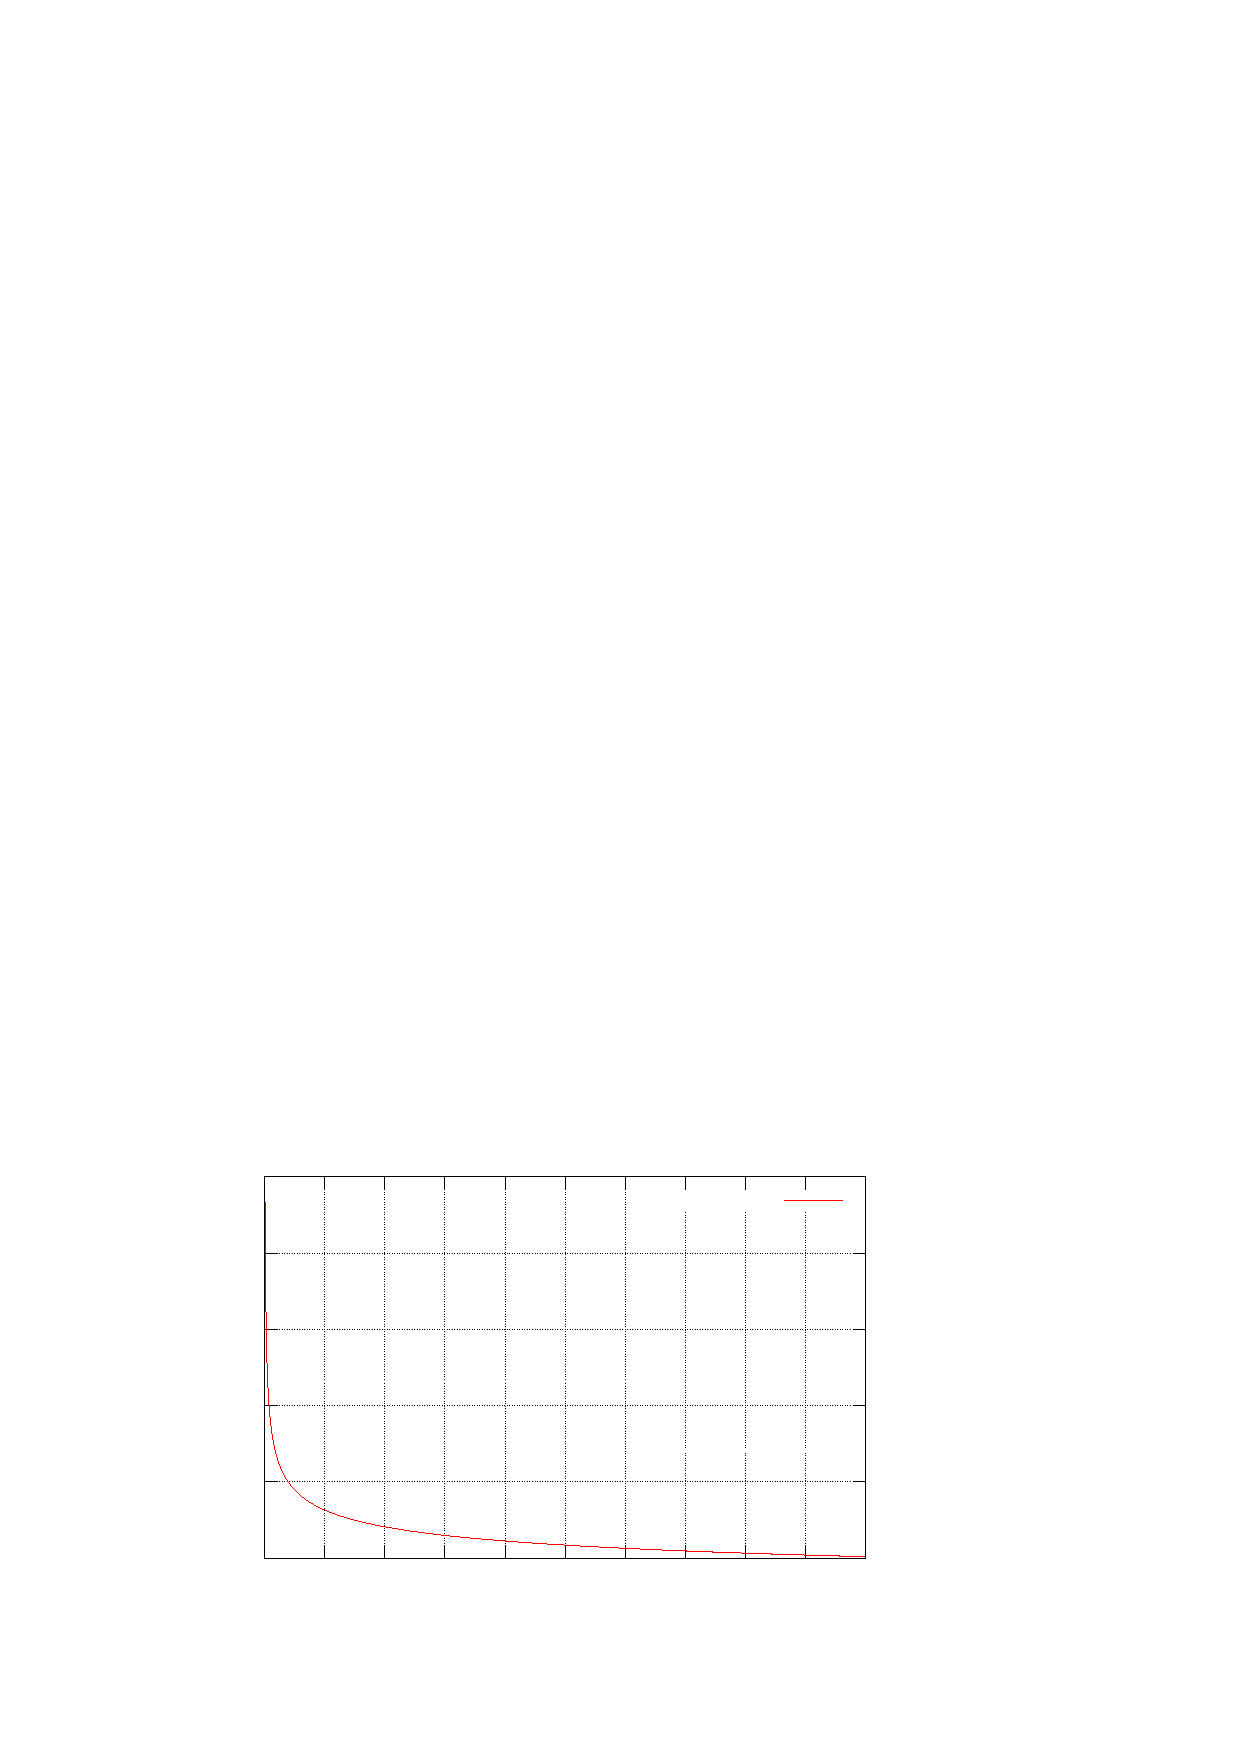
\includegraphics{densidadPrimos}%
\end{picture}%
\begingroup
\setlength{\unitlength}{0.0200bp}%
\begin{picture}(18000,10800)(0,0)%
\put(2475,1100){\makebox(0,0)[r]{\strut{} 0.1}}%
\put(2475,2930){\makebox(0,0)[r]{\strut{} 0.15}}%
\put(2475,4760){\makebox(0,0)[r]{\strut{} 0.2}}%
\put(2475,6590){\makebox(0,0)[r]{\strut{} 0.25}}%
\put(2475,8420){\makebox(0,0)[r]{\strut{} 0.3}}%
\put(2475,10250){\makebox(0,0)[r]{\strut{} 0.35}}%
\put(2750,550){\makebox(0,0){\strut{} 0}}%
\put(4192,550){\makebox(0,0){\strut{} 2000}}%
\put(5635,550){\makebox(0,0){\strut{} 4000}}%
\put(7077,550){\makebox(0,0){\strut{} 6000}}%
\put(8520,550){\makebox(0,0){\strut{} 8000}}%
\put(9962,550){\makebox(0,0){\strut{} 10000}}%
\put(11405,550){\makebox(0,0){\strut{} 12000}}%
\put(12847,550){\makebox(0,0){\strut{} 14000}}%
\put(14290,550){\makebox(0,0){\strut{} 16000}}%
\put(15732,550){\makebox(0,0){\strut{} 18000}}%
\put(17175,550){\makebox(0,0){\strut{} 20000}}%
\put(550,5675){\rotatebox{90}{\makebox(0,0){\strut{}Densidad}}}%
\put(14950,9675){\makebox(0,0)[r]{\strut{}1/log(x)}}%
\end{picture}%
\endgroup
\endinput

    \end{center}
    \caption{Densidad de primos}
  \end{figure}

    El valor $2000$ parece adecuado por varios motivos: por el
    teorema de Mertens (teorema \ref{mertens}) s�lo un poco m�s del
    $7\%$\footnote{$0.5615/\ln{2000} \approx 0.07386$} de los enteros
    no tendr�n factores por debajo de $2000$; ya se dispone de una
    tabla de los $303 = \pi(2000)$ primos menores de $2000$ calculada
    (la cual se utiliza en el tests de Rabin-Miller ---v�ase
    \ref{testRabinMiller}) y a la vista de la gr�fica de la figura
    \ref{fig:densidadDePrimos} parece un buen punto, estando ya
    pr�ximo a la zona en la que la densidad de primos es baja y sigue
    descendiendo a un ritmo lento.
    Por �ltimo, el uso de una cota tan peque�a
    (\cite{cohen}\footnote{p�g. 413} recomienda incluso utilizar
    $500000$ como cota) se justifica por la presencia del m�todo
    $\rho$ de Pollard, que se encarga mucho mejor de los factores
    peque�os que la criba. 

  \subsection{$\rho$ de Pollard}\label{rhoPollard}
  Este m�todo de factorizaci�n est� especialmente indicado para la
  b�squeda de factores peque�os. 
  
  En la siguiente definici�n, se utiliza la misma terminolog�a en
  cuanto a $\lambda$ y $\mu$ que en el teorema
  \ref{existenciaDeCiclos}. Asimismo, se remite al lector a ese
  teorema, relativo a la existencia de ciclos, como paso previo a la
  definici�n que sigue:
  \begin{definicion}[B�squeda de ciclos de Floyd]
    Comenzando con el par $(x_1,x_2)$, calcular sucesivamente pares de
    la forma $(x_i,x_{2i})$ a partir de $(x_{i-1},x_{2i-2})$, hasta
    que $x_m = x_{2m}$ para alg�n $m$. Si la ``cola'' de la secuencia
    tiene longitud $\lambda$ y el ciclo longitud $\mu$, la primera vez
    que se verifique $x_m = x_{2m}$ es cuando $m = \mu(1+\lfloor
    \lambda/\mu \rfloor )$. 
  \end{definicion}

  El meollo del m�todo $\rho$ de Pollard se basa en el siguiente
  razonamiento: \\
  Sea $p$ un factor primo de un compuesto $n$. Se trata de encontrar
  duplicados en la secuencia $x_0,x_1,\cdots$ definida por\footnote{En
  realidad, la secuencia siguiente se define como generada por una
  funci�n aleatoria. Sin tener esto nada que ver con todo lo tratado
  en el cap�tulo \ref{cap:random}\ldots tan solo se pretende que la
  secuencia no sea una procesi�n de valores sucesivos, para facilitar
  la b�squeda de ciclos de la que se hablar� posteriormente. Se
  comprueba que las funciones del tipo $x_{i+1} = f(x_i) = x_i^2 + a$
  funcionan bien, \emph{excepto} para los casos $a=-2$ y $a=0$. Normalmente
  suele utilizarse el valor $a=1$. Sin embargo, n�tese que la elecci�n
  de esta funci�n aleatoria es arbitraria con la salvedad
  de los casos anteriormente citados $a=-2$ y $a=0$.}  
  $x_0 = 2$,
  $x_{i+1} = f(x_i) = x_i^2 + 1 \bmod p$ para $i \geq 0$. Mediante el
  anteriormente citado m�todo de busqueda de ciclos de Floyd, se
  buscar�an dos elementos, $x_m$ y $x_{2m}$, tales que $x_m \equiv x_{2m}
  \pmod{p}$. Pero claro, �$p$ es precisamente lo que estamos buscando! 
  En su lugar, se trabajar� reduciendo m�dulo $n$ en vez de m�dulo
  $p$. As�, en el momento en el que se encuentren valores $x_m$ y
  $x_{2m}$ tales que $1 < d = \gcd(x_m - x_{2m},n) < n$, se habr�
  encontrado un factor no trivial $d$ (posiblemente distinto de $p$,
  pero eso no supone ningun problema). La justificaci�n se deriva de la
  propiedad (\ref{cong6}) de la secci�n \ref{congruencias}, por la que
  se tendr�a $x_m \equiv x_{2m} \pmod{p}$, al ser $p$ divisor de $n$.
  Entonces, al realizar el c�lculo del m�ximo com�n divisor 
  $\gcd(x_m - x_{2m},n)$, casi con total seguridad (existe una
  peque��sima probabilidad de que de este c�lculo salga $n$, lo que no
  aportar�a nada. Si esto ocurre, habr� de utilizarse otra funci�n
  aleatoria $f()$ para la generaci�n de la secuencia $x_i$ si se pretende
  seguir utilizando este m�todo para factorizar $n$) se se obtendr�a un divisor
  no trivial de $n$, ya que
  si $x_m \equiv x_{2m} \pmod{p}$, habr� un alg�n factor de $n$ (el
  propio $p$ o cualquier otro factor no trivial) que saldr� necesariamente a la
  luz con el c�lculo del m�ximo com�n divisor citado.

  Resta, sin embargo, tener alguna certeza de que las colisiones se
  vayan a producir con una frecuencia suficiente como para que este
  m�todo no sea in�til. Pollard demostr� que en una secuencia de
  enteros, reducida m�dulo $p$, un elemento se repite tras tan solo
  $C\sqrt{p}$ pasos, para una constante $C$. Aqu� aparece una idea ya
  presentada en el cap�tulo \ref{cap:fundamentosCriptograficos}: la
  (mal llamada) paradoja del cumplea�os. V�ase \ref{ataqueCumple}.
  Se pueden encontrar tratamientos en profundidad del m�todo de la $\rho$ de
  Pollard en \cite{riesel}\footnote{pp. 174-184},
  \cite{knuth2}\footnote{pp. 369-371, bajo el nombre de
  ``Factorizaci�n � la Monte Carlo''.} y en especial \cite{cohen}\footnote{pp.
  419-425}.

  Este m�todo toma la forma mostrada en el algoritmo
  \ref{alg:rhoPollard}. Como se puede apreciar, uno de los puntos a
  favor de este m�todo es su facilidad de implementaci�n.

   \begin{algorithm}
     \caption{Algoritmo de factorizaci�n $\rho$ de Pollard}\label{alg:rhoPollard}
    \begin{algorithmic}[1]
      \Procedure{RhoPollard}{entero $n$}
      \State $a \gets 2$
      \State $b \gets 2$
      \For{$i=1$ hasta $i=CotaRhoPollard$}
        \State $a \gets a^2+1 \bmod n$
        \State $b \gets b^2+1 \bmod n$
        \State $b \gets b^2+1 \bmod n$ \Comment{No, no es una errata}
        \State $d \gets \gcd(a-b,n)$
        \If{$1 < d < n$}
          \State \textbf{devolver} $d$ como divisor no trivial de $n$.
        \Else
          \If{$d=n$}
            \State \textbf{devolver} Error, necesario cambiar funci�n
            aleatoria.
          \EndIf
        \EndIf
      \EndFor
      \State \textbf{devolver} No se ha encontrado divisor no trivial
      tras $CotaRhoPollard$ iteraciones.
      \EndProcedure
    \end{algorithmic}
  \end{algorithm}



  Ha de se�alarse que este m�todo, en algunas ocasiones, devuelve
  factores no primos. Sin embargo, esto se ataja convenientemente al
  someter al n�mero a factorizar a un proceso de cribado, como se
  describe en la secci�n \ref{cribaFact}, previamente a la ejecuci�n del algoritmo que
  implemente este m�todo de la $\rho$ de Pollard.
  
\section{Generaci�n de primos}
 La generaci�n de n�meros primos es una parte fundamental de la
 criptograf�a de clave p�blica (v�ase \ref{clavePublica}). Que �sta
 sea eficiente es por tanto fundamental.

 El esquema utilizado es bastante sencillo, descansando en los tests
 antes descritos para comprobar si un n�mero impar generado aleatoriamente
 es o no primo. De serlo, hemos terminado. En caso contrario, se
 puede incrementar dicho n�mero en dos unidades (obviamente, para que
 siga siendo impar) o bien volver a generar
 aleatoriamente otro n�mero impar y repetir el proceso.
 Hacer esto es razonable a la vista del teorema \ref{teoremaPrimos},
 por el cual, en su formulaci�n m�s simple (aproximando por
 $(x/\ln{x})$), se tiene que la densidad de primos alrededor de un
 n�mero $n$ ser� de aproximadamente $1/\ln{n}$, con lo que para
 generar un primo de, por ejemplo, $256$ bits en el peor de los casos
 se realizar�n $\ln{2^{256}}$ comprobaciones. Pero dado que s�lo se
 consideran los impares, esta cifra se vuelve la mitad, qued�ndonos
 con una cota superior de $(\ln{2^{256}}/2) \approx 88$ comparaciones.
  \subsection{Estimaci�n del n�mero �ptimo de iteraciones}
    Ahora bien, los tests utilizados son probabil�sticos, y por lo
    tanto, dan su respuesta con un cierto grado de certeza (v�ase
    \ref{testsDeComposicion}). Entonces surge la pregunta �qu� puede 
    considerarse ``certero''?
    Un valor que suele darse por adecuado es la probabilidad de error 
    $\left( \frac{1}{2} \right)^{80}$ ---una probabilidad
    terriblemente peque�a: tal como dice \cite{knuth2}\footnote{p�g.
    379}, y lo dice para $\left( \frac{1}{2} \right)^{50}$, es mucho 
    m�s probable que se produzca el cambio espont�neo del valor de un
    bit debido al mal funcionamiento del hardware 
    que el dar un n�mero compuesto como primo trabajando con esa
    probabilidad de error. Otra forma de verlo es que 
    $\left( \frac{1}{2} \right)^{66}$ es la probabilidad de morir 
    fulminado por un rayo a lo largo de un d�a\ldots \emph{�dos
    veces!}
    
    La estimaci�n de que el test de Rabin-Miller responde con una
    certeza no menor que $\left( \frac{1}{4} \right)^k$ tras $k$
    iteraciones es muy pesimista y conservadora. Para valores
    ``grandes'', es posible reducir considerablemente el n�mero 
    de iteraciones necesario para garantizar la citada 
    probabilidad de $(1/2)^{80}$. En \cite{handbook}\footnote{pp.
    146-148} hay un an�lisis muy interesante de estas cotas de
    probabilidad para diferentes valores del n�mero a probar por el
    m�todo de Rabin-Miller. Concretamente, utilizando los datos de 
    la tabla 4.4 en la p�gina 148 de ese texto se han implementado 
    los m�todos de generaci�n de primos de la librer�a, optimizando
    as� el n�mero de iteraciones (ya que dado que normalmente se
    quiere generar primos grandes ---de entre 256 y 2048 bits)
    necesario, ya que en otros textos como \cite{schneier} simplemente
    se se�ala utilizar siempre cinco iteraciones, mientras que ya a
    partir de $650$ bits no son necesarias tantas para garantizar una
    probabilidad de error menor que $(1/2)^{40}$ (y por otra parte,
    para valores de $500$ y menos bits, son necesarias \emph{m�s} para
    garantizar esa misma cota de probabilidad).
    
    \subsection{\index{primos!fuertes}{Primos fuertes}}\label{primosFuertes}
      Se denominan con este nombre los primos que satisfacen una serie
      de propiedades, a saber (\cite{schneier,handbook}):
      \begin{itemize}
        \item El m�ximo com�n divisor de $(p-1)$ y $(q-1)$ ha de ser
          peque�o.
        \item $(p-1)$ y $(q-1)$ han de tener factores primos grandes
          \footnote{en sentido relativo a los dem�s factores, que habr�n de ser
          considerablemente menores},
          que se denominar�n $p'$ y $q'$.
        \item $(p'-1)$ y $(q'-1)$ han de tener factores primos grandes.
        \item $(p +1)$ y $(q +1)$ han de tener factores primos grandes.
        \item Tanto $\frac{p-1}{2}$ como $\frac{q-1}{2}$ han de ser
          primos.
      \end{itemize}
      Estas propiedades est�n pensadas para que m�todos de
      factorizaci�n como el de la
      $(\rho-1)$ de Pollard pierdan su efectividad. 
      Sin embargo, con la aparici�n de m�todos de factorizaci�n
      basados en t�cnicas de reciente desarrollo como el m�todo de
      curva el�ptica ---ECM, de sus siglas en ingl�s. V�ase
      \cite{cohen}\footnote{pp. 476-481}--- y la criba
      cuadr�tica multipolinomial ---MPQS, de sus siglas en ingl�s. V�ase
      \cite{cohen}\footnote{pp. 482-486}--- hace
      que el uso de estos primos carezca pr�cticamente de sentido. Es
      m�s, \cite{schneier} recomienda \emph{no} utilizarlos:
      \begin{quotation}
        I recommend against specifically generating strong primes. The
        length of the primes is much more important than the
        structure. Moreover, structure may be damaging because it is
        less random.
      \end{quotation}

      La generaci�n de primos fuertes tiene el mismo orden de
      complejidad que el test de Rabin-Miller. Obviamente las
      constantes ocultas ser�n mayores. El algoritmo
      \ref{alg:primosFuertesGordon} muestra la implementaci�n elegida, 
      tambi�n denominado el \index{algoritmo!de Gordon}{algoritmo de
      Gordon (\cite{handbook}\footnote{p�g. 150})}.

      \begin{algorithm}
        \caption{Algoritmo de Gordon para la generaci�n de primos
        fuertes}\label{alg:primosFuertesGordon}
        \begin{algorithmic}[1]
          \Procedure{PFGordon}{tama�o $b$}
          \State $s \gets \textrm{primo aleatorio de } (b/2) \textrm{ bits}$
          \State $t \gets \textrm{primo aleatorio de } (b/2)-2 \textrm{ bits}$
          \State $r \gets (t \times 4)+1$
          \State $t \gets t \times 2$

          \While{ $r$ no es primo }
            \State $r \gets r + t$ 
          \EndWhile
      
          \State $p_0 \gets 2(s^{r-2} \bmod r)s - 1$

          \State $dosRS \gets 2(r \times s)$
          \State $p \gets (p_0 + dosRS)$
          \While{ $p$ no es primo }
            \State $p \gets p + dosRS$ 
          \EndWhile
   
          \State \textbf{devolver} $p$
          \EndProcedure
        \end{algorithmic}
      \end{algorithm}



%% CAPITULO SOBRE GENERADORES RANDOM

\chapter{N�meros
aleatorios}\label{cap:random}\index{n�meros!aleatorios}

\begin{flushright}
  \begin{minipage}[t]{13cm}
    \begin{flushright}
      \begin{quote}
        \emph{
        If your algorithms are great but your random-number generator
        stinks, any smart cryptanalyst is going to attack your system
        through the random-number generation.
        }
        \begin{flushright}
          \textbf{\textemdash Bruce Schneier, ``Applied Cryptography''}
        \end{flushright}
      \end{quote}
    \end{flushright}
  \end{minipage}
\end{flushright}

\bigskip

\begin{flushright}
  \begin{minipage}[t]{13cm}
    \begin{flushright}
      \begin{quote}
        \emph{
        Anyone who considers arithmetical methods of producing random
        digits is, of course, in a state of sin.
        }
        \begin{flushright}
          \textbf{\textemdash John Von Neumann}
        \end{flushright}
      \end{quote}
    \end{flushright}
  \end{minipage}
\end{flushright}

\bigskip

\begin{center}{\line(1,0){325}}\end{center}

%--------------------------------------------------------%

\section{Introducci�n}
La generaci�n de n�meros aleatorios juega un papel fundamental en
numerosos campos, desde la simulaci�n hasta el entretenimiento, pasando
por t�cnicas de muestreo e incluso en an�lisis num�rico (\cite{knuth2}
p�g. 1). 

Se exponen en \cite{brentrandom} nueve casos concretos y de gran
importancia, relativos al uso de n�meros aleatorios en el �mbito de la
computaci�n (y se citan en su d�cimo punto a�n otros doce campos de
aplicaci�n que dicho art�culo no cubre, entre los cuales se encuentra
la criptograf�a). 
La verdad es que merece la pena valerse de uno de esos ejemplos, el
primero, y plasmarlo aqu� y ahora por su belleza, simplicidad y
originalidad: \\
�C�mo comprobar la integridad de la memoria de una sonda espacial\footnote{
En el art�culo (1994) se habla de la sonda Galileo, una misi�n a
J�piter. Dicha sonda finaliz� ya su misi�n el 21 de Septiembre de 2003
desintegr�ndose en la atm�sfera de este planeta.}
que est� a millones de kil�metros de nosotros? La transferencia
completa de la memoria es inviable. Un m�todo que se vale de la
generaci�n de un n�mero primo aleatorio $p$ en un cierto intervalo,
por ejemplo $(10^9, 2 \cdot 10^9)$. Se env�a dicho $p$ aleatorio, de
como m�ximo $\lceil\log_2{(2 \cdot 10^9)}\rceil = 31$ bits y se pide que
la sonda calcule el resto de dividir su memoria, considerada esta como
un entero grande, entre $p$, resultando un n�mero $r_1 < p$ y por
tanto de asimismo $31$ bits a lo sumo. Se han transmitido pues como
m�ximo $62$ bits (ida y vuelta). Ahora resulta que realizando el mismo
calculo en la Tierra, obtendremos $r_2$. Es claro que
de ser $r_2 \neq r_1$, se tiene una corrupci�n en la memoria de la
sonda. Si por contra $r_2 = r_1$, la memoria de la sonda ser�
id�ntica a la de la Tierra con una probabilidad de $1-(1/10^9)$.
Si esto no es suficiente, basta repetir el test con otro $p' \neq p$,
teniendo, tras $n$ tests una certeza de $1-(1/10^9)^n$. La necesidad de
trabajar con primos viene de que sino, podr�a darse el caso de tener
en la Tierra un m�ltiplo de un primo cualquiera $k$ que al ser
enviado se corrompe en su largo viaje, con tan mala suerte de resultar
transformado precisamente en $k$. As�, $r_1$ y $r_2$ coincidir�an en
base a que $a \equiv b \pmod{m} \stackrel{d|m}{\Longrightarrow} a
\equiv b \pmod{d}$, cuando el contenido de la memoria de la sonda
puede haberse efectivamente corrompido, resultando entonces en un
falso positivo.
No es dif�cil darse cuenta de que el ejemplo anterior no deja de ser
una forma primitiva de funci�n hash (v�ase \ref{funcionesHash}), pero
despojada de aquello que no nos es de utilidad en el caso concreto,
ganando as� en simplicidad.

M�s en el campo criptogr�fico, \cite{rfc1750} comienza exponiendo las
aplicaciones m�s destacadas de los n�meros aleatorios: Generaci�n de
claves para m�todos de cifrado sim�tricos (\ref{cifradoSimetrico}),
generaci�n de pares de claves p�blica-privada en criptosistemas de
clave p�blica (\ref{clavePublica}), sistemas de firma digital como el
propuesto por el NIST\footnote{``National Institute of Standards and
Technology'' norteamericano}. El caso m�s extremo de necesidad de
datos aleatorios es el de un mecanismo ``One-time pad''
(\ref{oneTimePad}).

En todo este capitulo se considera que los
algoritmos que se utilicen son conocidos y accesibles tanto por quien
los utiliza como por quien pretende atacarlos. 

    

  \section{\index{Generador pseudoaleatorio}{Generaci�n de secuencias pseudoaleatorias}\label{generacionDeSecuenciasPseudoAleatorias}}
  El hecho de trabajar con una m�quina determin�stica, i.e. un
  ordenador, anula por definici�n la posibilidad de generar patrones
  realmente aleatorios. Schneier en \cite{schneier}\footnote{p�g. 44} 
  dice:
  \begin{quotation}
    Of course, it is impossible to produce something truly random on
    a computer. [\ldots] A computer can only be in a finite number of
    states [\ldots], and the stuff that comes out will always be a
    deterministic function of the stuff that went in and the
    computer's current state.[\ldots] That means that any
    random-number generator on a computer [\ldots] is, by definition,
    \emph{periodic}. Anything that is periodic is, by definition,
    \emph{predictable}. And if something is predictable, it can't be
    random.\footnote{Sin los �nfasis en el original.}
  \end{quotation}
  Este concepto de \index{Generador pseudoaleatorio!per�odo}{\emph{per�odo}} 
  utilizado 
  no esconde ning�n concepto nuevo; se trata de la definici�n 
  cl�sica de per�odo como algo que se
  repite c�clicamente tras un determinado n�mero de pasos. La
  \index{per�odo!longitud}{\emph{longitud del per�odo}} 
  ser� precisamente ese n�mero de pasos.
  Como es l�gico, se buscar�n m�todos con el mayor per�odo posible.
  Ver que se producen per�odos cuando se trabaja con tama�os de
  registros finitos (como ser� el caso en cualquier ordenador) es
  bastante claro. De todas formas, a continuaci�n se muestra con
  cierto rigor, aprovechando que demostrar este enunciado es
  precisamente el
  ejercicio 6 de la secci�n 3.1 de \cite{knuth2}, cuyo enunciado se
  puede poner, con algunas modificaciones, de la forma siguiente:
  \begin{teorema}[Existencia de ciclos; inevitabilidad de per�odos]
    \label{existenciaDeCiclos}
    Sea $f:[0,m-1] \rightarrow [0,m-1]$ y $X_1, X_2, \cdots , X_{n},
    \cdots$
    la secuencia generada por $X_{n+1} = f(X_n)$ para un $X_0$
    (semilla) determinado. Dicha secuencia es \emph{peri�dica} en el
    sentido de que existen $\mu$ y $\lambda$ tales que $X_0, X_1,
    \cdots, X_{\mu}, \cdots, X_{\mu+\lambda-1}$ son diferentes pero
    $X_{n+\lambda} = X_n$ cuando $\mu \leq n$.
  \end{teorema}
  \begin{demostracion}
    Dado que $0 \leq X_i < m \quad \forall{i}$, la existencia �ltima
    de un per�odo es clara, ya que en el peor de los casos, para $i=m$
    o lo que es lo mismo $f^{m}(X_0)$, $X_i$ ha de ser igual a alg�n
    otro elemento de la secuencia por la propia definici�n de $f$.
  \end{demostracion}
  La existencia de $\mu$ y $\lambda$ est� por tanto garantizada, siendo
  $\lambda$ la longitud del per�odo y $\mu$ el primer elemento del
  ciclo, al que se retorna tras los $\lambda$ pasos.
  Sus valores m�ximos y m�nimos es f�cil ver que son $0 \leq \mu < m$
  y $0 < \lambda \leq m$. El caso $\mu = 0$ se corresponder�a con el
  de una permutaci�n c�clica de los �ndices ($\lambda = m$); el caso
  $\mu = (m-1)$ ser� por ejemplo el correspondiente a una definici�n
  de $f$ tal que $f(X_i) = X_{i+1}$ para $i \leq (m-2)$ y $f(X_{m-1})
  = X_{m-1}$.

  Pero entonces, �qu� se entiende por ``secuencia pseudoaleatoria''? 
  O dicho de otro modo, �que tendr�a que cumplir una secuencia
  $X_0, X_1, X_2, \cdots$ como la citada anteriormente para ser considerada 
  una secuencia pseudoaleatoria? Seg�n \cite{schneier}, s�lo parecerlo. 
  Cuan similar es o deja de serlo se
  dilucida mediante el uso de tests estad�sticos, tratados en la
  secci�n \ref{testsEstadisticos}. Sin embargo, la superaci�n de
  dichos tests es una condici�n \emph{necesaria} pero \emph{no
  suficiente} para asegurar la bondad de una secuencia y por tanto de
  su algoritmo generador.
  Formalmente, \cite{handbook}\footnote{p�g. 170} los define de la manera siguiente:
  \begin{definicion}[\index{Generador pseudoaleatorio}{Generador} 
    de n�meros pseudoaleatorios]
    Se denomina Generador de N�meros Pseudo-Aleatorios\footnote{En los
    textos escritos en ingles, se suele utilizar el acr�nimo
    \index{Generador pseudoaleatorio!PRNG}``PRNG''
    (Pseudo-Random Number Generator) para referirse a estos generadores.}
    a todo algoritmo (determin�stico) tal que dada una secuencia inicial de longitud
    $k$ denominada \index{Generador pseudoaleatorio!semilla}{\emph{semilla}}, 
    devuelve otra
    secuencia de longitud $l \gg k$ \emph{aparentemente} aleatoria.
  \end{definicion}
  
  Ejemplos de algoritmos generadores pseudoaleatorios que responden a esta
  definici�n son el RC4  y el m�todo de congruencias lineales,
  que ser�n tratados en este mismo apartado.

  \subsubsection{RC4}\label{rc4}
    RC4 es un algoritmo de cifrado de flujo (\ref{cifradoDeFlujo}). 
    Como tal, su seguridad depende de la
    secuencia pseudoaleatoria que genera y que utiliza para cifrar,
    mediante un esquema basado en la idea del ``One-time pad'' 
    (\ref{oneTimePad}). Aprovech�ndonos de esto, se puede utilizar el
    algoritmo s�lo para generaci�n de la secuencia aleatoria, sin
    utilizarla para cifrar nada. As�, se obtiene un generador de bits
    pseudoaleatorios por el precio de un algoritmo de cifrado de
    flujo.

    N�tese que este esquema es extensible a cualquier
    \index{funciones!unidireccionales}{funci�n
    unidireccional} (\ref{funcionesUnidireccionales})
    $f$, como puede ser un algoritmo de cifrado 
    en bloques (DES) o una funci�n hash (SHA-1 o MD5, v�ase \ref{md5}).
    Con una semilla $X_0$, la secuencia se construir�a a base de
    sucesivas llamadas a $f$: $\{f(X_0), f(X_0+1), f(X_0+2),\cdots\}$
    Algoritmos basados en estas ideas (ANSI X9.17, FIPS 186) se pueden
    encontrar en \cite{handbook}\footnote{pp. 173-175}.
    
  \begin{algorithm} 
    \caption{RC4} \label{ALGrc4}
    \begin{algorithmic}[1] 
    \Procedure{RC4}{clave $K$}
      \Comment{Inicializar}
      \For{$i=0$ hasta $i=255$}
        \State $S_i \gets i$
      \EndFor
      \State $K_{\{0\cdots255\}} \gets K$
      \State 
        \Comment{Si $K$ no completa los $256$ bytes de $K_{\{0\cdots255\}}$, 
                 se repite $K$ hasta que lo haga}
      \State $j \gets 0$
      \For{$i=0$ hasta $i=255$}
        \State $j \gets (j + S_i + K_i) \bmod 256$
        \State Intercambiar $S_i$ y $S_j$
      \EndFor
      \Comment{Fin inicializaci�n}
      \State \Comment{Comienzo de la generaci�n del byte pseudoaleatorio}
      \State $i \gets (i+1) \bmod 256$
      \State $j \gets (j+S_i) \bmod 256$
      \State Intercambiar $S_i$ y $S_j$
      \State $t \gets (S_i + S_j) \bmod 256$
      \State $B \gets S_t$ \Comment{B ser� el byte pseudoaleatorio}
      \State \textbf{devolver} $B$
    \EndProcedure
    \end{algorithmic}
  \end{algorithm}
  
  El Algoritmo \ref{ALGrc4} muestra el pseudoc�digo de este m�todo.
  La implementaci�n es muy sencilla y extremadamente
  eficiente (esto es, capaz de ejecutarse en tiempo polinomial). 
  Las operaciones de m�dulo se pueden reducir a operaciones
  AND a nivel de bits, que se ejecutan en tiempo constante; al ser $256 = 2^8$, 
  se toman los $8$ bits de menos peso mediante la m�scara hexadecimal $0xff$ y la 
  citada operaci�n AND.
  Pruebas en el sistema de desarrollo (\ref{sistemaDeDesarrollo})
  de la librer�a arrojan un rendimiento aproximado de $11$ 
  megabytes por segundo de datos pseudoaleatorios.
  Por omisi�n, la implementaci�n asigna una semilla de $16$ bytes
  obtenida del ``Semillero'' (v�ase \ref{semillero}). Se considera que
  esto es suficiente y un buen compromiso entre la seguridad (el
  espacio de claves ser�a de $2^{16\times8} = 2^{128}$, id�ntico al
  existente en las funciones hash de la familia MD* (v�ase \ref{md5}))
  y el uso apropiado de la entrop�a del sistema.

  En lo relativo a la seguridad, \cite{schneier}\footnote{p�g. 398}
  dice que este algoritmo no parece tener ciclos cortos y no ser
  vulnerable a diversos ataques de criptoan�lisis. El n�mero posibles
  de estados asciende a $2^{1700} = 256! \times 256^2$.

  Como dato hist�rico curioso, este algoritmo fue un ``trade
  secret'' de RSA Data Security Inc. (fue desarrollado en 1987 por la ``R'' del
  famoso ``RSA'', Ron Rivest). La causa de que hoy d�a est�
  presente en muchas aplicaciones, incluida �sta, se remonta al 13 de
  Septiembre de 1994,
  cuando alguien public� en el grupo de noticias de Usenet sci.crypt su c�digo
  fuente.\footnote{Para m�s se�as, el identificador del mensaje es 
  ``3555ls\$fsv@news.xs4all.nl'': es posible mediante por ejemplo la
  base de datos de noticias de www.google.com acceder al mismo.}
  De todas formas, para curarse en salud, es pr�ctica habitual que las
  implementaciones no respondan al nombre literal ``RC4'' para evitar
  litigios con RSA Security Inc. Esta librer�a no es una excepci�n.
    
  
  \subsubsection{Congruencias lineales\label{congruenciasLineales}}
    Expuestas en \cite{knuth2}\footnote{pp. 9-24} y en
    \cite{schneier}\footnote{pp. 369-372}, en este �ltimo para
    desaconsejar su aplicaci�n criptogr�fica:
    \begin{quotation}
      Unfortunately, linear congruential generators cannot be used for
      cryptography; they are predictable. [\ldots] The preponderance
      of evidence is that congruential generators aren't useful for
      cryptography.
    \end{quotation}
    
    A�n as�, la librer�a incluye una implementaci�n de este generador,
    que se basa en la generaci�n de la secuencia pseudoaleatoria de la
    siguiente manera:
    \[
    X_n = (aX_{n-1} +b) \bmod m
    \]
    La elecci�n de los valores $a$, $b$ y $m$ es fundamental para
    garantizar el periodo m�ximo de la secuencia. En \cite{knuth2} se
    emplean diez p�ginas del rango anteriormente citado para an�lizar
    estos valores.

    Asimismo, en \cite{schneier}\footnote{p�g. 370} se da una tabla
    con valores de $a$, $b$ y $m$ �ptimos en funci�n de la base de
    trabajo. En la implementaci�n que incorpora la librer�a, se han
    considerado los valores $a=9301$, $b= 49297$ y $m=233280$.

  \subsection{Generaci�n de bits 
  \index{Generador pseudoaleatorio!criptogr�ficamente
  seguros}{criptogr�ficamente seguros}}\label{randomSeguro}
  En \ref{generacionDeSecuenciasPseudoAleatorias} se defini� a los generadores 
  de secuencias pseudoaleatorias de forma bastante vaga, dejando todo
  pendiente de la superaci�n o no de los tests estad�sticos
  (\ref{testsEstadisticos}) que evaluar�an el grado de similitud a una
  secuencia realmente aleatoria. Esto, adem�s de vago, es insuficiente
  para garantizar la seguridad de los n�meros que se deriven de estas
  secuencias. �Seguridad, qu� tiene que ver en esto? 
  Se remite al lector a la cita que encabeza
  este capitulo (la cual es una frase literal de \cite{schneier}). 
  Cuando el objetivo de los n�meros pseudoaleatorios generados es el de
  servir a fines criptogr�ficos, ya no s�lo es importante garantizar la
  aparente aleatoriedad de los datos, sino tambi�n la imposibilidad de
  ``tirar del hilo'', sacando informaci�n que nos permitiese deducir
  cualquier estado ---valor de secuencia--- pasado o futuro del generador.
  El ejemplo m�s fuerte de esto ser�a que el atacante rompiese el algoritmo
  generador y se hiciese con la semilla (que recordemos, \emph{siempre}
  es necesaria) con lo que por definici�n (determinismo) tendr�a
  conocimiento de la secuencia generada por dicho algoritmo desde el
  principio y hasta el fin de los tiempos.

  Estos m�todos suelen estar basados en alguno de los ``problemas
  fundamentales'' (v�ase \ref{problemasFundamentales}) que a su vez
  descansan en la Teor�a de la Complejidad; se conf�a en su car�cter
  de problemas \textbf{NP} para garantizar la seguridad en base a la
  imposibilidad computacional actual de resolverlos.

  Como m�todos de generaci�n de n�meros aleatorios de una seguridad
  a�adida, su uso se suele restringir a generaci�n de claves o
  secuencias para m�todos tipo ``One-time pad'' (\ref{oneTimePad}), ya
  que en contrapartida, son notablemente m�s costosos de computar.

  En \cite{bbs}, entre otros, es posible encontrar las siguiente
  definiciones:
  \begin{definicion}[Generador criptogr�ficamente seguro
    (\itshape{tests estad�sticos en tiempo polinomial})]
    Sea $g:\{0,1\}^n \rightarrow \{0,1\}^{l(n)}$ una aplicaci�n computable
    en tiempo polinomial, con $l(n)$ (longitud de la secuencia
    generada) un polinomio tal que $l(n) > n$.
    Sean $X$ y $Z$ variables aleatorias distribuidas uniformemente en
    $\{0,1\}^n$ y en $\{0,1\}^{l(n)}$ respectivamente. Entonces $g$ es un
    generador criptogr�ficamente seguro ---supera todos los tests
    estad�sticos en tiempo polinomial--- si para todos los adversarios $A$
    ---que disponen de $g$ y pueden evaluarla en tiempo polinomial--- la
    probabilidad de �xito ---poder distinguir la salida de $g$ de un
    generador real de bits aleatorios--- es:
    \begin{displaymath}
      |P_X[A(g(X))=1]-P_Z[A(Z)=1]| < \frac{1}{p(n)} \qquad \forall p
    \end{displaymath}
    con $p$ un polinomio.
  \end{definicion}
  Esto es, si no existe algoritmo que se ejecute en tiempo polinomial
  que pueda distinguir entre la secuencia dada por el generador y otra
  secuencia realmente aleatoria de la misma longitud con una
  probabilidad significativamente mayor que $\frac{1}{2}$.

  \begin{definicion}[Generador criptogr�ficamente seguro 
    (\itshape{Impredictibilidad del siguiente bit})]
    Sea $g:\{0,1\}^n \rightarrow \{0,1\}^{l(n)}$ una aplicaci�n computable
    en tiempo polinomial, con $l(n)$ (longitud de la secuencia
    generada) un polinomio tal que $l(n) > n$.
    Sean $X$ e $Y$ variables aleatorias distribuidas uniformemente en
    $\{0,1\}^n$ y en $\{1,\cdots, l(n)\}$ respectivamente. Entonces $g$ es un
    generador criptogr�ficamente seguro si para todos los adversarios $A$
    (que disponen de $g$ y pueden evaluarla en tiempo polinomial) la
    probabilidad de �xito (poder predecir el valor del pr�ximo bit
    generado por $g$) es
     \begin{displaymath}
       P[A(Y,g(X)_{\{1,\cdots, Y-1\}}) = g(X)_Y] < \frac{1}{p(n)}
       \qquad \forall p
    \end{displaymath}
    con $p$ un polinomio.
  \end{definicion}
  En otras palabras, ser capaz de predecir con probabilidad
  significativamente mayor que $\frac{1}{2}$ el bit $(l+1)$-�simo conocidos
  los $l$ anteriores. De no existir un algoritmo en tiempo polinomial
  para ello, se cumple con esta definici�n.

  Y por �ltimo, un resultado sorprendente que nos permite quedarnos
  con cualquiera de ambas definiciones.
  \begin{teorema}[Universalidad del test de impredictibilidad]
    Un generador supera el tests de impredictibilidad del siguiente
    bit \emph{si y s�lo si} supera todos los tests estad�sticos de
    tiempo polinomial.
  \end{teorema}
    
    
  \subsubsection{Blum-Blum-Shub}\label{bbs}
  El generador debido a Lenore Blum, Manuel Blum y Michael
  Shub\cite{bbsoriginal} es considerado como un PRBG\footnote{
    \index{Generador pseudoaleatorio!PRNG}{Siglas de
    ``Pseudo-Random Bit Generator''.}}
  criptogr�ficamente seguro. Su seguridad se basa en el
  \index{problema!QRP}{QRP}
  (\ref{qrp}), el cual se reduce en �ltima instancia al problema
  \index{problema!FACTORING}{FACTORING} (\ref{factoring}) de factorizaci�n de enteros.
  A grandes rasgos, en \cite{bbsoriginal} se demuestra, asumiendo
  que la factorizaci�n de un entero $n$ producto de dos primos
  distintos es necesaria para determinar si un elemento $x$ tal que 
  $\left( \frac{x}{n} \right) = 1$ (s�mbolo de Jacobi,
  \ref{simboloJacobi}) es residuo cuadr�tico m�dulo $n$\footnote{lo
  cual es precisamente el QRP}, que tales
  factores son necesarios para obtener una peque�a ventaja al tratar
  de adivinar la paridad de $X_{0} = \sqrt{X_1}$ en tiempo polinomial
  conocidos $X_1$ y $n$. 

  El Algoritmo \ref{ALGbbs} nos muestra el generador, siendo en su l�nea 
  \ref{pasoBBSfundamental} donde reside el n�cleo del m�todo, como se
  exponen en el p�rrafo precedente. Es necesario a�n dar una
  definici�n.
  \begin{definicion}[\index{primos!de Blum}{Primo de Blum}]
    Sea $p$ un primo tal que $p \equiv 3 \pmod{4}$. Dicho $p$ se
    denomina \emph{primo de Blum}.
  \end{definicion}
%  \begin{teorema}\label{TMAprimoBlum}
%    Sea $p$ un primo impar (i.e. $\neq 2$). Entonces
%    \begin{displaymath}
%      -1 \in QNR_p \iff p \textrm{ es primo de Blum}
%    \end{displaymath}
%    (vease (\ref{simboloLegendre})
%  \end{teorema}
%  \begin{demostracion}
%    Para que se cumpla que $-1$ es un residuo no-cuadr�tico m�dulo
%    $p$, basta con que $\left( \frac{-1}{p} \right) = -1$, ya que la
%    posibilidad de que $-1 \equiv (p-1) | p$ y por tanto el s�mbolo de
%    Legendre
%    fuese $0$, no se da. Por otra parte, se tiene que
%    por el s�mbolo de Legendre cumple
%    \[
%    \left( \frac{-1}{p} \right) \equiv (-1)^{(p-1)/2} \pmod{p}
%    \]
%    Por una parte se tiene que dado que $p$ es impar, 
%    habr� de ser congruente con $1$ o con $3$ m�dulo $4$. 
%    Entonces, resta demostrar que $(p-1)/2$ es impar si y solo si $p \equiv
%    3 \pmod{4}$. Definiendo el ``ser impar'' como $\left(
%    \frac{p-1}{2}\right) \equiv 1 \pmod{2}$, se tiene que
%    $\frac{p-3}{4} \in \mathbb{Z}$, lo que es precisamente la
%    definici�n de $p \equiv 3 \pmod{4}$.\\
%    Adem�s, es f�cil ver que no podr�a cumplirse siendo congruente con
%    $1$ ya que entonces $\frac{p-1}{4} \in \mathbb{Z} \Rightarrow \frac{p-1}{2} 
%    par$.
%  \end{demostracion}

   La obtenci�n de primos de Blum se puede realizar de manera muy
   eficiente considerando los $2$ bits de menor peso de un primo $p$
   generado aleatoriamente, ya que esto es equivalente a la reducci�n
   m�dulo $4 = 2^2$. Es m�s, dado que $p$ ser� siempre impar, bastar�a
   con considerar el segundo bit de menor peso, concluyendo que $p
   \equiv 3 \pmod{4}$ si y s�lo si dicho bit es $1$. Ya que la
   probabilidad de que este segundo bit sea $1$ es pr�cticamente igual
   a $\frac{1}{2}$, no pasar� mucho hasta que se obtenga un primo de
   Blum.

   La justificaci�n del uso de primos de Blum y una demostraci�n
   rigurosa de seguridad del algoritmo puede encontrarse en \cite{bbs,
   bbsoriginal}. El primero de estos textos se incluye como ap�ndice.
   En concreto, interesa demostrar que se cumple alguna de las dos
   definiciones equivalentes expuestas al principio de esta secci�n.
    
   \begin{algorithm} 
    \caption{Blum-Blum-Shub} \label{ALGbbs}
    \begin{algorithmic}[1] 
    \Procedure{BBS}{longitud $l$, calidad $k$}
      \State $p \gets $ primo de Blum aleatorio de $k$ bits
      \State $q \gets $ primo de Blum aleatorio de $k$ bits
      \State $n \gets p \times q$
      \State $s \gets (x \in [1,n-1])$ al azar. \Comment{La semilla}
      \State $X_0 \gets s^{2} \bmod n$
      \For{$i = 1$ hasta $i = l$}
        \State $X_i \gets X^{2}_{i-1} \bmod
        n$\label{pasoBBSfundamental}
        \State $Z_i \gets paridad(X_i)$
      \EndFor
      \State \textbf{devolver} $Z_1,Z_2,\cdots,Z_l$
    \EndProcedure
    \end{algorithmic}
  \end{algorithm}

  Este m�todo es muy lento, si se compara con generadores como el RC4.
  Est� claro que la seguridad extra ha de venir a costa de algo,
  habitualmente tiempo de c�mputo como en este caso. De todas formas,
  \cite{schneier}\footnote{p�g. 418} apunta que es posible considerar
  en cada iteraci�n no s�lo el bit de paridad (bit menos
  significativo) sino hasta los $\log_2\log_2 X_i$ bits menos
  significativos de $X_i$.

  \section{Tests estad�sticos\label{testsEstadisticos}}
    La semejanza de una determinada secuencia pseudoaleatoria, a una que realmente lo
    fuera, es susceptible de ser medida hasta cierto punto, sometiendo a
    dicha secuencia pseudoaleatoria a una serie de pruebas
    estad�sticas que determinar�n si cumple con lo que se podr�a
    esperar de ella. �ste es un campo ---como casi todos por otra parte---
    muy extenso, que se trata en profundidad en
    \cite{knuth2}\footnote{pp. 38-113, toda su secci�n 3.3},
    \cite{handbook}\footnote{pp. 175-185, toda su secci�n 5.4}.
    \subsection{Tests b�sicos}\label{testsBasicos}
      Se definen aqu� los tests estad�sticos considerados. En todo
      ellos se supone que se estudia una secuencia de bits $B = {b_0, b_1,
      ,b_2, \cdots, b_{n-1}}$ de $n$ elementos. 
      \subsubsection{Test de frecuencia} 
        Se pretende comprobar si la cantidad de ceros y unos es
        aproximadamente la misma. Sea $n_0$ el n�mero de ceros y $n_1$ 
        el n�mero de unos de la secuencia $B$. El estad�stico entonces
        ser�:
        \[
         X_f = (n_0 - n_1)^2 / n
        \]
      \subsection{El test del Poker}
        Una generalizaci�n del caso anterior.
        Sea $m$ un entero positivo tal que $\lfloor\frac{n}{m}\rfloor
        \geq 5 \times (2^m)$ y $k=\lfloor\frac{n}{m}\rfloor$. Si se
        divide la secuencia $B$ en $k$ secciones de longitud $m$ que no se superpongan
        entre s�, se cuenta el n�mero de apariciones en $B$ de cada
        tipo de las $2^m$ subsecuencias de longitud $m$ posibles. Se
        busca determinar si estas secuencias aparecen aproximadamente
        el mismo n�mero de veces, como se podr�a esperar que
        apareciesen en una secuencia realmente aleatoria. El
        estad�stico ser�:
        \[
        X_p = \frac{2^m}{k}\times \left( \sum_{i=1}^{2^{m}} n_i^2
          \right) -k 
        \]
        Es evidente que para $m = 1$, se tiene el tests de la
        frecuencia anteriormente mencionado.
      \subsection{Test de consecutividad}
        En este test se mide el n�mero de subsecuencias de ceros o
        unos consecutivas y la longitud de �stas. Por ejemplo, $000$
        ser�a una subsecuencia de tres ceros consecutivos, mientras
        que $111001111$ tendr�a tres subsecuencias: una de tres unos,
        otra de dos ceros y una de cuatro unos. 
        La cantidad esperada de estas subsecuencias (ya sea de unos o de ceros)
        de longitud $i$ para una secuencia de longitud $n$ es de
        (\cite{handbook}\footnote{p�g. 182}) $e_i = (n-i+3)/2^{i+2}$.
        Si $k$ representa el mayor entero para el que $e_i$ es $\geq
        5$ y $U_i$ ($C_i$) el n�mero de subsecuencias de unos 
        (resp. ceros) de longitud $i$, para $1 \leq i \leq k$, el
        estad�stico usado es
        \[
          X_c = \sum_{i=1}^k \frac{(B_i - e_i)^2}{e_i}+\sum_{i=1}^k
          \frac{(G_i - e_i)^2}{e_i}
        \]

      \subsubsection{FIPS 140-1}\label{fips140-1}
        El Instituto Nacional de Est�ndares y Tecnolog�a
        estadounidense (NIST) define los denominados 
        ``Est�ndares Federales para el Procesamiento de Informaci�n''
        (FIPS en sus siglas en ingl�s). Entre estos, v�ase
        \cite{handbook}\footnote{p�g. 654} para una enumeraci�n de los
        est�ndares FIPS. Como parte del est�ndar FIPS 140-1 se
        encuentran los valores de los estad�sticos de la secci�n
        \ref{testsBasicos}, que definir�an lo que en la librer�a se ha
        implementado como un mecanismo de evaluaci�n de 
        generadores pseudoaleatorios en lo referente a su semejanza
        con una secuencia aleatoria real. Para los valores siguientes,
        se considera una secuencia, generada por el algoritmo a
        probar, de longitud $n=20000$ bits.
        \begin{description}
          \item[Test de frecuencia.] El n�mero de unos $n_1$ ha de
            cumplir $9654 < n_1 < 10346$.
          \item[Test del Poker.] $X_p$ se computa para $m=4$, y su
            valor ha de cumplir $1.03 < X_p < 57.4$.
          \item[Test de consecutividad.] Se consideran subsecuencias
            de hasta longitud $6$ inclusive ($1 \leq i \leq 6$).
            Si una secuencia rebasa
            este valor, se la considerar� como si fuese de longitud
            $6$ igualmente. El test se considera superado si para las
            doce ejecuciones (seis para las subsecuencias de unos y
            seis para las de ceros), se tiene que tanto $U_i$ como
            $C_i$ est�n en los intervalos de la tabla \ref{tablaFIPS}
            para cada valor de $i$:
            \begin{table} 
              \begin{center}\begin{tabular}{|c|c|} 
                \hline 
                $i$ & Intervalo\tabularnewline
                \hline
                \hline 
                $1$&
                $2267-2733$\tabularnewline
                \hline 
                $2$&
                $1079-1421$\tabularnewline
                \hline 
                $3$&
                $502-748$\tabularnewline
                \hline 
                $4$&
                $223-402$\tabularnewline
                \hline
                $5$&
                $90-223$\tabularnewline
                \hline
                $6$&
                $90223$\tabularnewline
                \hline
              \end{tabular}\end{center}
              \caption{Longitudes aceptadas para subsecuencias de unos o ceros en FIPS 140-1}
              \label{tablaFIPS}
            \end{table}
          \item[Longitud m�xima subsecuencias consecutivas.] No debe
            haber subsecuencias de unos o ceros de longitud $\geq 34$.

    
          \end{description}

  \section{Obtenci�n de la \index{semilla!obtenci�n}{semilla}}
    Todo lo expuesto hasta ahora descansa en el supuesto de que
    inicialmente se nutre al m�todo de generaci�n de rigor con datos
    iniciales realmente aleatorios (la \emph{semilla}). En el momento
    en que estos m�todos han de servir a fines con ciertos
    requerimientos de seguridad (i.e. criptogr�ficos), ha de
    garantizarse su car�cter de aleatoriedad \emph{real}; su
    conocimiento conlleva la posibilidad de reproducir completamente
    la secuencia pseudoaleatoria ulterior. Adem�s,    
    estos datos no pueden ser
    generados por el propio sistema por todo lo dicho acerca del car�cter
    determinista de los ordenadores. Por tanto surge ahora la pregunta, y
    aparente paradoja, de c�mo obtener de un sistema que trabaja de forma
    determin�stica, algo que es precisamente diametralmente opuesto:
    entrop�a real.
    \subsection{Fuentes de entrop�a}\label{fuentesDeEntropia}
    Este problema se resuelve con una peque�a ``trampa''. La entrop�a
    no se obtiene de un proceso determin�stico (esto por otra parte
    ser�a una contradicci�n), sino de procesos externos que pueden
    argumentarse realmente aleatorios\footnote{Blaise Pascal dec�a que dado el
    suficiente conocimiento del estado de las cosas en un determinado
    momento y de las leyes que rigen estos, dejar�a de haber sitio
    para el azar. Albert Einstein se negaba al concepto de azar con
    ``Dios no juega a los dados con el Universo''. A�n as�, parece
    demostrado en base a la F�sica Cu�ntica que efectivamente s�
    existe un componente aleatorio en la Naturaleza}. Qu� se entiende
    por ``realmente aleatorios'' roza el campo de la filosof�a.
    \cite{knuth2}\footnote{pp. 142-166} lo trata en profundidad con
    mucho rigor. Aqu� se conf�a que a la vista de los ejemplos se
    comprenda qu� se quiere decir:
    \begin{itemize}
      \item Tiempos en la descomposici�n de una fuente
        radiactiva\footnote{Claro, una fuente con una vida media lo
        suficientemente larga como para poder considerarse, como el
        Uranio-235 ($4.47 \times 10^9$ a�os) o el Plutonio ($24200$
        a�os)}. Pero t�ngase en cuenta que exponerse a fuentes de
        radiaci�n no resulta muy saludable.
      \item Fluctuaciones en los tiempos de lectura de un disco duro,
        producidas por las turbulencias de aire en su interior.
      \item Ruido proveniente de una toma de audio o v�deo al aire.
      \item Fluctuaciones de frecuencia de un oscilador libre.
        Utilizado en dispositivos comerciales.
      \item Intervalos de tiempo
        entre cada $2\times10^4$ emisiones sucesivas de un �tomo de
        mercurio en una trampa electromagn�tica (\cite{schneier}\footnote{p�g. 423}).
    \end{itemize}
    Ahora bien, explotar estas fuentes es en algunos casos dif�cil y
    en otros pr�cticamente imposible o bastante desaconsejable.
    M�todos m�s al alcance son:
    \begin{itemize}
      \item Ruido t�rmico (blanco) producido en dispositivos
        electr�nicos. Utilizado en dispositivos comerciales.
      \item Intervalos de tiempo entre pulsaciones del teclado.
      \item Intervalos de tiempo entre movimientos del rat�n.
      \item Reloj del sistema.
      \item Latencia en los paquetes recibidos a trav�s de una red.
    \end{itemize}
    El problema que presentan estos m�todos es que pueden ser
    manipulados por un atacante, y por otra parte son bastante menos
    aleatorios que los de la anterior enumeraci�n. 
    \subsection{Semillero\label{semillero}}
    En base a lo expuesto hasta ahora, parece que la obtenci�n de
    datos aleatorios de calidad para poder suministrar una semilla a
    los generadores no es tarea f�cil. De hecho, incluso la entrop�a
    obtenida de las fuentes citadas en \ref{fuentesDeEntropia} puede
    tener un cierto sesgo (\cite{schneier}\footnote{p�g. 425},
    \cite{handbook}\footnote{p�g. 172,173}, \cite{rfc1750}\footnote{p�g. 10-13})
    que ha de ser eliminado. 

    Con el fin de evitar al usuario todo el trabajo de tratar con
    estos aspectos, se proporciona en la librer�a un mecanismo
    encargado de suministrar semillas que cumplan unas ciertas
    garant�as en cuanto a su aleatoriedad: el
    \index{Generador pseudoaleatorio!semillero}{\emph{semillero}}. 
    Su cometido es el de servir de ``almac�n de entrop�a'',
    gestionando y sirviendo esta entrop�a bajo petici�n del usuario. El
    gestionar la entrop�a se hace necesario dado que es costoso
    obtenerla y ``caduca'' muy r�pidamente. Por esto, rara vez se
    utiliza entrop�a pura; en su lugar se ha optado por un mecanismo
    que sigue garantizando la seguridad de las semillas a la vez que
    no esquilma la entrop�a del sistema. Dicho esquema se muestra en
    la figura \ref{fig:esquemaHashRandom}.
    \begin{figure}
     \begin{center}
     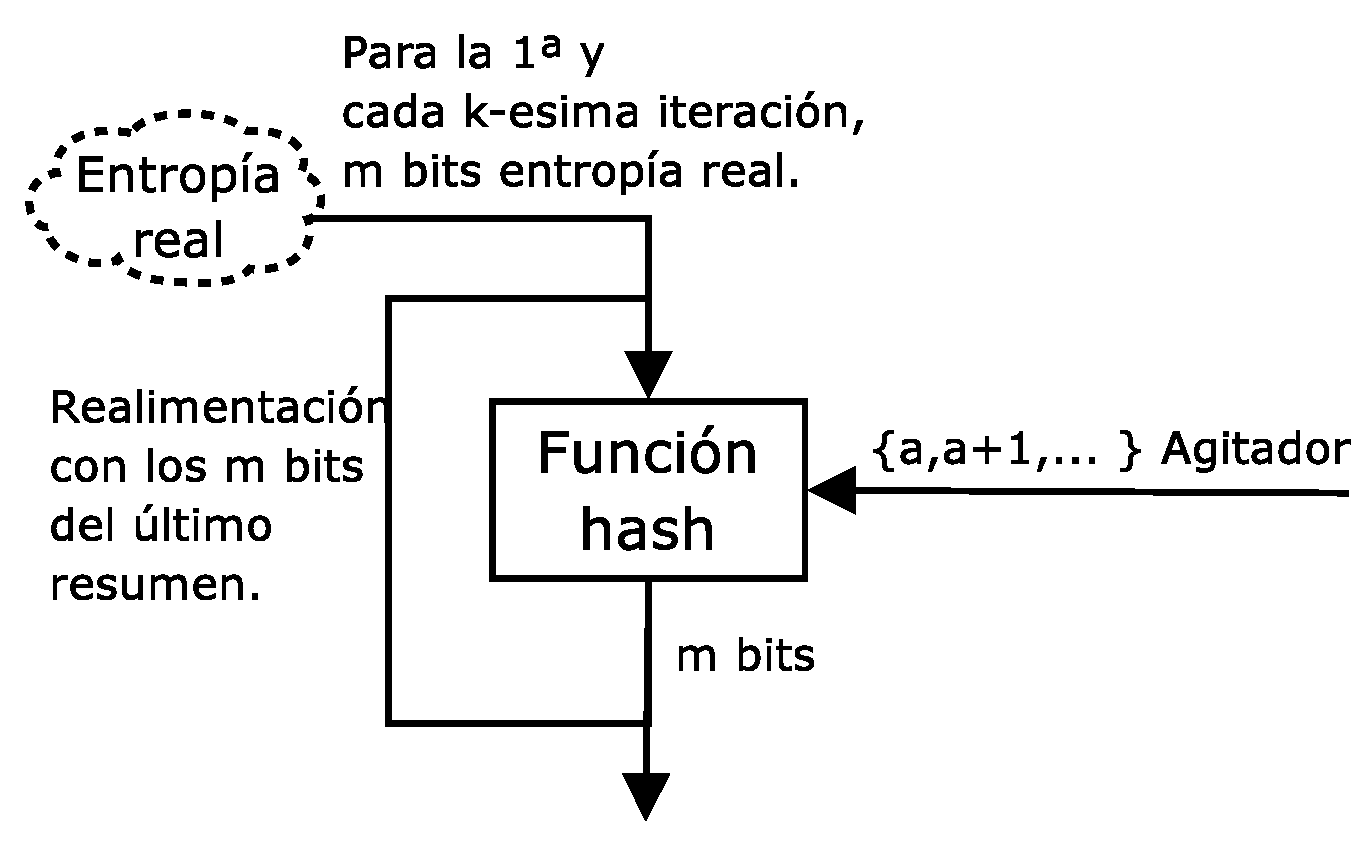
\includegraphics[width=0.8\textwidth,keepaspectratio]{esquemaHashRandom.eps}
     \caption{Esquema con funci�n hash.\label{fig:esquemaHashRandom}}
     \end{center}
    \end{figure}

    \begin{algorithm} 
      \caption{Ciclo semillero} \label{ALGsemillero}
      \begin{algorithmic}[1] 
        \Procedure{leerSemilla}{longitud $L$}
        \State $i \gets 0$
        \State $l \gets 0$
        \State $agitador \gets a$
          \Comment{$a$ puede tomar cualquier valor. Por ejemplo la
          fecha del sistema. No es necesario que sea aleatorio.}
        \State $Q_0 \gets leerDeFuente(m)$
          \Comment{Se leen tantos bits como longitud del resumen que
          la f. hash genera ($m$)}
        \For{$l = 1$ hasta $l = L$}
          \If{$l \geq k$}
            \State $Q_l \gets leerDeFuente(m)$
          \Else
            \State $H(agitador)$ \Comment{$H$ la funci�n hash}
            \State $Q_l \gets H(Q_{l-1})$ 
            \State $agitador \gets agitador+1$
          \EndIf
        \EndFor
        \EndProcedure
      \end{algorithmic}
    \end{algorithm}
        
    
    La idea, una variaci�n de lo propuesto en
    \cite{schneier}\footnote{p�g. 427}, es valerse de la propiedad
    \ref{eq:def2Hash} de las funciones hash (\ref{funcionesHash}) de
    resistencia a preimagen para ``reciclar'' en cada iteraci�n una
    cantidad inicial de entrop�a real de tal forma que invertir el
    proceso sea inviable computacionalmente (un problema
    \emph{dif�cil}) y no se pueda predecir de la $i$-�sima iteraci�n
    y anteriores el valor de los bits obtenidos en la $(i+1)$-�sima.
    Para contribuir a la irreversibilidad de este proceso se pasa
    tambi�n como entrada a la funci�n hash en cada iteraci�n un dato
    ``agitador'' que no ha de ser aleatorio; es m�s, no es
    estrictamente necesario y es posible que no aporte seguridad, pero
    tampoco la quita; s�lo hace que quien pudiera intentar invertir la
    funci�n hash se encuentre no s�lo con un dato de entrada, sino con
    dos. La versi�n en pseudoc�digo y simplificada ---se considera que
    la longitud de la semilla es un m�ltiplo de la longitud del
    resumen de la funci�n hash $m$, cuando en la librer�a se trabaja
    con una precisi�n de bytes--- se muestra en el algoritmo
    \ref{ALGsemillero}.
    
    Est� claro que a medida que este proceso evoluciona, la
    entrop�a real de los datos servidos se va degenerando, por lo que
    cada $k$ iteraciones la entrada a la funci�n hash no ser� el valor
    anterior obtenido de la misma, sino entrop�a real como si de la
    primera iteraci�n se tratase. El valor de este par�metro $k$ ha de
    conjugar el no abusar de la entrop�a del sistema (como suceder�a
    si fuese demasiado peque�o) y el permitir que la entrop�a se degrade en exceso.
    Teniendo en cuenta que cada iteraci�n generar� una cantidad de
    bits que normalmente ser� de $128$ � $160$ (MD5 y SHA-1
    respectivamente), y que en principio a los generadores
    pseudoaleatorios s�lo se les suministrar� una semilla una vez,
    restar� por determinar cu�l es el ``tama�o t�pico'' de una semilla. 
    Pero de nuevo, no existe un valor fijo o de referencia para esto:
    el tama�o que se quiera utilizar depender� de nuestro grado de
    paranoia y/o del valor de los datos a custodiar. \cite{schneier}
    dedica todo un cap�tulo, el s�ptimo, a discutir el �ntimamente
    relacionado tema de la longitud de las claves con el de la
    longitud de la semilla que nos ocupa; a �l se remite al
    lector interesado. De ese cap�tulo aqu� nos quedaremos con lo
    expuesto en su tabla 7.10, donde se manejan longitudes en bits de
    $64$ a $128$ para seguridad contra ataques por fuerza bruta que
    oscilan en su duraci�n de horas a siglos. Teniendo en cuenta que
    dicha tabla probablemente tenga ya cerca de diez a�os de
    antig�edad, y que el ser pesimista en este sentido es positivo,
    doblemos esas cantidades; $256$ bits ser� un tama�o de semilla
    suficientemente grande para que un atacante que tuviera que buscar
    por un espacio de $2^{256}$ se lo pensase dos veces ---el espacio en
    el que buscar es precisamente igual a todas las combinaciones ya
    que estamos suponiendo que a ojos del atacante todas las
    combinaciones son equiprobables, como idealmente habr�an de ser.
    As� que, concluyendo, se gastar�n dos iteraciones en cada nueva
    semilla generada. Un valor de $10$ iteraciones antes de regenerar
    el esquema con entrop�a real parece adecuado; dar�a para
    inicializar ocho generadores distintos, algo extremadamente raro
    en un programa, donde se utilizar� normalmente s�lo uno. Y si el
    caso es que se utilizan semillas de un tama�o mayor de $256$ bits,
    est� justificado regenerar con esa frecuencia, ya que tal semilla
    s�lo ser�a necesaria en aplicaciones de alt�sima seguridad,
    justificando pues el gasto de entrop�a real.
    

    Pero a�n no se ha tratado el problema de la obtenci�n de la
    entrop�a real. Pues bien, este problema, debido a todo lo apuntado
    con anterioridad, se delega al sistema operativo. Y esto se hace
    as� ya que es el �nico que est� en situaci�n de acceder a los
    dispositivos de bajo nivel pertinentes para recolectar entrop�a.
    Examinar la frecuencia de pulsaciones en el teclado o analizar el
    movimiento del rat�n es algo que se escapa por completo a la
    capacidad de un programa que resida fuera del n�cleo del sistema.
    Hacerlo pasar�a por tener que realizar llamadas al sistema de muy
    bajo nivel con todo lo que ello implica: romper la portabilidad,
    necesidad de asignar unos permisos especiales que representar�an
    una potencial brecha de seguridad, etc. Y eso sin tener en cuenta
    toda la compleja manipulaci�n de la entrop�a y tratamiento de los
    citados sesgos en los datos recolectados. �No se est� entonces
    violando uno de los objetivos de la librer�a, su portabilidad? S�
    y no. Por una parte est� claro que si uno ha de valerse del
    sistema operativo para algo, se vuelve dependiente de �ste. Pero
    al ser las necesidades de entrop�a algo relativamente com�n y por
    lo expuesto antes, s�lo susceptible de ser realizado por el
    sistema operativo, estos mecanismos est�n presentes en la pr�ctica
    totalidad de los sistemas, y en muchos de ellos de forma id�ntica:
    la gran mayor�a de los sistemas derivados o basados en UNIX
    ofrecen un dispositivo especial \texttt{/dev/random} y/o
    \texttt{/dev/urandom} que tratado como un fichero ordinario
    permite obtener esta entrop�a recolectada por el sistema. El
    c�digo que implementa esta funcionalidad en la versi�n 2.6.5 de
    Linux se puede leer:
    \begin{quotation}
      Computers are very predictable devices.  Hence it is extremely hard
      to produce truly random numbers on a computer. [\ldots] we must try to
      gather ``environmental noise'' from the computer's environment, which
      must be hard for outside attackers to observe, and use that to
      generate random numbers.  In a Unix environment, this is best done
      from inside the kernel.
      
      Sources of randomness from the environment include \emph{inter-keyboard
      timings}, \emph{inter-interrupt timings from some interrupts}, and other
      events which are both (a) non-deterministic and (b) hard for an
      outside observer to measure. \footnote{Sin los �nfasis en el original.}
    \end{quotation}
    Se comenta en ese mismo archivo ( \texttt{drivers/char/random.c}
    dentro de la jerarqu�a de las fuentes del n�cleo ) las t�cnicas
    utilizadas para el tratamiento de los datos y dem�s aspectos muy
    interesantes.

    Para el otro gran conjunto de sistemas, los sistemas basados en
    Microsoft Windows, esta funcionalidad no est� tan a la vista,
    siendo proporcionada por el ``Crypto API'' mediante la funci�n
    \texttt{CryptGenRandom}, documentada en \\
    \texttt{http://msdn.microsoft.com/library/en-us/security/security/cryptgenrandom.asp}.
    All� se lee lo siguiente:
    \begin{quotation}
      CryptoAPI stores an intermediate random seed with every
      user. To form the seed for the random number generator, a calling application
      supplies bits it might have for instance, \emph{mouse or keyboard timing input} that
      are then added to both the stored seed and various system data and user data
      such as the \emph{process ID} and \emph{thread ID}, \emph{the system clock}, 
      \emph{the system time}, \emph{the 
      system counter}, \emph{memory status}, \emph{free disk clusters},
      \emph{the hashed user environment block}. 
      \footnote{Sin los �nfasis en el original.}
    \end{quotation}
    Como era de esperar, ambos sistemas utilizan b�sicamente unas
    fuentes de entrop�a similares.

    As� pues, conceder un peque�o permiso a la utilizaci�n de estas
    funciones dependientes del sistema aporta numerosas ventajas con
    un impacto m�nimo a la portabilidad: a�n en el caso de no estar en
    un sistema que no ofreciese ninguno de los mecanismos citados,
    todo cambio pasar�a tan s�lo por implementar un �nico m�todo de la
    clase que implementa el semillero de la manera que consideremos
    oportuna. El autor confiesa no conocer ning�n sistema operativo
    que no brinde uno de los dos m�todos citados.
    



% CAPITULO SOBRE FUNCIONES TRASCENDENTES

\chapter{Funciones trascendentes}\label{cap:primos}

\begin{flushright}
  \begin{minipage}[t]{13cm}
    \begin{flushright}
      \begin{quote}
        \emph{
         cita
        }
        \begin{flushright}
          \textbf{\textemdash D. Zagier}
        \end{flushright}
      \end{quote}
    \end{flushright}
  \end{minipage}
\end{flushright}

\bigskip

\begin{flushright}
  \begin{minipage}[t]{13cm}
    \begin{flushright}
      \begin{quote}
        \emph{
        cita 2
        }
        \begin{flushright}
          \textbf{\textemdash H. Montgomery}
        \end{flushright}
      \end{quote}
    \end{flushright}
  \end{minipage}
\end{flushright}

\bigskip

\begin{center}{\line(1,0){325}}\end{center}

%--------------------------------------------------------%

\section{Introducci�n}
\section{La funci�n exponencial}
  
  \subsection{Exponencial inversa: la funci�n logaritmo}
    \begin{observacion}\label{obsLog}
      Si $x \in \mathbb{R}$, existe un $n \in \mathbb{N}$ tal que
      $2^{n-1} < x \leq 2^n$. Entonces, si $y = x/2^n$, se verifica
      que $0 < y \leq 1$
    \end{observacion}

    En base a la observaci�n \ref{obsLog}, el c�lculo de $x \in
    \mathbb{R}$ se reducir�a a (utilizando los s�mbolos de dicha
    observaci�n):
    \[
      \log{(x)} = \log{(y \times 2^n)} = \log{(y)} + n \cdot \log{(2)}
    \]
    Las ventajas que de esta forma de calcula el logaritmo se
    desprenden son claras: por una parte, el c�lculo de $\log(2)$ (tambi�n denominada
    ``La constante logar�tmica'', v�ase \cite{log2}) es un problema
    ampliamente tratado y existen m�todos de gran eficiencia para su c�lculo. 
    M�s adelante se tratar� este punto en m�s profundidad.
    Por otra parte, al cumplirse $0 < y \leq 1$, el c�lculo de
    $\log{(y)}$ puede realizarse satisfactoriamente y con relativa
    efectividad utilizando la expansi�n de MacLaurin
    para la funci�n logaritmo.

    \subsubsection{La constante logar�tmica}

    


  
\section{Funciones trigonom�tricas}

  \subsection{El c�lculo de las inversas}



%% CAPITULO SOBRE LAS DEMOSTRACIONES Y COMPARACI�N

\chapter{Ejemplos y comparativa}

\begin{flushright}
  \begin{minipage}[t]{13cm}
    \begin{flushright}
      \begin{quote}
        \emph{
        Las palabras son enanos, los ejemplos son gigantes.
        }
        \begin{flushright}
          \textbf{\textemdash Proverbio suizo.}
        \end{flushright}
      \end{quote}
    \end{flushright}
  \end{minipage}
\end{flushright}

\begin{center}{\line(1,0){325}}\end{center}

%--------------------------------------------------------%

 
  

%% CAPITULO SOBRE LAS POSIBLES MEJORAS, AMPLIACIONES Y CRITICA

\chapter{Cr�tica}

\begin{flushright}
  \begin{minipage}[t]{13cm}
    \begin{flushright}
      \begin{quote}
        \emph{
          Become addicted to constant and never-ending self improvement.
        }
        \begin{flushright}
          \textbf{\textemdash Anthony J. D'Angelo, The College Blue Book}
        \end{flushright}
      \end{quote}
    \end{flushright}
  \end{minipage}
\end{flushright}

\begin{center}{\line(1,0){325}}\end{center}

%--------------------------------------------------------%

\section{Posibles mejoras}
  \subsection{Mayor aprovechamiento de instrucciones SIMD}
    En las operaciones con matrices.

\section{Ampliaciones}
  \subsection{Sobre Polinomios}
    \subsubsection{Factorizaci�n}
      Al igual que para la factorizaci�n de enteros, no se conoce
      un m�todo que permita realizar esta operaci�n en un tiempo razonable. Como es habitual
      en este contexto, �razonable� suele traducirse como �computable en tiempo polinomial�.
      %TODO
  \subsection{Sobre cuerpos finitos}
    En la implementaci�n actual los cuerpos finitos $\GF{p^n}$, 
    se modela $p$ como un entero de tipo \texttt{mpplas::Z}; es decir,
    un entero de precisi�n arbitraria. En la mayor�a de los casos, la caracter�stica de la precisi�n arbitraria
    no es explotada, y de hecho influye negativamente en el rendimiento. De hecho, es usual el uso de cuerpos
    finitos de la forma $\GF{2^n}$. En este caso, es posible explotar el car�cter binario de los elementos.
    Por ejemplo, la suma se reduce a una operaci�n o-exclusivo a nivel de bits. 

    En cualquier caso, la presente biblioteca se centra entorno a tipos de precisi�n arbitraria, raz�n por la cual
    esta caracter�stica tendr�a m�s cabida en otro tipo de biblioteca.


\section{Conclusiones}
  


% PRUEBAS BORRADOR

\chapter{Pruebas, \textbf{BORRADOR}}
\section{Casos de prueba por funci�n}
\begin{itemize}
  \item divMP(vector, vector)
    \begin{itemize}
      \item[-] Ejemplo: Un entero igual a
        $79228162514264337593543950336 = 2^{32+64}$ y otro igual a 
        $4294967296 = 2^{32}$. Su divisi�n provoca a fecha 21 de Enero 
        que falle la divisi�n debido a que el tama�o del dividendo 
        disminuye m�s r�pido que de uno en uno, mientras que la guarda
        del bucle ``principal'' disminuye de uno en uno.\\
        \textbf{Soluci�n}: La guarda del bucle debe actualizarse en
        funci�n de la variaci�n de tama�o del dividendo.
    \end{itemize}
\end{itemize}

        
        

%%%%%%%%%%%%%%%%%%%%%%%%%%%%%%%%%%%%%%%%%%%%%%%%%%%%%

\bibliographystyle{proyecto}
\bibliography{biblbibliografia}

\printindex

\end{document}
